%-------------------------------------------------------------------------------
% This file provides a skeleton ATLAS note.
%-------------------------------------------------------------------------------
% Specify where ATLAS LaTeX style files can be found.
\newcommand*{\ATLASLATEXPATH}{latex/}
% Use this variant if the files are in a central location, e.g. $HOME/texmf.
% \newcommand*{\ATLASLATEXPATH}{}
%-------------------------------------------------------------------------------
%\documentclass[NOTE, USenglish, texlive=2017]{\ATLASLATEXPATH atlasdoc}
\documentclass[NOTE, english, texlive=2017]{\ATLASLATEXPATH atlasdoc}
%\documentclass[NOTE, USenglish, texlive=2017]{\ATLASLATEXPATH atlasdoc}
% The language of the document must be set: usually UKenglish or USenglish.
% british and american also work!
% Commonly used options:
%  texlive=YYYY          Specify TeX Live version (2016 is default).
%  coverpage             Create ATLAS draft cover page for collaboration circulation.
%                        See atlas-draft-cover.tex for a list of variables that should be defined.
%  cernpreprint          Create front page for a CERN preprint.
%                        See atlas-preprint-cover.tex for a list of variables that should be defined.
%  NOTE                  The document is an ATLAS note (draft).
%  PAPER                 The document is an ATLAS paper (draft).
%  CONF                  The document is a CONF note (draft).
%  PUB                   The document is a PUB note (draft).
%  BOOK                  The document is of book form, like an LOI or TDR (draft)
%  txfonts=true|false    Use txfonts rather than the default newtx
%  paper=a4|letter       Set paper size to A4 (default) or letter.

%-------------------------------------------------------------------------------
% Extra packages:
\usepackage{\ATLASLATEXPATH atlaspackage}
% Commonly used options:
%  biblatex=true|false   Use biblatex (default) or bibtex for the bibliography.
%  backend=bibtex        Use the bibtex backend rather than biber.
%  subfigure|subfig|subcaption  to use one of these packages for figures in figures.
%  minimal               Minimal set of packages.
%  default               Standard set of packages.
%  full                  Full set of packages.
%-------------------------------------------------------------------------------
% Style file with biblatex options for ATLAS documents.
\usepackage{\ATLASLATEXPATH atlasbiblatex}

% Package for creating list of authors and contributors to the analysis.
\usepackage{\ATLASLATEXPATH atlascontribute}

% Useful macros
\usepackage{\ATLASLATEXPATH atlasphysics}
% See doc/atlas_physics.pdf for a list of the defined symbols.
% Default options are:
%   true:  journal, misc, particle, unit, xref
%   false: BSM, heppparticle, hepprocess, hion, jetetmiss, math, process, other, texmf
% See the package for details on the options.

% Files with references for use with biblatex.
% Note that biber gives an error if it finds empty bib files.
\addbibresource{DispDilep-INT-2017.bib}
\addbibresource{bib/ATLAS.bib}
\addbibresource{bib/CMS.bib}
\addbibresource{bib/ConfNotes.bib}
\addbibresource{bib/PubNotes.bib}

% Paths for figures - do not forget the / at the end of the directory name.
\graphicspath{{logos/}{figures/}}

% Add you own definitions here (file DispDilep-INT-2017-defs.sty).
\usepackage{DispDilep-INT-2017-defs}
\usepackage{multirow}
%\usepackage{floatrow}
\usepackage[utf8]{inputenc}
\captionsetup[subfloat]{captionskip=1pt}
%\setlength\abovecaptionskip{-5pt}
%-------------------------------------------------------------------------------
% Generic document information
%-------------------------------------------------------------------------------

% Title, abstract and document 
%-------------------------------------------------------------------------------
% This file contains the title, author and abstract.
% It also contains all relevant document numbers used for an ATLAS note.
%-------------------------------------------------------------------------------

% Title
%\AtlasTitle{Search for long-lived neutral massive particle with displaced dilepton resonance at the LHC}
\AtlasTitle{Search for long-lived resonance decaying to a dilepton pair in $pp$ collisions at $\sqrt{s}=13$ TeV with the ATLAS detector}

% Draft version:
% Should be 1.0 for the first circulation, and 2.0 for the second circulation.
% If given, adds draft version on front page, a 'DRAFT' box on top of each other page, 
% and line numbers.
% Comment or remove in final version.
\AtlasVersion{0.1}

% Abstract - % directly after { is important for correct indentation
\AtlasAbstract{%
A search for long-lived neutral massive particle decaying to a $\mu\mu$, $ee$, or $e\mu$ pair is presented using the ATLAS detector with 32.8 $\mathrm{fb^{-1}}$ of $pp$ collisions at $\sqrt{s}=13$ TeV at the LHC. %No significant deviation from the Standard Model is observed.
Upper limits are presented on the production cross section times branching ratio for resonances decaying to a lepton pair. Also presented is the detection efficiency as a function of $p_{T}$ and $\eta$ for a resonance with mass of 0.1$-$2.0 TeV and lifetime ($c\tau$) of 100$-$500 mm.
}

% Author - this does not work with revtex (add it after \begin{document})
% \author{The ATLAS Collaboration}

% Authors and list of contributors to the analysis
% \AtlasAuthorContributor also adds the name to the author list
% Include package latex/atlascontribute to use this
% Use authblk package if there are multiple authors, which is included by latex/atlascontribute
% \usepackage{authblk}
% Use the following 3 lines to have all institutes on one line
% \makeatletter
% \renewcommand\AB@affilsepx{, \protect\Affilfont}
% \makeatother
% \renewcommand\Authands{, } % avoid ``. and'' for last author
% \renewcommand\Affilfont{\itshape\small} % affiliation formatting
\AtlasAuthorContributor{Siinn Che}{a}{Main analyzer}
\AtlasAuthorContributor{K.K. Gan}{a}{Advisor}
\AtlasAuthorContributor{Christopher B. Martin}{a}{Main analyzer}
% \AtlasAuthorContributor{Christopher B. Martin}{a}{Main analyzer}
% \AtlasAuthorContributor{Third AtlasAuthorContributor}{a}{Author's contribution.}
% \AtlasContributor{Fourth AtlasContributor}{Contribution to the analysis.}
% \author[a]{First Author}
% \author[a]{Second Author}
% \author[b]{Third Author}
\affil[a]{The Ohio State University}
% \affil[b]{Another Institution}

% If a special author list should be indicated via a link use the following code:
% Include the two lines below if you do not use atlasstyle:
% \usepackage[marginal,hang]{footmisc}
% \setlength{\footnotemargin}{0.5em}
% Use the following lines in all cases:
%\usepackage{authblk}
%\author{The ATLAS Collaboration%
%\thanks{The full author list can be found at:\newline
%  \url{https://atlas.web.cern.ch/Atlas/PUBNOTES/ATL-PHYS-PUB-2016-007/authorlist.pdf}}
% }

% ATLAS reference code, to help ATLAS members to locate the paper
\AtlasRefCode{EXOT-2017-XX}

% ATLAS note number. Can be an COM, INT, PUB or CONF note
% \AtlasNote{ATLAS-CONF-2016-XXX}
% \AtlasNote{ATL-PHYS-PUB-2016-XXX}
% \AtlasNote{ATL-COM-PHYS-2016-XXX}

% Author and title for the PDF file
\hypersetup{pdftitle={ATLAS document},pdfauthor={The ATLAS Collaboration}}


%-------------------------------------------------------------------------------
% Content
%-------------------------------------------------------------------------------
\begin{document}

\maketitle

\tableofcontents

% List of contributors - print here or after the Bibliography.
%\PrintAtlasContribute{0.30}
%\clearpage

%-------------------------------------------------------------------------------
\section{Introduction}
\label{sec:intro}
%This displaced vertex signature has the potential to provide an evidence for Physics beyond the SM, and it provides very clean signature with minimum backgrounds from the SM processes.
The search for long-lived particles (LLP) is an important part of the program in searching for new physics at the LHC. Many extensions to the Standard Model (SM) such as split SUSY~\cite{Hewett:2004nw}~\cite{ArkaniHamed:2004yi}, MSSM with R-parity violation~\cite{Barbier:2004ez}, or Hidden Valley~\cite{Han:2007ae} predict the production of neutral, weakly-coupled particles with long lifetimes compatible with the dimension of the ATLAS detector. In particular, several theories, including R-parity violation, Hidden valley, or $Z'$ models with long-lived neutrinos~\cite{Basso:2008iv}, predict the existence of LLPs that can decay to final-states containing a displaced vertex with a pair of leptons.

This paper presents the search for a heavy, long-lived neutral particle decaying to a dilepton pair, $\mu\mu$, $ee$, or $e\mu$ within the ATLAS Inner Detector (ID). The LLP is referred as $Z'$ but with no assumption on $Z'$ production mechanism for a model-independent search. For the purpose of establishing a signal benchmark, the LLP is singly produced in Drell-Yan process with $Z'$ mass ranges from 100 GeV to 1 TeV and $c\tau$ between 100 mm and 500 mm. The displaced vertex provides a clean signature with minimum backgrounds from the SM processes.

There have been several searches for the LLPs produced in $pp$ collisions in Run I at $\sqrt{s} =$ 8 TeV, including the search for displaced hadronic jet~\cite{Blackburn:1550730}, displaced heavy flavors~\cite{Harris:1512932}, or multi-track displaced vertex~\cite{Aad:2015rba}, and no significant excess was observed. This paper presents the search for a different signature, and it is one of the first efforts\footnote{SUSY displaced dilepton search in Run II is looking for a displaced dilepton signature in the context of supersymmetric models.} in the ATLAS experiment to search for a genetic displaced vertex signature decaying to a dilepton pair.

This analysis uses 32.8 $\mathrm{fb^{-1}}$ of $pp$ collision data at $\sqrt{s}=13$ TeV collected in 2016 using the ATLAS detector. In order to gain sensitivity for the non-conventional signature of LLPs, a special setup of data reprocessing and reconstruction, called \textit{Large radius tracking}, is used. This setup is described in ~\ref{sec:track_vertex_reconstruction}. The special setup allows the reconstruction of tracks with large impact parameters and secondary vertices significantly displaced from primary vertices.

The analysis shares the technical setup and the analysis framework~\cite{SUSYAnalysisFramework} with SUSY displaced multi-track vertex search~\cite{Duarte-Campderros:2152010} and SUSY displaced dilepton search~\cite{}. The former searches for the LLPs decaying to displaced vertices with high track multiplicity and large missing energy, and the latter looks for the same displaced dilepton signature as this search but in the context of supersymmetric models. 

%This analysis focuses on interpreting the displaced dilepton from a LLP decay in the context of model-independent, Exotics search.
This analysis focuses on interpreting the LLPs decaying to displaced dilepton vertices in the context of model-independent, exotic resonance search.



%-------------------------------------------------------------------------------
\section{Data and MC samples}
\label{sec:data_MC}
\subsection{Data samples}
\label{sec:data_sample}

The analysis uses the full 2016 $pp$ collisions data (periods A-L) with the integrated luminosity of 32.8 $\mathrm{fb^{-1}}$. In this search, because the standard ATLAS track reconstruction does not provide good sensitivity for long-lived particles, a dedicated stream, \texttt{DRAW\_RPVLL}, is used to reconstruct events using the non-standard reconstruction algorithm discussed in Section~\ref{sec:large_radius_tracking}. The stream is used in several Exotics and SUSY analyses, searching for long-lived particles. %non-standard reconstruction objects.

In \texttt{DRAW\_RPVLL} stream, a subset of events from the main physics stream is selected by \texttt{RPVLL} filters. The filters select events using High-Level Triggers (HLT) and offline selections configured for each analysis. The triggers and offline selection used in this search is discussed in Section~\ref{sec:signal_selection}. The selected events are passed downstream for reconstruction. The data is in \texttt{RAW} format so that low-level information such as detector hits can be used for the special reconstruction algorithms to reconstruct displaced tracks and vertices.
%The low-level data available in \texttt{RAW} data, such as detector hits, allows the special reconstruction algorithms to reconstruct displaced tracks and displaced vertices.

The selected events are centrally processed with AMI tag \texttt{r8669}. The dedicated track reconstruction algorithm, the \textit{large radius tracking}, and the secondary vertex reconstruction algorithm, \texttt{VrtSecInclusive}, are used to reconstruct displaced tracks and vertices, respectively. The output of \texttt{DRAW\_RPVLL} stream is in \texttt{DAOD\_RPVLL} format which is a standard \texttt{xAOD} data format with additional displaced tracks and secondary vertices reconstructed. 

The \texttt{DAOD\_RPVLL} is further processed to produce the \texttt{DAOD\_SUSY15} derivation with \texttt{AODfix} and data reduction as recommended by the Analysis Model Study Group (AMSG)~\cite{Catmore:1543445}. Table~\ref{table:data_samples} summarizes datasets used in this search.

\begin{table}[!htb]
  \centering
  \begin{tabular}{ l l }
    \hline
    \hline
    Format     				& Dataset       													\\
    \hline
	\texttt{DRAW\_RPVLL}	& data16\_13TeV.*.physics\_Main.merge.DRAW\_RPVLL.f*\_m*			\\
	\texttt{DAOD\_RPVLL}	& data16\_13TeV.*.physics\_Main.recon.DAOD\_RPVLL.f*\_r8669			\\
	\texttt{DAOD\_SUSY15}	& data16\_13TeV.*.physics\_Main.recon.DAOD\_RPVLL.f*\_r8669\_p2950	\\
    \hline
    \hline
  \end{tabular}
  \caption{Dataset used in \texttt{DRAW\_RPVLL}, \texttt{DAOD\_RPVLL}, and \texttt{DAOD\_SUSY15} format.}
  \label{table:data_samples}
\end{table}

This search uses a modified version of the standard \texttt{GoodRunsList} because a small number of events selected by \texttt{DRAW\_RPVLL} was not reconstructed successfully. The corresponding lumi blocks were removed from the \texttt{GoodRunsList}\footnote{\texttt{data16\_13TeV.periodAllYear\_DetStatus-v83-pro20-15\_DQDefects-00-02-04\_PHYS\_StandardGRL\_All\_Good\\\_25ns\_DAOD\_RPVLL\_r8669.xml}}.

\subsection{MC samples}
\label{sec:mc_sample}

\subsubsection{Signal samples}
\label{sec:signal_sample}
The long-lived $Z'$ is generated using \texttt{PYTHIA 6.4}~\cite{1126-6708-2006-05-026} in which $Z'$ is singly produced from $q\bar{q}$ scattering and decays to a $\mu\mu$, $ee$, or $e\mu$ pair. The proper lifetime, $c\tau$, is set to 100 mm, 250 mm, or 500 mm. The mass of $Z'$ is set between 100 and 1000 GeV. A width based on relativistic Breit-Wigner is assumed for the new resonance. A sample of 20k events are generated for each mass and lifetime. Table~\ref{table:MC_signal_samples} summarizes dataset identifiers (DIDs), mass, and lifetime of the signal MC samples used in this search.

\begin{table}[!htb]
  \centering
  \begin{tabular}{ c c c c c c c }
    \hline
    \hline
           &   &    & \multicolumn{3}{c}{DID}                 \\
    $m_{Z'}$ (GeV) & $\Gamma$ (GeV) & $c\tau$ (mm) &$\mu\mu$ & $ee$ & $e\mu$ \\
    \hline
    100			   &	2.8         &   100	& 308264	& 309539		&	309554		\\
    100			   &	2.8         &   250	& 308265	& 309540		&	309555		\\
    100			   &	2.8         &   500	& 308266	& 309541		&	309556		\\
    250			   &   6.9	        &   100	& 301911	& 309542		&	309557		\\
    250			   &	6.9         &   250	& 301912	& 309543		&	309558		\\
    250			   &	6.9         &   500	& 301913	& 309544		&	309559		\\
    500			   &   14.7         &   100	& 301914	& 309545		&	309560		\\
    500			   &	14.7        &   250	& 301915	& 309546		&	309561		\\
    500			   &	14.7        &   500	& 301916	& 309547		&	309562		\\
    750			   &	23.0        &   100	& 308285	& 309548		&	309563		\\
    750			   &	23.0        &   250	& 308286	& 309549		&	309564		\\
    750			   &	23.0        &   500	& 308287	& 309550		&	309565		\\
    1000	       &	31.0        &   100	& 301917	& 309551		&	309566		\\
    1000	       &	31.0        &   250	& 301918	& 309552		&	309567		\\
    1000	       &	31.0        &   500	& 301919	& 309553		&	309568		\\
    \hline
    \hline
  \end{tabular}
  \caption{Mass, lifetime, and DID of the signal MC samples.}
  \label{table:MC_signal_samples}
\end{table}
%\begin{table}[!htb]
%  \centering
%  \begin{tabular}{ c c c c c c c }
%    \hline
%    \hline
%           &   &    & \multicolumn{3}{c}{DID}                 \\
%    $m_{Z'}$ (GeV) & $\Gamma$ (GeV) & $c\tau$ (mm) & $\sigma$ (pb) &$\mu\mu$ & $ee$ & $e\mu$ \\
%    \hline
%    100			   &	2.8         &   100	& 1104 & 308264	& -		&	-		\\
%    100			   &	2.8         &   250	& 1104 & 308265	& -		&	-		\\
%    100			   &	2.8         &   500	& 1104 & 308266	& -		&	-		\\
%    250			   &   6.9	        &   100	& 64.60 & 301911	& -		&	-		\\
%    250			   &	6.9         &   250	& 64.04 & 301912	& -		&	-		\\
%    250			   &	6.9         &   500	& 64.14 & 301913	& -		&	-		\\
%    500			   &   14.7         &   100	& 5.773 & 301914	& -		&	-		\\
%    500			   &	14.7        &   250	& 5.769 & 301915	& -		&	-		\\
%    500			   &	14.7        &   500	& 5.747 & 301916	& -		&	-		\\
%    750			   &	23.0        &   100	& 1.236 & 308285	& -		&	-		\\
%    750			   &	23.0        &   250	& 1.236 & 308286	& -		&	-		\\
%    750			   &	23.0        &   500	& 1.236 & 308287	& -		&	-		\\
%    1000	       &	31.0        &   100	& 0.3902 & 301917	& -		&	-		\\
%    1000	       &	31.0        &   250	& 0.3902 & 301918	& -		&	-		\\
%    1000	       &	31.0        &   500	& 0.3848 & 301919	& -		&	-		\\
%    \hline
%    \hline
%  \end{tabular}
%  \caption{Mass, lifetime, and DID of the signal MC samples.}
%  \label{table:MC_signal_samples}
%\end{table}

The signal MC samples generated by \texttt{PYTHIA} are processed to include detector simulation using the AMI tags \texttt{s2698} and \texttt{s2726}. The samples are overlaid with simulated minimum-bias events to model multiple interactions (pile-up) in data samples. In the signal MC samples, the average number of pile-ups, $\langle\mu\rangle$, ranges from 10 to 40 with small number of events having $\langle\mu\rangle$ < 10. The difference in the $\langle\mu\rangle$ distributions between MC and data samples are corrected for by pile-up reweighting in Section~\ref{sec:efficiency_reweighting}. The resulting MC samples, in \texttt{HITS} format, are reconstructed using AMI tag \texttt{r8788}.

In the reconstruction process, the large radius tracking and \texttt{VrtSecInclusive} algorithms are used with the same configuration as data samples discussed in Section~\ref{sec:data_sample}, to reconstruct displaced tracks and vertices. The reconstructed events are stored in \texttt{DAOD\_RPVLL}, and the samples are processed to produce the \texttt{DAOD\_SUSY15} derivation with \texttt{AODfix} and data reduction. 

The representative plots of truth-level $p_{T}$ and $\eta$ distributions of $Z'$ and the muons from the decay of $Z'$, referred as \textit{signal} muons, are shown in Figure~\ref{fig:truth_zp_muon} using the signal MC samples with $m=$ 500, 1000 GeV and $c\tau=$ 100 mm. The signal MC samples with $ee$ and $e\mu$ final states produce similar distributions as shown in Appendix~\ref{app:signal_truth}.

%The $\eta$ distribution of $Z'$ shows a forward distribution, and it is reweighted to a flat $\eta$ distribution to provide model-independent result. The details are discussed in Section~\ref{sec:efficiency_reweighting}.
The $\eta$ distribution of signal muons shows that most of the signal muons are produced within the detector acceptance ($\eta <$ 2.7). The characteristic upper edge in the $p_{T}$ spectrum is related to the $Z'$ mass.
%The $p_{T}$ distribution of muons shows that muon $p_{T}$ is constrained by the $Z'$ mass.


\begin{figure}[!htb]
    \centering
    \subfloat[]{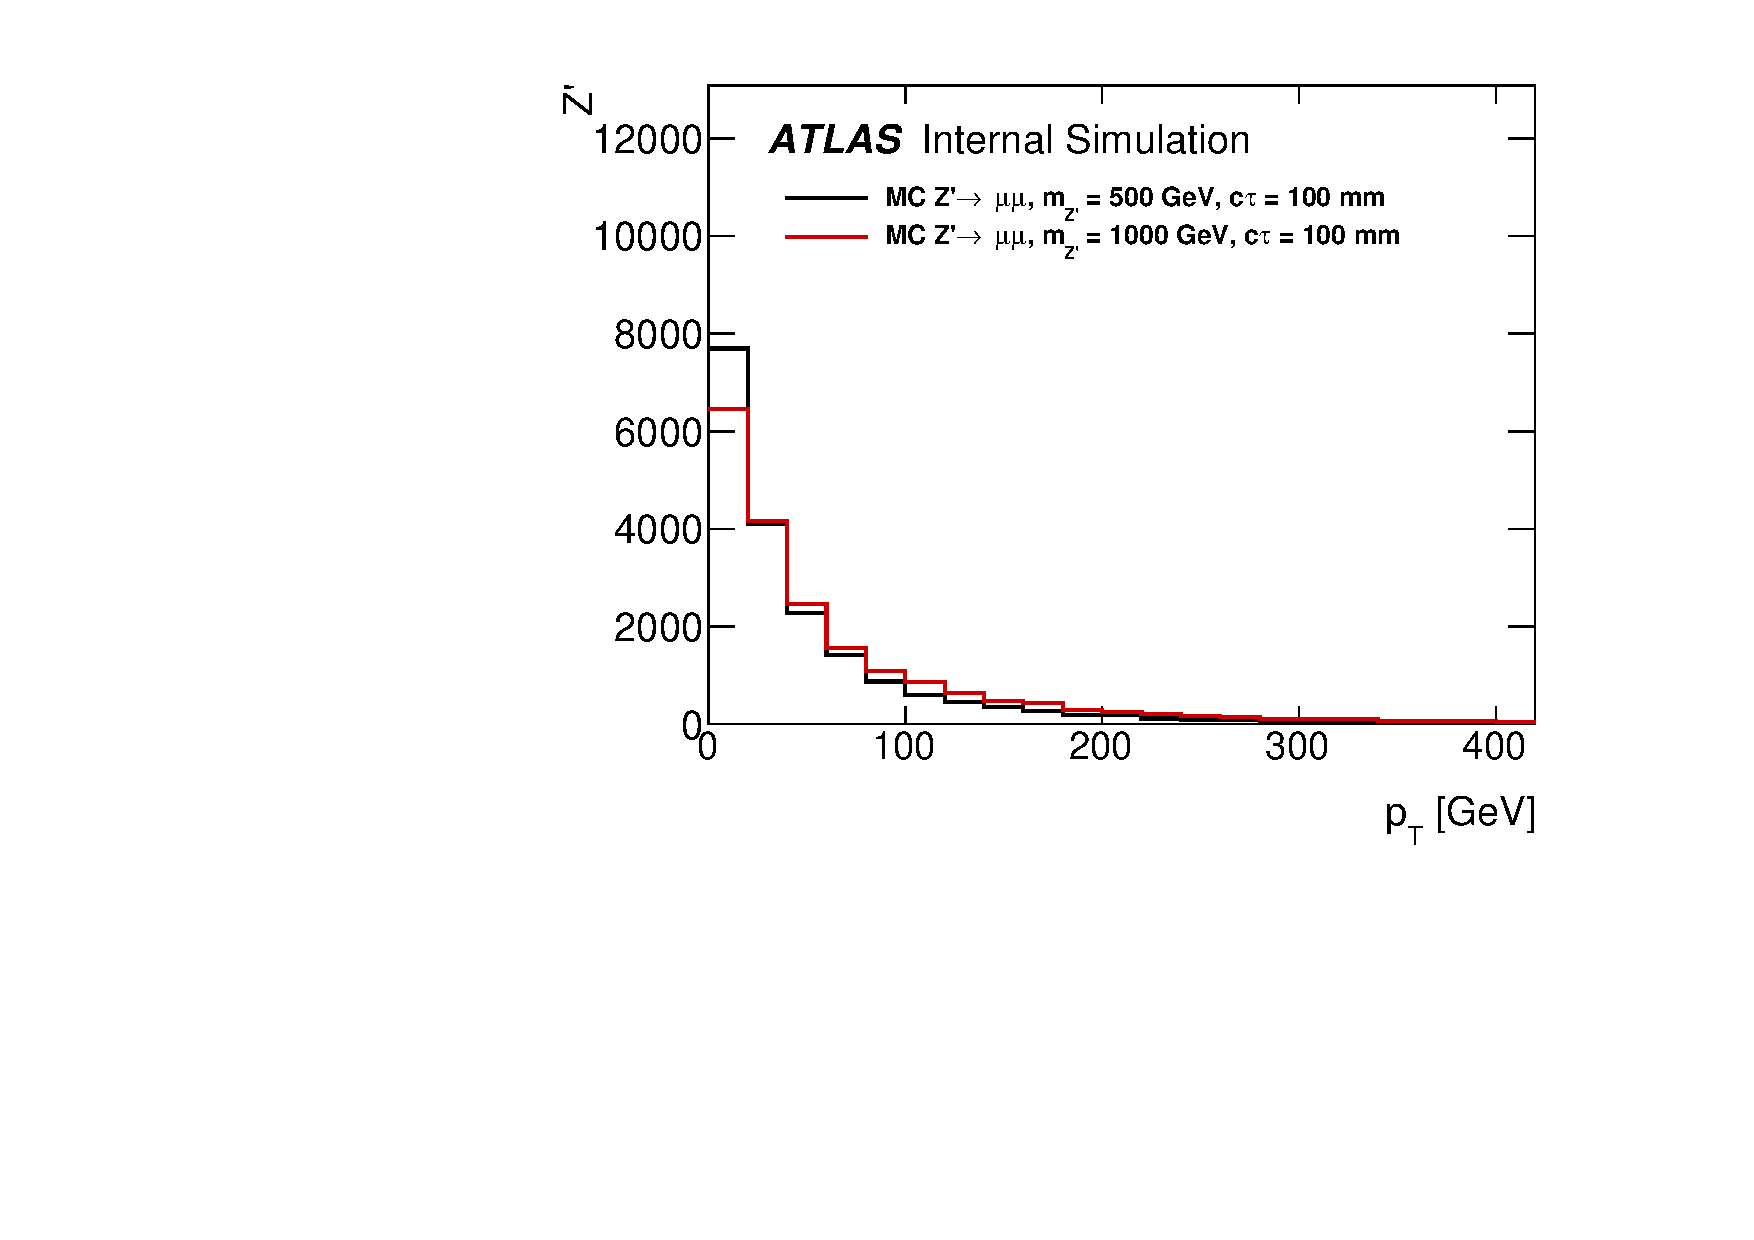
\includegraphics[width=0.45\textwidth]{figures/m_truth_zp_pt.pdf}}
    \subfloat[]{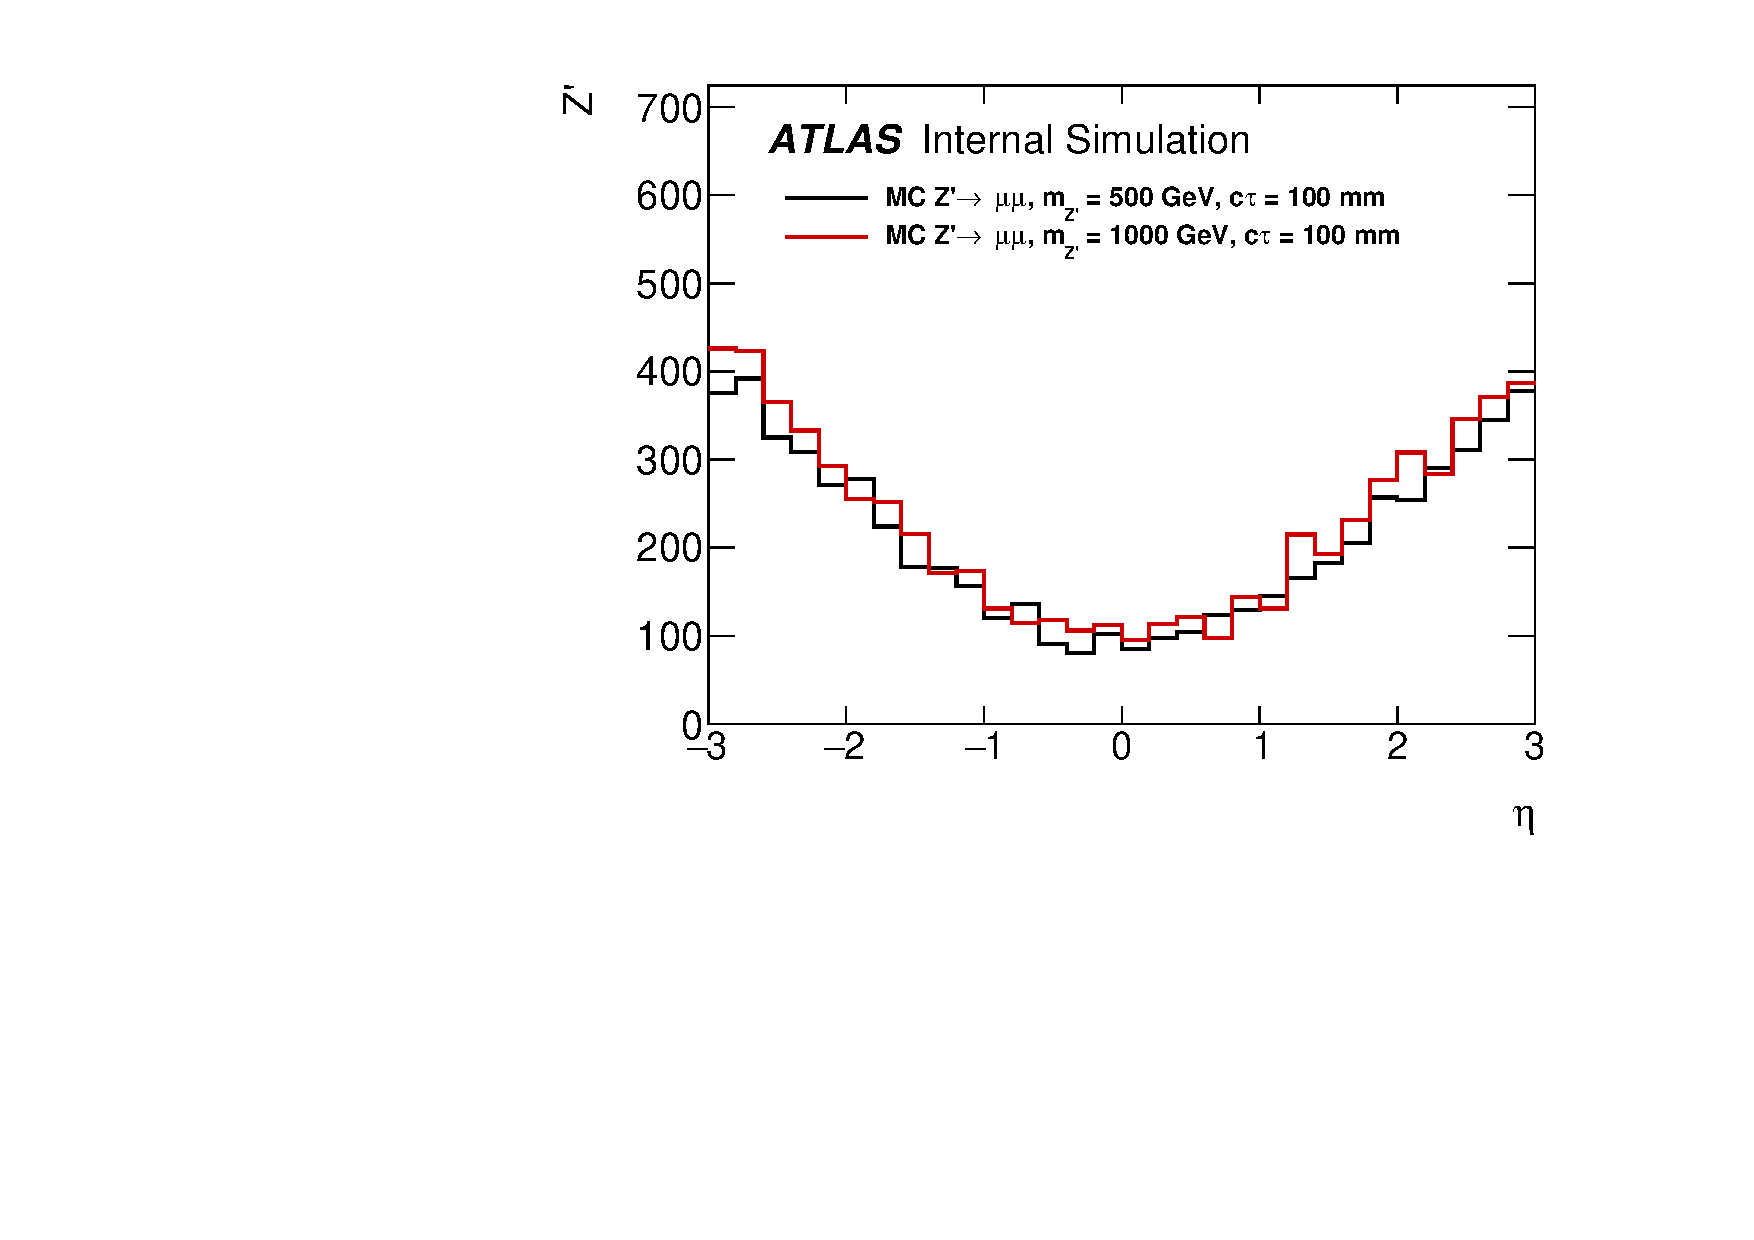
\includegraphics[width=0.45\textwidth]{figures/m_truth_zp_eta.pdf}} \\
    \subfloat[]{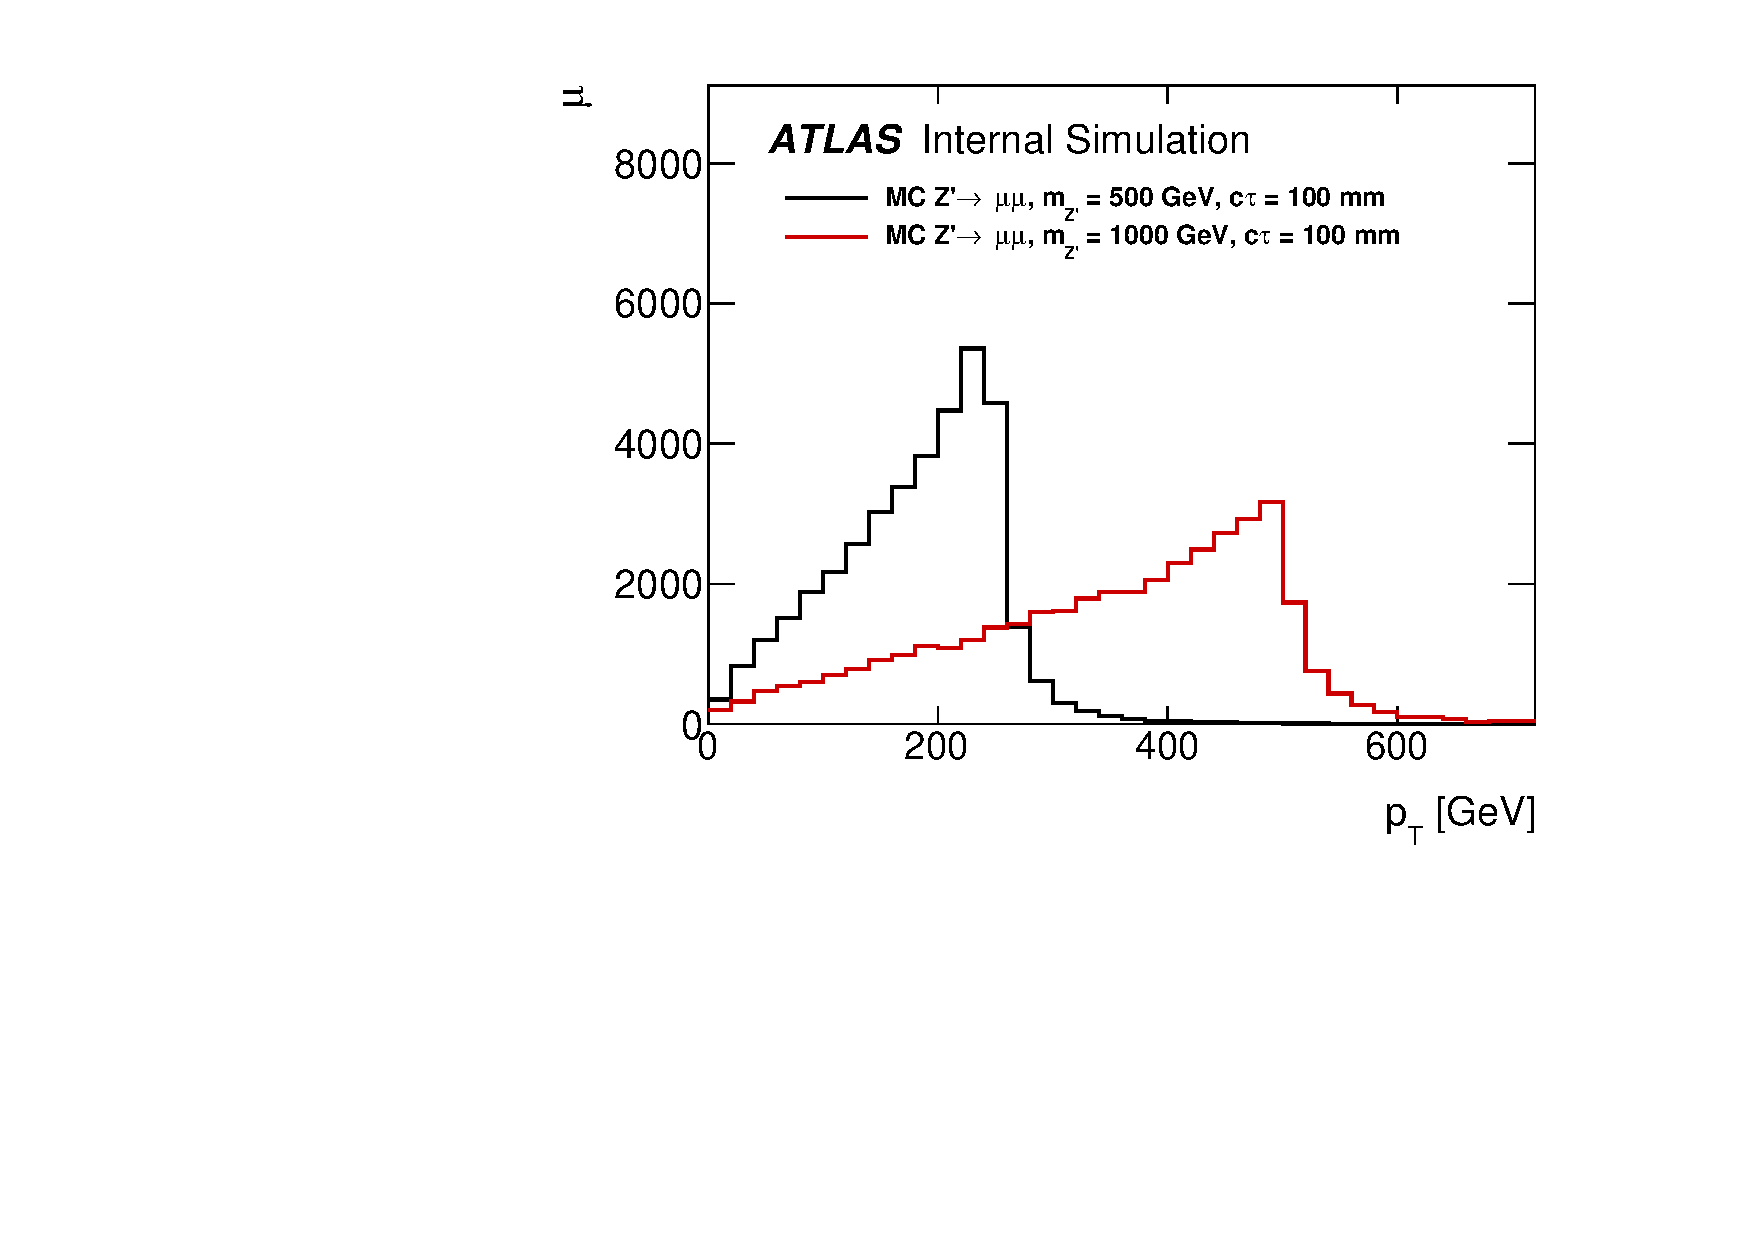
\includegraphics[width=0.45\textwidth]{figures/m_truth_muon_pt.pdf}}
    \subfloat[]{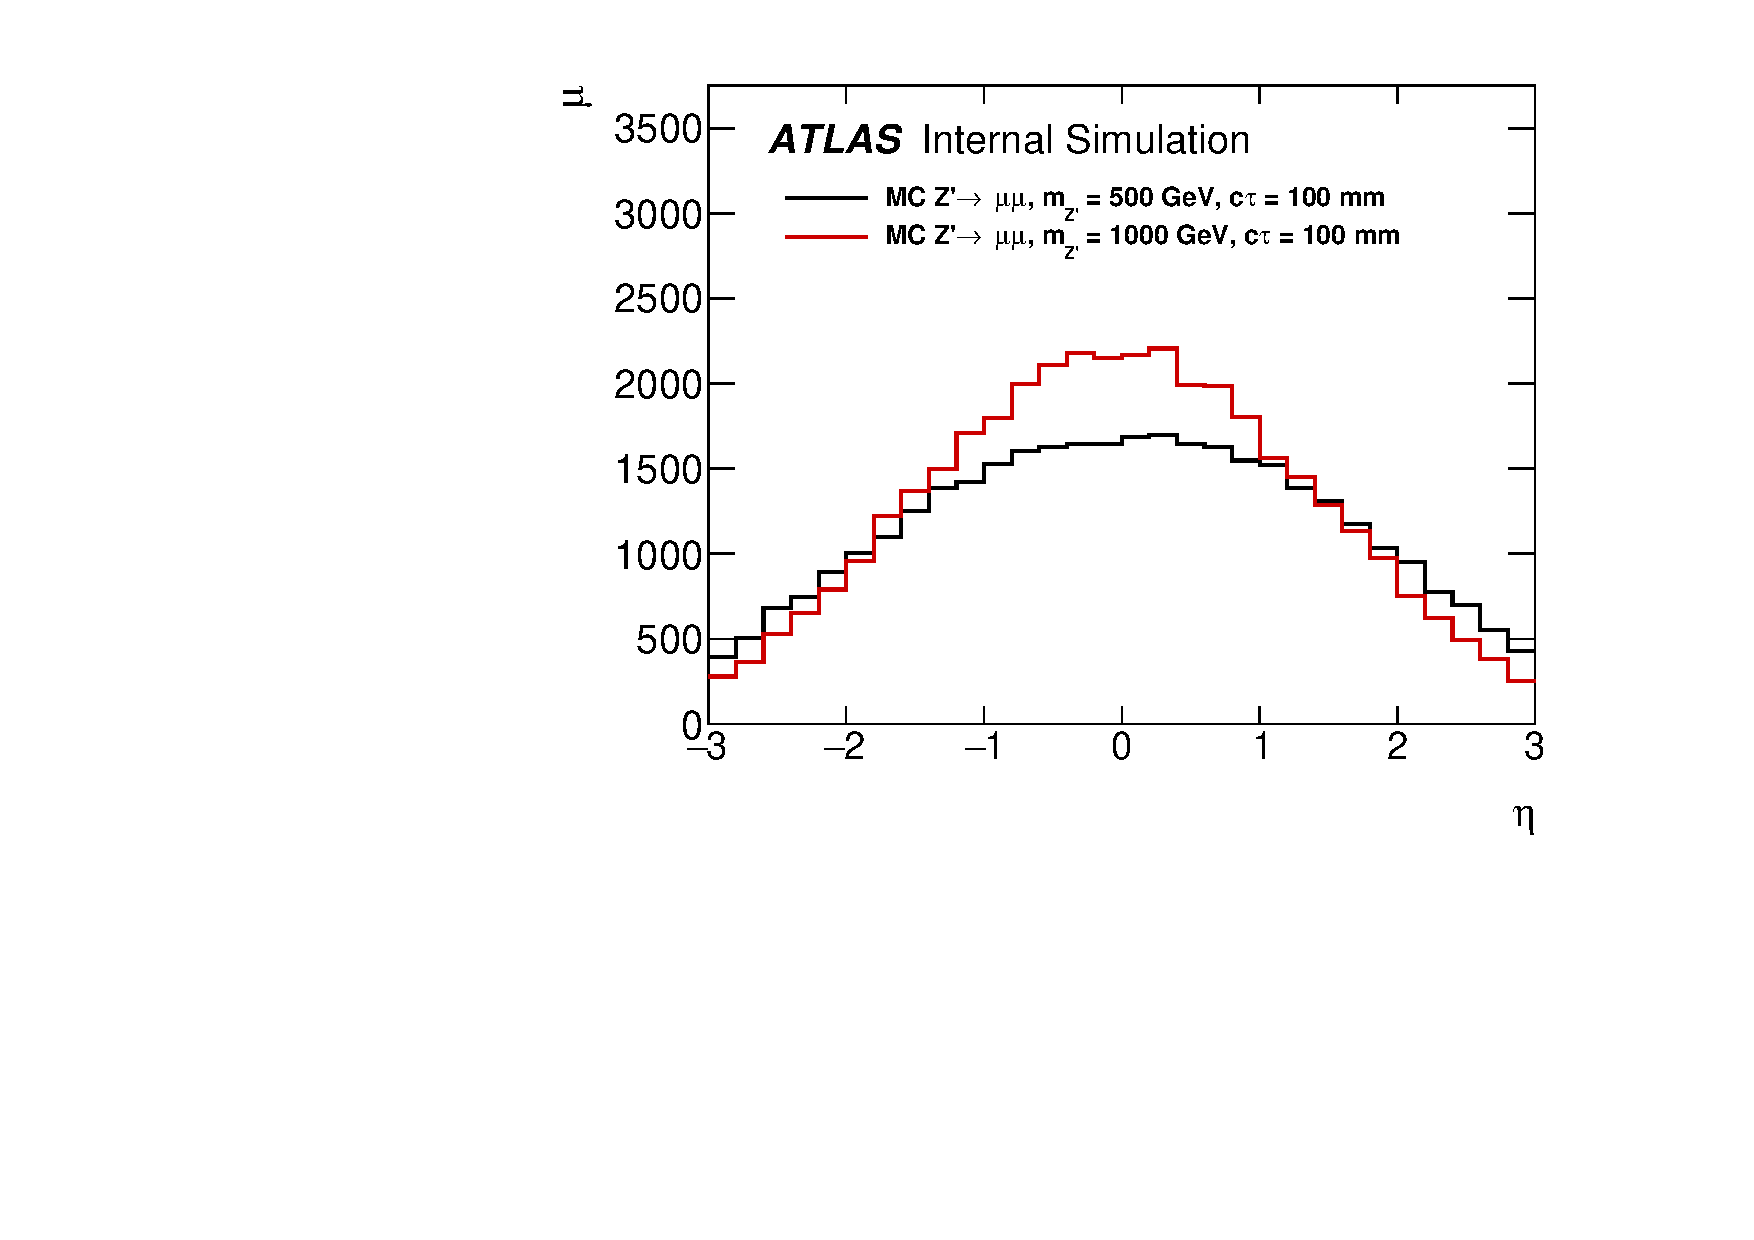
\includegraphics[width=0.45\textwidth]{figures/m_truth_muon_eta.pdf}}
    \caption{The representative plots of truth-level (a) $p_{T}$ and (b) $\eta$ distributions of $Z'$, and (c), (d) are the corresponding distributions for the signal muons. The signal MC samples are generated with $m=$ 500, 1000 GeV, and $c\tau=$ 100 mm.}
    \label{fig:truth_zp_muon}
\end{figure}


\subsubsection{Background MC samples}
\label{sec:background_mc_sample}
In this analysis, backgrounds are estimated from data because most of the backgrounds are expected to be originated from non-collision processes such as cosmic rays or random-crossing of tracks. %sources other than the SM collision process 

However, SM background samples are used to study the performance of random-crossing background estimation in Section~\ref{sec:background_estimation} and to estimate the systematic uncertainties in vertexing and tracking in Section~\ref{sec:syst}. The SM background samples are reprocessed from \texttt{HITS} using the same configuration as the signal MC sample for consistency.

The background MC samples used for background and systematic uncertainty estimations are summarized in Table~\ref{table:background_MC}.


\begin{table}[!htb]
  \centering
  \begin{tabular}{ l l l l l}
    \hline
    \hline
    Process         &   DID     &   $\sigma$ (pb)       & Events ($10^{6}$) &   $\mathcal{L}_{Int} (\mathrm{fb^{-1}})$ \\
    \hline
    $t\bar{t}$                              &   410252  &   87.8   &   0.70        &   7.97                 \\
    $ZZ\rightarrow \ell \ell \ell \ell$     &   361063  &   11.7   &   0.12        &   10.3                 \\
    $W^{-}Z\rightarrow \ell \ell \ell v$    &   361064  &   1.68   &   0.020       &   10.2                 \\
    $W^{+}Z\rightarrow \ell \ell \ell v$    &   361066  &   2.33   &   0.70        &   30.0                 \\
    $WW \rightarrow \ell \ell vv$           &   361068  &   12.8   &   0.025       &   1.95                 \\
    JZ3W                                    &   361023  &   8.45$\cdot10^{3}$      &   0.20  &   0.0247     \\
    JZ4W                                    &   361024  &   135    &   0.20        &   1.48                 \\
    JZ5W                                    &   361025  &   4.20   &   0.20        &   47.6                 \\
    JZ6W                                    &   361026  &   2.42$\cdot10^{-2}$     &   0.20  &   826        \\
    \hline
    \hline
  \end{tabular}
  \caption{Background MC samples used in the study of random-crossing background and in the estimation of tracking and vertexing systematic uncertainty.}
  \label{table:background_MC}
\end{table}


%-------------------------------------------------------------------------------
\section{Data reprocessing}
\label{sec:data_preparation}
\subsection{Event preselection}
\label{sec:preselection}
In the first step of data reprocessing, events are selected by \texttt{DRAW\_RPVLL} filters as described in Section~\ref{sec:data_MC}. The filters are designed to select events of interest while maintaining reasonably low filter rates. Single photon ($\gamma$), single electron ($e$), di-photon ($\gamma\gamma$), di-electron ($ee$), and the combination of photon and electron ($e\gamma$) filters are used to select events with $ee$ or $e\mu$ candidates of interest. Single $\mu$ filter is used to select events with $\mu\mu$ or $e\mu$ candidates of interest.

Events are required to pass one of the HLTs listed in Table~\ref{table:triggers}. In order to increase the sensitivity to electrons and muons with large transverse and longitudinal impact parameters, $d_{0}$ and $z_{0}$, the triggers with no requirement on ID tracks are used. Consequently, muon trigger with Muon Spectrometer (MS) information only and photon triggers are used.

\begin{table}[!htb]
  \centering
  \begin{tabular}{l l}
    \hline
    \hline
    Description     			& Trigger	        	                \\
    \hline
	Single photon 	            & \texttt{HLT\_g140\_loose}             \\
	Di-photon	                & \texttt{HLT\_2g50\_loose}             \\
	Single muon                 & \texttt{HLT\_mu60\_0eta105\_msonly}   \\
    \hline
    \hline
  \end{tabular}
  \caption{HLTs used to select events in \texttt{DRAW\_RPVLL} filter. Single photon trigger requires one photon with $p_{T} > 140$ GeV. Di-photon trigger requires two photons with $p_{T} > 50$ GeV. Single muon trigger requires one muon with $p_{T} > 60$ within $0 < |\eta| < 1.05$ using MS information only.}
  \label{table:triggers}
\end{table}

In addition to the HLT requirements, each filter requires offline selection on particles such as $p_{T}$, $\eta$, and $d_{0}$. Single photon ($\gamma$) or electron ($e$) filter requires a leading photon or electron, respectively, with $p_{T} > 150$ GeV, $\eta < 2.5$, and $d_{0} > 2.0$ mm. These filters also require a second photon or lepton with $p_{T} > 10$ GeV and $\eta < 2.5$ to keep the filter rate reasonably low. Single muon $\mu$ filter requires a muon with $p_{T} > 60$ GeV, $\eta < 2.5$, and $d_{0} > 1.5$ mm. Di-photon ($\gamma\gamma$), di-electron ($ee$), and the combination of photon and electron ($e\gamma$) filters require two photons/leptons with $p_{T} > 50$ GeV, $\eta < 2.5$, and $d_{0} > 2.0$ mm. The offline selection is summarized in Table~\ref{table:rpvll_filter_selection}.

\begin{table}[!htb]
  \centering
  \begin{tabular}{l c c c | c c c}
    \hline
    \hline
    Filter          & \multicolumn{3}{c|}{Leading}  &  \multicolumn{3}{c}{Second} \\
                    & $p_{T}$ (GeV) & $|\eta|$    & $d_{0}$ (mm) & $p_{T}$ (GeV) & $|\eta|$    & $d_{0}$ (mm)  \\
    \hline
    $\gamma$, $e$                   & $>$ 150   & $<$2.5  & $>$2.0  & $>$ 10 & $<$2.5 & -       \\
    $\mu$                           & $>$ 60    & $<$2.5  & $>$1.5  & -      & -      & -       \\
    $\gamma\gamma$, $ee$, $e\gamma$ & $>$ 50    & $<$2.5  & $>$2.0  & $>$ 50 & $<$2.5 & $>$ 2.0 \\
    \hline
    \hline
  \end{tabular}
  \caption{\texttt{RPVLL} filter offline selection on photon and leptons. Single photon ($\gamma$) or electron ($e$) filter requires a leading photon or electron, respectively, with $p_{T} > 150$ GeV, $\eta < 2.5$, and $d_{0} > 2.0$ mm and a second photon or lepton with $p_{T} > 10$ GeV, $\eta < 2.5$. Single muon $\mu$ filter requires a muon with $p_{T} > 60$ GeV, $\eta < 2.5$, and $d_{0} > 1.5$ mm. Di-photon ($\gamma\gamma$), di-electron ($ee$), and the combination of photon and electron ($e\gamma$) filters require a photon or lepton with $p_{T} > 50$ GeV, $\eta < 2.5$, and $d_{0} > 2.0$ mm.}
  \label{table:rpvll_filter_selection}
\end{table}

The event selected by the \texttt{RPVLL} filters are passed downstream as \texttt{DRAW\_RPVLL} for the special track and vertex reconstruction.


\subsection{Reconstruction}
\label{sec:track_vertex_reconstruction}

\subsubsection{Large radius tracking}
\label{sec:large_radius_tracking}

The standard track reconstruction in ATLAS is optimized\footnote{There are dedicated algorithms for reconstructing displaced decays such as photon conversion and $b$-hadron decays, but their usage is limited to the particular topologies.} for the reconstruction of particles that are originating from the primary $pp$ interaction point (IP). The requirements on $d_{0}$ and $z_{0}$ limit the tracking efficiency at large impact parameters ($d_{0}$ > 2 mm). To improve the tracking efficiency at large impact parameter, the large radius tracking algorithm is used for track reconstruction.

The large radius tracking is performed as the third tracking sequence following the standard \textit{inside-out} and \textit{outside-in} track reconstruction~\cite{Cornelissen:1020106}. It follows the similar track reconstruction strategy as the standard \textit{inside-out} track reconstruction, but there are a few important differences between the two tracking algorithms.

\begin{itemize}
	\item The large radius tracking only uses un-used hits from the standard \textit{inside-out} and \textit{outside-in} track reconstruction for track seed creation.
	\item The requirements on tracks such as $d_{0}$, $z_{0}$, and number of hits are relaxed.
\end{itemize}

The track requirements in the standard track reconstruction and the large radius tracking are compared in Table~\ref{table:lrt_comparison}. More details on the large radius tracking can be found in Ref.~\cite{Che:2255680}.

\begin{table}[!htb]
  \centering
  \begin{tabular}{ l  c  c } 
    \hline
    \hline
    & Standard & Large radius \\ [0.5ex] 
    \hline
    Maximum $d_{0}$ (mm) & 10 & 300 \\ 
    Maximum $z_{0}$ (mm) & 250 & 1500 \\
    % $\sigma_{d0}$ & - & - \\
    %$\sigma_{z0}$ & - & - \\
    Maximum $|\eta|$ & 2.7 & 5 \\
    Maximum shared silicon modules & 1 & 2 \\
    Minimum unshared silicon hits& 6 & 5 \\
    Minimum silicon hits & 7 & 7\\
    Seed extension & Combinatorial & Sequential \\
    \hline
    \hline
  \end{tabular}
  \caption{Comparison of track requirements between the standard and large radius trackings.}
  \label{table:lrt_comparison}
\end{table}

The collection of tracks reconstructed by the large radius tracking, referred as \textit{large radius tracks}, is merged with the track collection from the standard track reconstruction. The combined track collection is used as an input for the lepton reconstruction and identification and secondary vertex reconstruction.

\subsubsection{Lepton reconstruction and identification}
\label{sec:lepton_reconstruction}

In this search, the standard ATLAS electron and muon reconstruction and identification algorithms are used. The combined track collection, including both standard and large radius tracks, is used as an input. Therefore, standard muon or electron working points such as \texttt{Tight}, \texttt{Medium}, or \texttt{Loose} are available after the lepton identification. A few changes are implemented in the muon reconstruction algorithm to improve the muon reconstruction efficiency at large impact parameters;

\begin{itemize}
	\item requirements on $d_{0}$ and Pixel hits of muon tracks are removed.
	\item minimum SCT hits on muon tracks are lowered to 2.
\end{itemize}

Details of these algorithms are discussed in Refs.~\cite{ATLAS-CONF-2010-005} and~\cite{Aad:2016jkr}.

\subsubsection{Secondary vertex reconstruction}
\label{sec:secondary_vertex_reconstruction}

Secondary vertices are reconstructed by \texttt{VrtSecInclusive} algorithm. The algorithm was originally developed for the material mapping of the ID in Run I, but updated for several long-lived particle searches in Run 2.

The secondary vertex reconstruction starts by selecting tracks that satisfy the requirements on track parameters and hit patterns as shown in Table~\ref{table:vertex_track_selection_simple}. Both large radius tracks and standard tracks are used as input, and tracks passing the requirements are stored for the next step of the vertex reconstruction.

\begin{table}[!htb]
  \centering
  \begin{tabular}{ l c }
    \hline
    \hline
	Variable      		& Cut                                         	\\
    \hline
	$p_{T}$ (GeV)		& $>$ 1.0										\\
	$\chi^{2} / DOF$	& $<$ 50.0										\\
	$d_{0}$	(mm)		& 2.0 - 300.0									\\
	$z_{0}$ (mm)		& $<$ 1500.0									\\
	SCT hits			& $\geq$ 2										\\
	Si shared hits	    & $\leq$ 2										\\
	Pixel and TRT hits  & TRT hits > 0 or Pixel hits $\geq$ 2			\\
    \hline
    \hline
  \end{tabular}
  \caption{Track requirements for secondary vertex reconstruction.}
  \label{table:vertex_track_selection_simple}
\end{table}

The selected tracks are used for the creation of two-track \textit{seed} vertices. From the \textit{seed} vertices, fake vertices are rejected by considering the location of a vertex and hit patterns of the tracks from the vertex. Tracks are not allowed to have any hits at radius smaller than the vertex position. \textit{seed} vertices passing the location and hit patterns requirement are used to create N-track vertices. Ambiguity solving is applied to N-track vertices to improve the purity of the reconstructed vertices. More details of the algorithm can be found in Ref.~\cite{ATLAS-CONF-2010-058}.

The two-track secondary vertices reconstructed by \texttt{VrtSecInclusive} is the primary analysis object, and Section~\ref{sec:vertex_selection} discuss the vertex selection applied to these two-track vertices to select displaced vertices. Lepton identification requirements are applied to the tracks from secondary vertices after applying analysis level vertex selection, so secondary vertices reconstructed can have any combination of muon, electron, or non-leptonic tracks.



%-------------------------------------------------------------------------------
\section{Signal selection}
\label{sec:signal_selection}
%Events are pre-selected with \texttt{RPVLL} filters, and the selected events are reprocessed with a special setup so that large radius tracks and secondary vertices are reconstructed as described in Section~\ref{sec:data_preparation}.
In this section, the analysis level selections applied to events, leptons, and and vertices are described.

\subsection{Event selection}
\label{sec:event_selection}
%Events are selected by minimum requirements on the quality of events, completeness of luminosity blocks, and HLTs used in this analysis. The event selections are as follows.
Minimum requirements are placed on events based on the quality of events, completeness of the corresponding luminosity blocks, primary vertex, and HLTs used in this analysis. In addition, cosmic veto is applied to reject events with back-to-back muons. The event selection is described below.

\begin{itemize}
    \item \texttt{GoodRunsList} removes events from incomplete luminosity blocks.
    \item Event cleaning removes corrupted/bad events due to problems in TileCal, LAr noise bursts, SCT recovery, or TTC restarts~\cite{ElectronPhotonRun2}.
    \item Events are required to pass one of the HLTs listed in Table~\ref{table:triggers}.
    \item Events are required to have at least one primary vertex along the beam line ($z<200$ \si{\mm}).
    \item Events are rejected if there is a pair of leptons with $R_{\mathrm{CR}} < 0.01$ where $R_{\mathrm{CR}} = \sqrt{(\Delta \phi - \pi)^{2} + (\Sigma \eta)^{2}}$.
\end{itemize}

The event selection is summarized in Table~\ref{table:signal_selection}.

\subsection{Muon and electron requirements}
\label{sec:muon_electron_selection}
Prior to applying the vertex level selections, tracks from vertices are required pass the requirements on kinematics, overlap removal, and muon and electron identification criteria.

Electron requirements are based on the recommendations from EGamma group~\cite{ElectronPhotonRun2} with a few optimization for electrons with large impact parameters. Electrons are rejected if there is a bad cluster associated with an electron. Basic kinematic cuts are applied to electrons, $|\eta| < 2.47$ and $p_{T}$ > 7 GeV. The electron \texttt{LooseLH} working point is used, but the requirements on $d_{0}$ and Pixel hits are removed to improve electron detection efficiency at large impact parameters.

Muon requirements are based on the recommendations from MuonCombinedPerformance group~\cite{MuonRun2}. Muon \texttt{Loose} working point is used for the identification criteria, and a fiducial cut, $|\eta| < 2.5$, and kinematic cut, $p_{T}$ > 10 GeV, are applied to muons. The requirements on Pixel hits are removed to improve muon detection efficiency at large impact parameters. In addition, muons are required to be \texttt{CombinedMuons} to ensure that they have associated ID tracks for vertex reconstruction. In case of MC samples, muon momentum resolution and scale correction are applied to the simulated muons for better agreement between data and simulation~\cite{Aad:2016jkr}. 

Overlap removal is applied to both muons and electrons to ensure that a ID track is associated with only one muon or electron.%Muons or electrons are removed from vertices if they do not pass the muon or electron requirements.
The muon and electron requirements are summarized in Table~\ref{table:lepton_requirement}.

\begin{table}[!htb]
  \centering
  \begin{tabular}{ l  l }
    \hline
    \hline
    \textbf{Muon}     &       Overlap removal                                                             \\
                                  &       Muon \texttt{Loose}                                                         \\
                                  &       $|\eta| < 2.5$                                                           \\
                                  &       $p_{T} > 10.0$ GeV                                                       \\
                                  &       Combined Muon                                                            \\
    \hline
    \textbf{Electron} &       Overlap removal                                                             \\
                                  &       Bad cluster removal                                                         \\
                                  &       Electron \texttt{LooseLH} (no requirement related to $d_{0}$, Pixel hits)   \\
                                  &       $|\eta| < 2.47$                                                             \\
                                  &       $p_{T} > 7.0$ GeV                                                           \\
    \hline
    \hline
  \end{tabular}
  \caption{Muon and electron requirements applied at analysis level.}
  \label{table:lepton_requirement}
\end{table}

\subsection{Vertex selection}
\label{sec:vertex_selection}
The vertex selection is applied to two-track secondary vertices found in Section~\ref{sec:secondary_vertex_reconstruction}. Secondary vertices with minimum displacement of 2 mm from the primary vertex are selected. The selected displaced vertices are made of two tracks which can be any combination of muon, electron, and non-lepton tracks. Therefore, vertices are separated into three vertex types, control, validation, and signal regions.

In the control region, vertices are required to have two non-leptonic tracks (xx). In the validation region, vertices are required to have a muon or an electron and another non-leptonic track ($\mu$x, $e$x). In signal region, vertices are required to have a muon pair, an electron pair, or a muon-electron pair ($\mu\mu$, $ee$, $e\mu$). The control region and the validation region are used for background (Section~\ref{sec:background_estimation}) and systematic uncertainty (Section~\ref{sec:syst}) estimations. The control, validation, and signal regions are summarized in Table~\ref{table:vertex_type}.

\begin{table}[!h]
  \centering
  \begin{tabular}{ l  c}
    \hline
    \hline
	Region				& Vertex Type										\\
    \hline
	Control     		& xx $xx$   										\\
	Validation       	& $\mu$x, $e$x										\\
	Signal       		& $\mu\mu$, $ee$, $e\mu$							\\
    \hline
    \hline
  \end{tabular}
  \caption{The control, validation, and signal regions defined by the vertex type.}
  \label{table:vertex_type}
\end{table}

In all regions, vertices are required to pass a common set of vertex selections described as follows. Vertices are required to have $\chi^2 / \mathrm{ DOF} <$ 5 to reject poorly reconstructed vertices. A minimum transverse displacement of 2 mm from the primary vertex is required to suppress background from prompt decays. Two tracks from a vertex are required to have opposite charges. Vertices are rejected if they are within the volume of disabled Pixel module~\cite{Backhaus:2110260}. Hadronic interaction of charged particles with detector material is a major source of backgrounds. Therefore, the vertices are rejected if they are within dense detector material~\cite{Aaboud:2016poq}. The material veto is not applied to $\mu\mu$ type vertex due to low probability of muon interaction with detector material. Vertices are also required to be in the detector volume covered by the material mapping ($r < 300$ \si{mm}, $z < 300$ \si{mm}). The vertices are required to have $m >$ 10 GeV to suppress backgrounds from low mass SM particles such as $J/\Psi$. The vertex mass is calculated by the secondary vertex reconstruction algorithm with the assumption that all tracks have pion mass. Cosmic veto is applied to vertices by requiring $R_{\mathrm{CR}} > 0.01$. The cosmic veto is very effective in rejecting cosmic muons reconstructed as back-to-back muon vertices, and the details are discussed in Section~\ref{sec:cosmic_ray}

In addition to the common vertex selection, at least one electron or muon from the vertex is required to be matched with one of the triggers listed on Table~\ref{table:triggers} and the filters listed on Table~\ref{table:rpvll_filter_selection} in the signal region. The vertex selection is summarized in Table~\ref{table:signal_selection}.

\begin{table}[!htb]
  \centering
  \begin{tabular}{ l  l }
    \hline
    \hline
    \textbf{Event}           &       GoodRunsList (Section~\ref{sec:preselection})                               \\
                             &       Trigger filter (Section~\ref{sec:preselection})                             \\
                             &       Event cleaning (Section~\ref{sec:event_selection})                          \\
                             &       Cosmic veto    (Section~\ref{sec:event_selection})                          \\
                             &       $z_{\mathrm{PV}} < 200$ mm (Section~\ref{sec:event_selection})                       \\
    \hline
    \textbf{Vertex}&       Trigger matching (signal region only)                                          \\
                             &       $\chi^2 / \mathrm{ DOF} < 5$                                                \\
                             &       $r > $2 mm                                                           \\
                             &       Opposite charge                                                             \\
                             &       Disabled module veto                                                        \\
                             &       Material veto (excluding $\mu\mu$)                                                              \\
                             &       $m > 10$ GeV                                                                \\
                             &       $R_{\mathrm{CR}} > 0.01$                                                    \\
                             &       $r < 300$ \si{mm}, $z < 300$ \si{mm}                                        \\
                             &       Filter matching (signal region only)                                                            \\
    \hline
    \hline
  \end{tabular}
  \caption{Event and vertex selections applied to select displaced vertices.}
  \label{table:signal_selection}
\end{table}




%-------------------------------------------------------------------------------
\section{Signal efficiency}
\label{sec:signal_efficiency}
The signal efficiency of finding displaced dilepton vertex is defined by the ratio of the number of events passing the signal selection (Section~\ref{sec:signal_selection}) to the total number of events processed. The signal efficiency can be written as Eq.~\ref{eq:OverallEff}. 

\begin{equation}
\label{eq:OverallEff}
\varepsilon_{\mathrm{overall}} = \varepsilon_{\mathrm{filter}} \cdot \varepsilon_{\mathrm{trigger}} \cdot 
                     (\varepsilon_{\mathrm{tracking}} \cdot \varepsilon_{\mathrm{leptonID}})^2 \cdot
                     (\varepsilon_{\mathrm{vertexTrack}})^2 \cdot
                     \varepsilon_{\mathrm{vertexFit}}.
\end{equation}

$\varepsilon_{\mathrm{filter}}$ and $\varepsilon_{\mathrm{trigger}}$ together represent the efficiency of \texttt{RPVLL} filter, the ratio of the events passing \texttt{RPVLL} filter to the total events processed. \texttt{RPVLL} filter has the trigger filter as one of its requirements, and because it is desirable to study the trigger efficiency independently from the filter efficiency, \texttt{RPVLL} filter efficiency is factorized into the filter efficiency and the trigger efficiency. $\varepsilon_{\mathrm{tracking}}$ represents the efficiency to reconstruct ID tracks from signal particles, and $\varepsilon_{\mathrm{leptonID}}$ represents the efficiency to identify the signal particles with reconstructed ID tracks as leptons. $\varepsilon_{\mathrm{vertexTrack}}$ represents the efficiency for the reconstructed signal leptons to be selected for secondary vertex reconstruction, and $\varepsilon_{\mathrm{vertexFit}}$ represents the efficiency to reconstruct a displaced vertex using two signal leptons and pass the vertex selection.
%Therefore, $\varepsilon_{\mathrm{filter}}$ is defined by the fraction of events passing \texttt{RPVLL} filter requirements without the trigger filter, and $\varepsilon_{\mathrm{trigger}}$ is defined by the fraction of events passing one of the HLTs used in this search.

In order to understand the source of signal efficiency loss, the trigger efficiency is studied in Section~\ref{sec:trigger_efficiency}, and the tracking and lepton identification efficiencies are studied in Section~\ref{sec:tracking_efficiency}.

\section{Trigger efficiency}
\label{sec:trigger_efficiency}
The trigger efficiency is defined as the ratio of the events passing one of the triggers used in this analysis to the total events processed. No \texttt{RPVLL} filter is applied when estimating the trigger efficiency.

The analysis uses three triggers listed on Table~\ref{table:triggers} to select the events with displaced dilepton vertex candidates. The single muon trigger is sensitive to the events with a $\mu\mu$ or $e\mu$ vertex. The di-photon trigger is mainly used select the events with an $ee$ vertex, but a small number of events with an $e\mu$ vertex pass this trigger. The single photon trigger is sensitive to the events with $ee$ or $e\mu$ vertex, but its efficiency is relatively low in comparison with the other two triggers.

 Figure~\ref{fig:m_trig_eff_allchannel} shows the efficiency of each trigger and the combined trigger efficiency on the signal MC samples of $Z'$ decaying to all three channels at $m = $ 250 GeV and $c\tau=$ 250 mm. The sample with $ee$ channel shows the highest combined trigger efficiency due to the high efficiency in di-photon trigger, and the sample with $e\mu$ channel shows the reduced combined trigger efficiency because $e\mu$ vertices have only one track that can satisfy either the single muon or photon trigger.

\begin{figure}[!htb]
	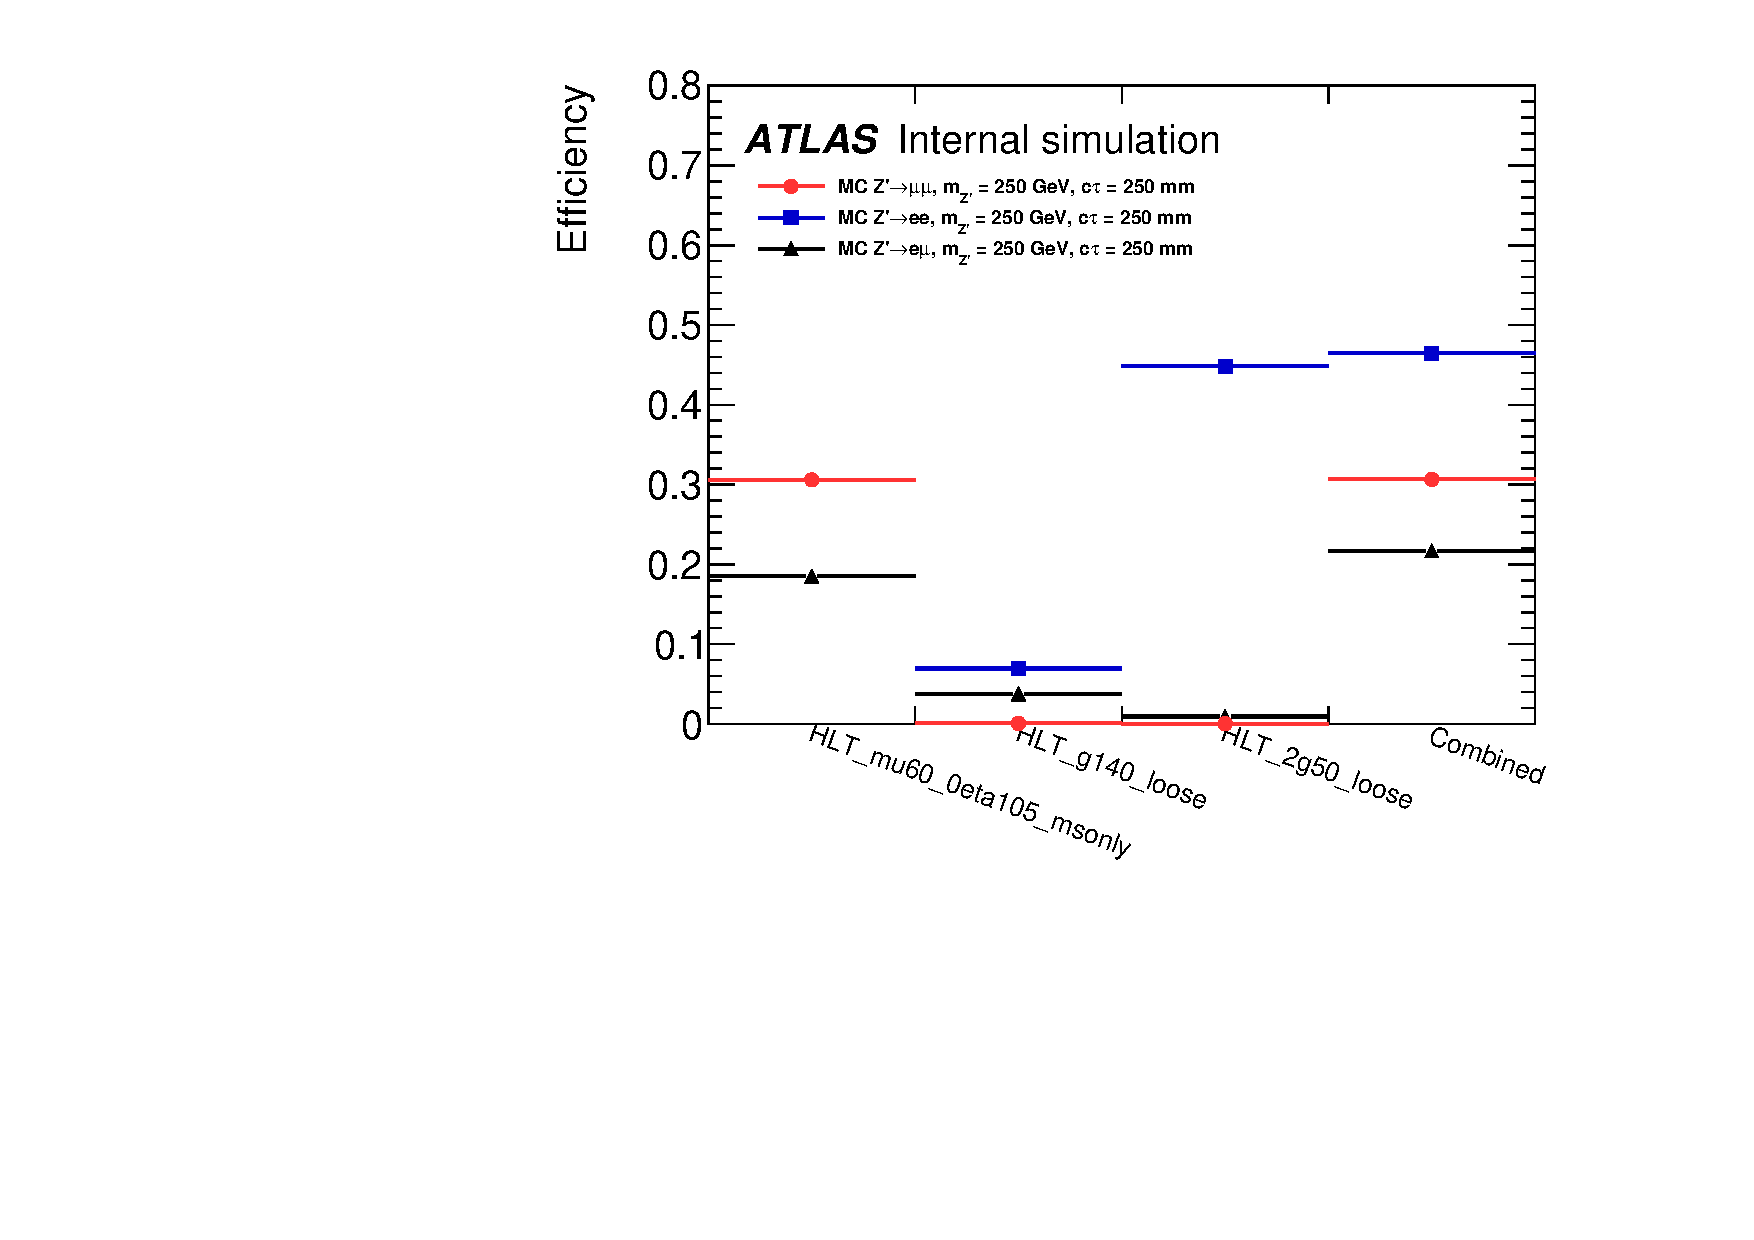
\includegraphics[width=0.50\textwidth]{figures/m_dv_eff_trig_allchannel.pdf}
	\centering
	\caption{Trigger efficiency of single muon, single photon, di-photon, and the combined triggers of the signal MC samples of $Z'\rightarrow\mu\mu, ee$, and $e\mu$ generated with $m=$ 250 GeV and $c\tau=$ 250 mm.}
	\label{fig:m_trig_eff_allchannel}
\end{figure}

The trigger efficiency on all $\mu\mu$ signal MC samples is shown in Table~\ref{table:m_trig_eff_mumu}. It is evident that at low $Z'$ mass ($\backsim$100 GeV), the combined trigger efficiency on the signal MC sample is significantly reduced because the typical $p_{T}$ of the signal muons is lower than the $p_{T}$ threshold of the single muon trigger.

The trigger study indicates that there is a substantial loss in the signal efficiency at trigger level before reconstruction, and developing dedicated, more efficient triggers for long-lived particles will provide potential improvement in sensitivity to long-lived particles. The systematic uncertainties in trigger efficiency is estimated by tag-and-probe method in Section~\ref{sec:syst_trigger}.

\begin{table}[!htb]
  \centering
  \begin{tabular}{ c c | c c c c}
    \hline
    \hline
    %       &       & \multicolumn{4}{c}{$Z'\rightarrow\mu\mu$}                \\
    $m_{Z'}$ (GeV) & $c\tau$ (mm) & Single muon & Single photon & Di-photon & Combined \\
    \hline
    100			&	100	& 0.047 	& < 0.001   &0  	    &0.047  		\\
    100			&	250	& 0.043  	&0  	 	&0  	    &0.043  		\\
    100			&	500	& 0.039 	&0  	 	&0  	    &0.039  		\\
    250			&	100	& 0.343  	&< 0.001 	&< 0.001    &0.344  		\\
    250			&	250	& 0.306  	&< 0.001 	&< 0.001    &0.307  		\\
    250			&	500	& 0.230 	&< 0.001 	&< 0.001    &0.230  		\\
    500			&	100	& 0.454 	&0.010   	&< 0.001    &0.459  		\\
    500			&	250	& 0.410 	&0.009   	&< 0.001    &0.415  		\\
    500			&	500	& 0.331  	&0.008   	&0.001      &0.336  		\\
    750			&	100	& 0.541 	&0.026   	&0.002      &0.553  		\\
    750			&	250	& 0.470 	&0.023   	&0.003      &0.481  		\\
    750			&	500	& 0.391 	&0.022 	    &0.001      &0.402  		\\
    1000	    &	100	& 0.570   	&0.039   	&0.004      &0.586  		\\
    1000	    &	250	& 0.512   	&0.036   	&0.003      &0.526  		\\
    1000	    &	500	& 0.430   	&0.034 	    &0.004      &0.444  		\\
    \hline
    \hline
  \end{tabular}
  \caption{Trigger efficiency of single muon, single photon, di-photon triggers, and the combined trigger efficiency on the signal MC samples of $Z'\rightarrow\mu\mu$.}
  \label{table:m_trig_eff_mumu}
\end{table}

\section{Lepton reconstruction efficiency}
\label{sec:tracking_efficiency}
The tracking efficiency, $\varepsilon_{\mathrm{track}}$, and the lepton identification efficiency, $\varepsilon_{\mathrm{leptonID}}$, are studied together as a lepton reconstruction efficiency. The lepton reconstruction efficiency is defined and estimated as follows. From a signal MC sample, the leptons decaying from $Z'$ are collected at truth-level, referred as \textit{truth} signal leptons. For each truth signal lepton, if there is a reconstructed lepton with its ID track matched to the ID track of the truth signal lepton by a hit-based truth matching scheme, it is marked as reconstructed. The ratio of reconstructed signal leptons to the total number of signal leptons produced in the sample is taken as the lepton reconstruction efficiency. No \texttt{RPVLL} or trigger filter is applied in estimating the lepton reconstruction efficiency.

Figure~\ref{fig:lepton_eff} shows the representative plot of the lepton reconstruction efficiency as a function of track parameters using the combined signal MC samples of $Z'$ decaying to all three channels, generated with $m = $ 250 GeV and $c\tau=$ 250 mm.

\begin{figure}[!htb]
    \centering
    \subfloat[]{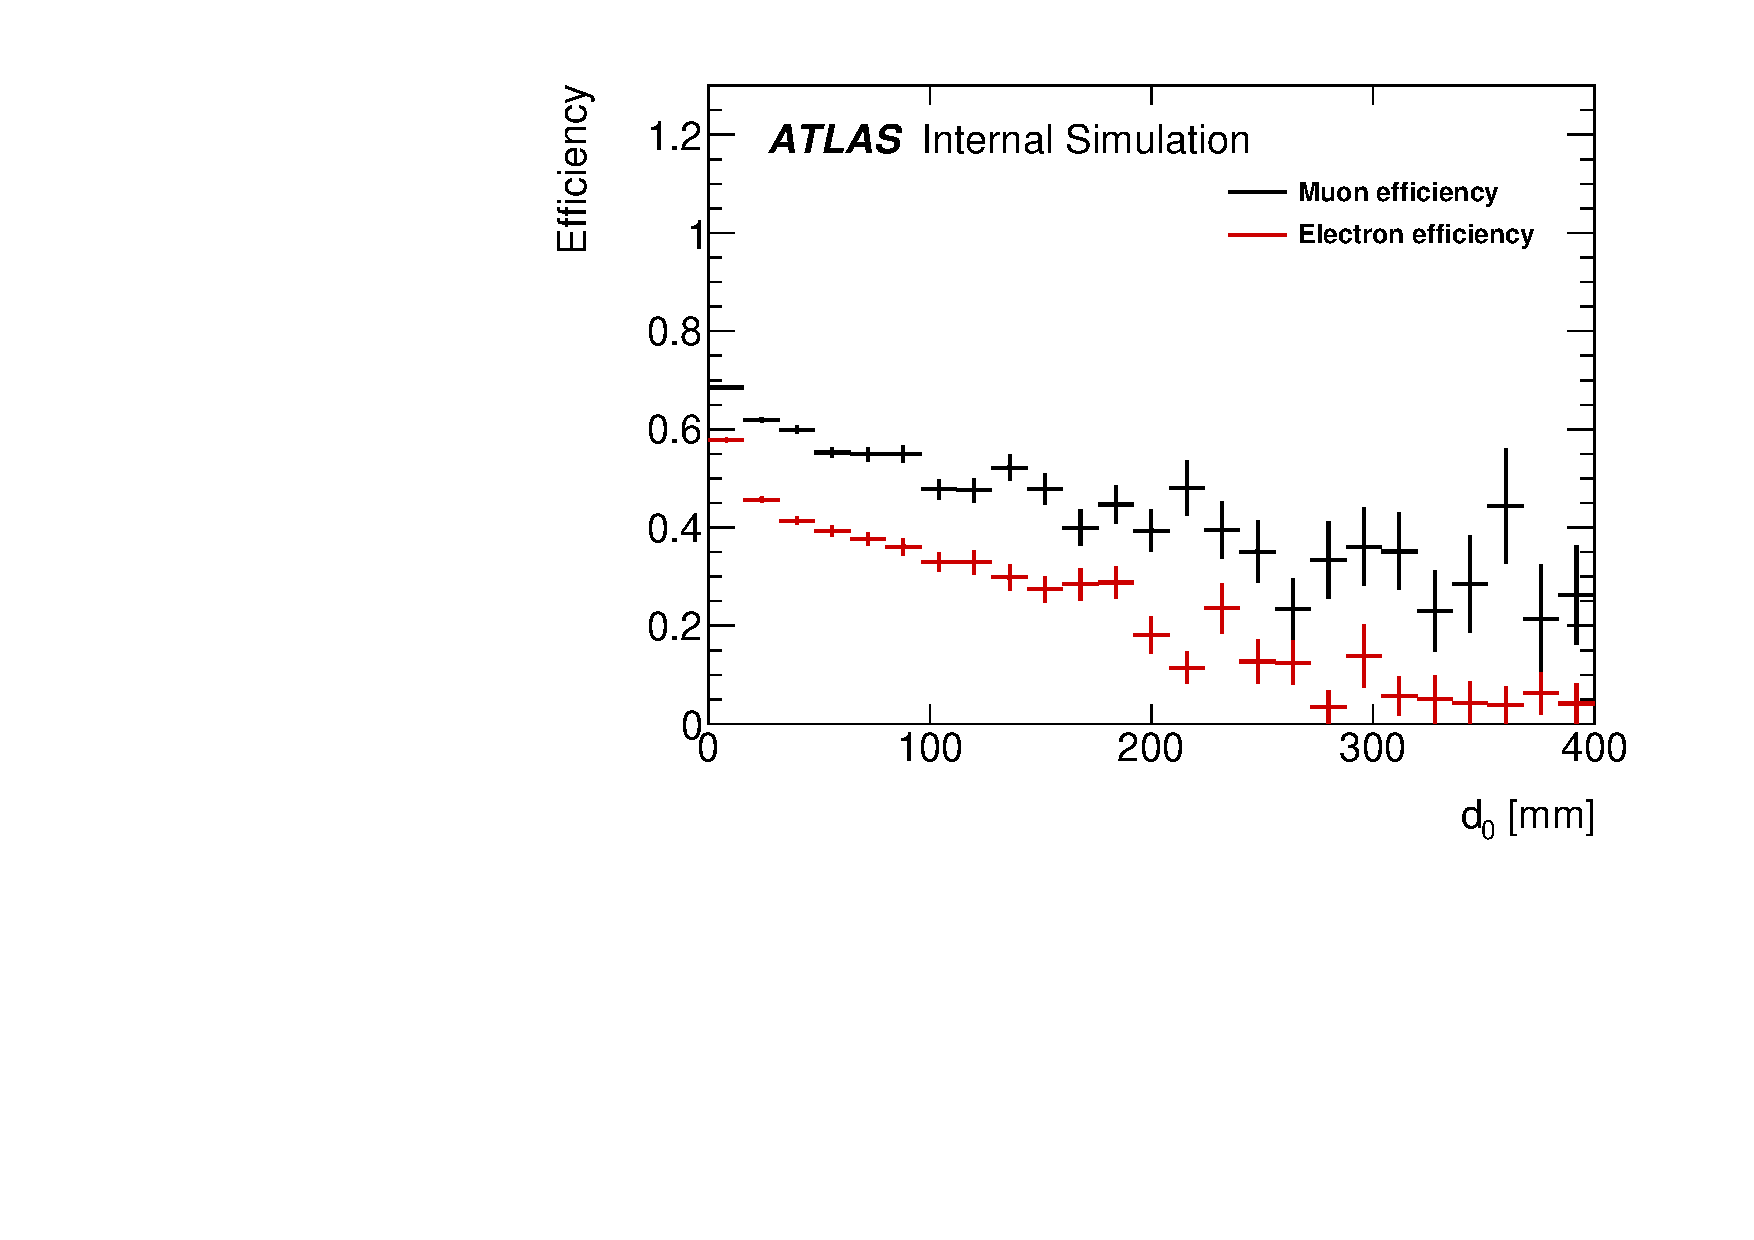
\includegraphics[width=0.50\textwidth]{figures/m_lepton_efficiency_d0.pdf}}
    \subfloat[]{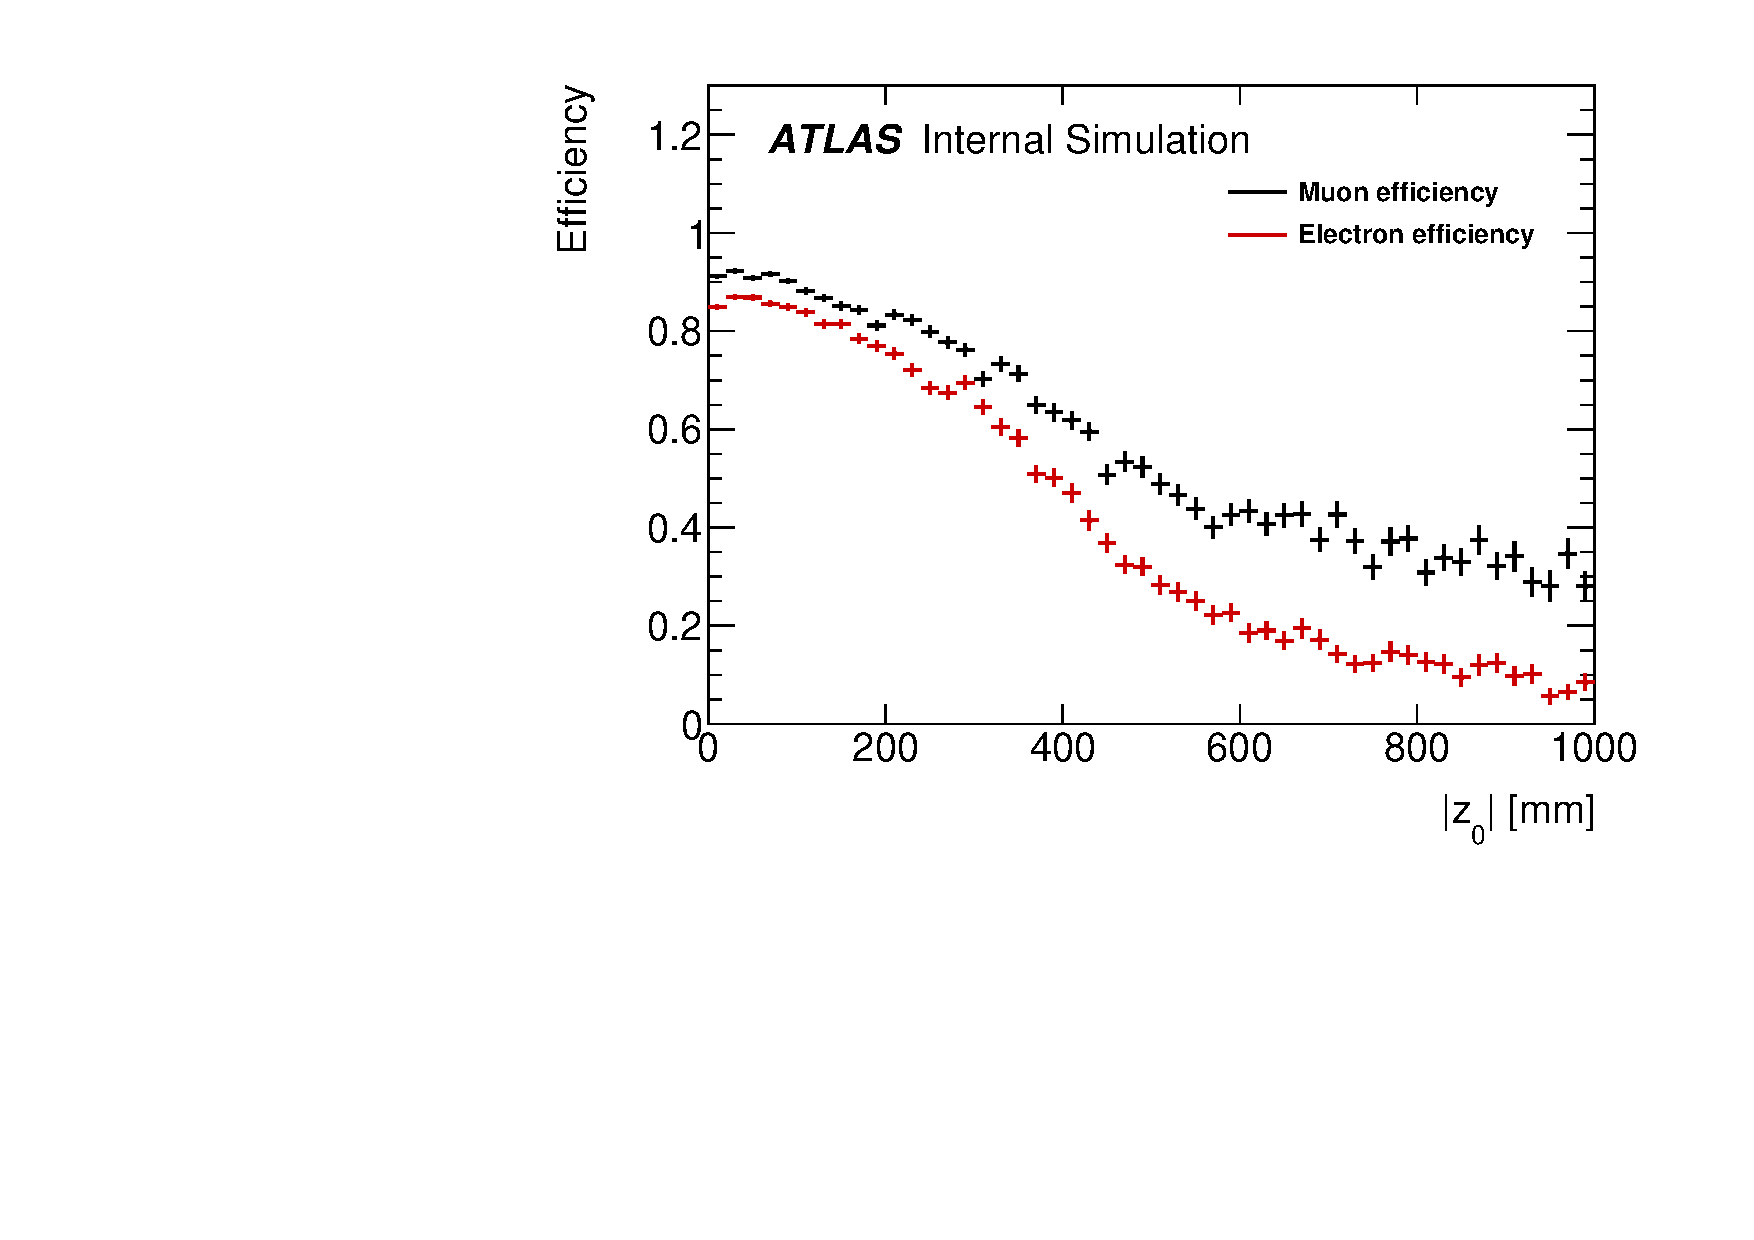
\includegraphics[width=0.50\textwidth]{figures/m_lepton_efficiency_z0.pdf}} \\
    \subfloat[]{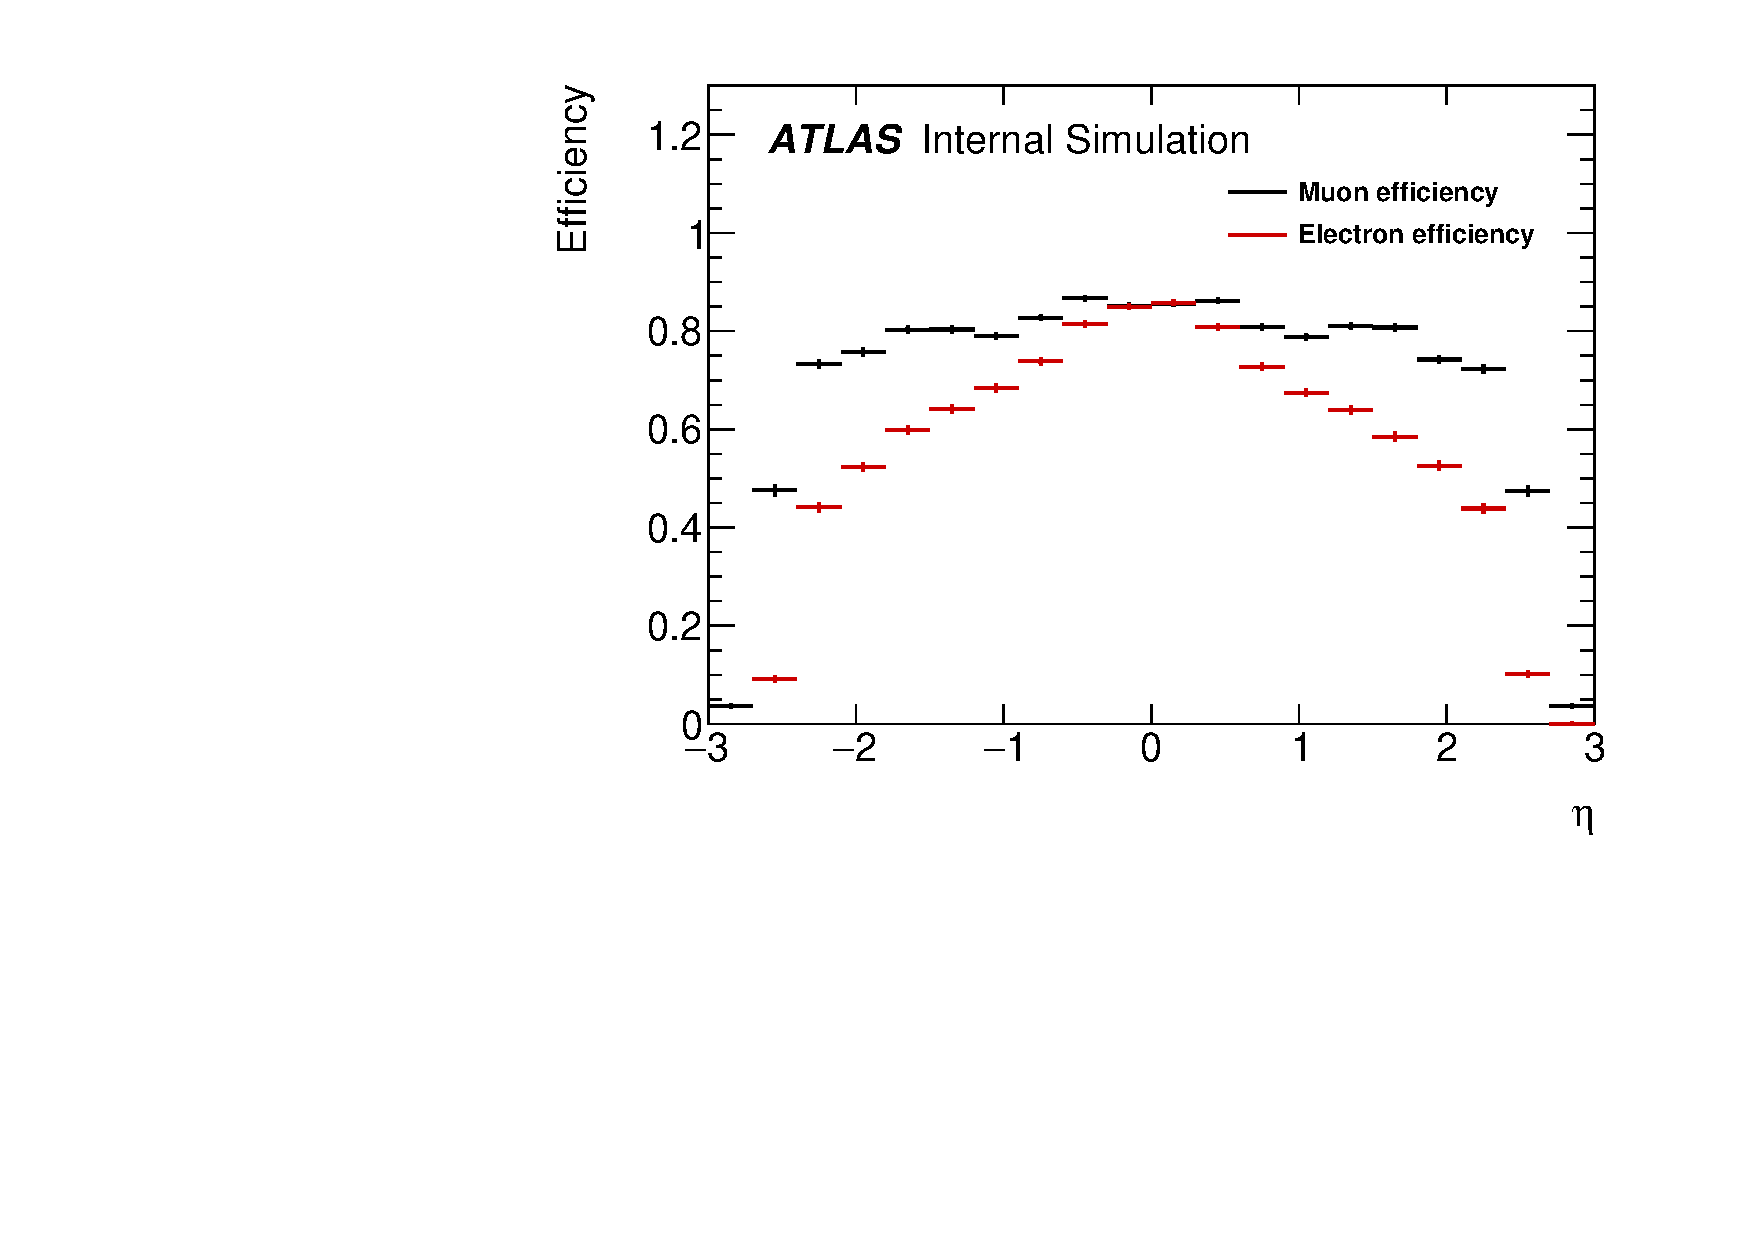
\includegraphics[width=0.50\textwidth]{figures/m_lepton_efficiency_eta.pdf}}
    \subfloat[]{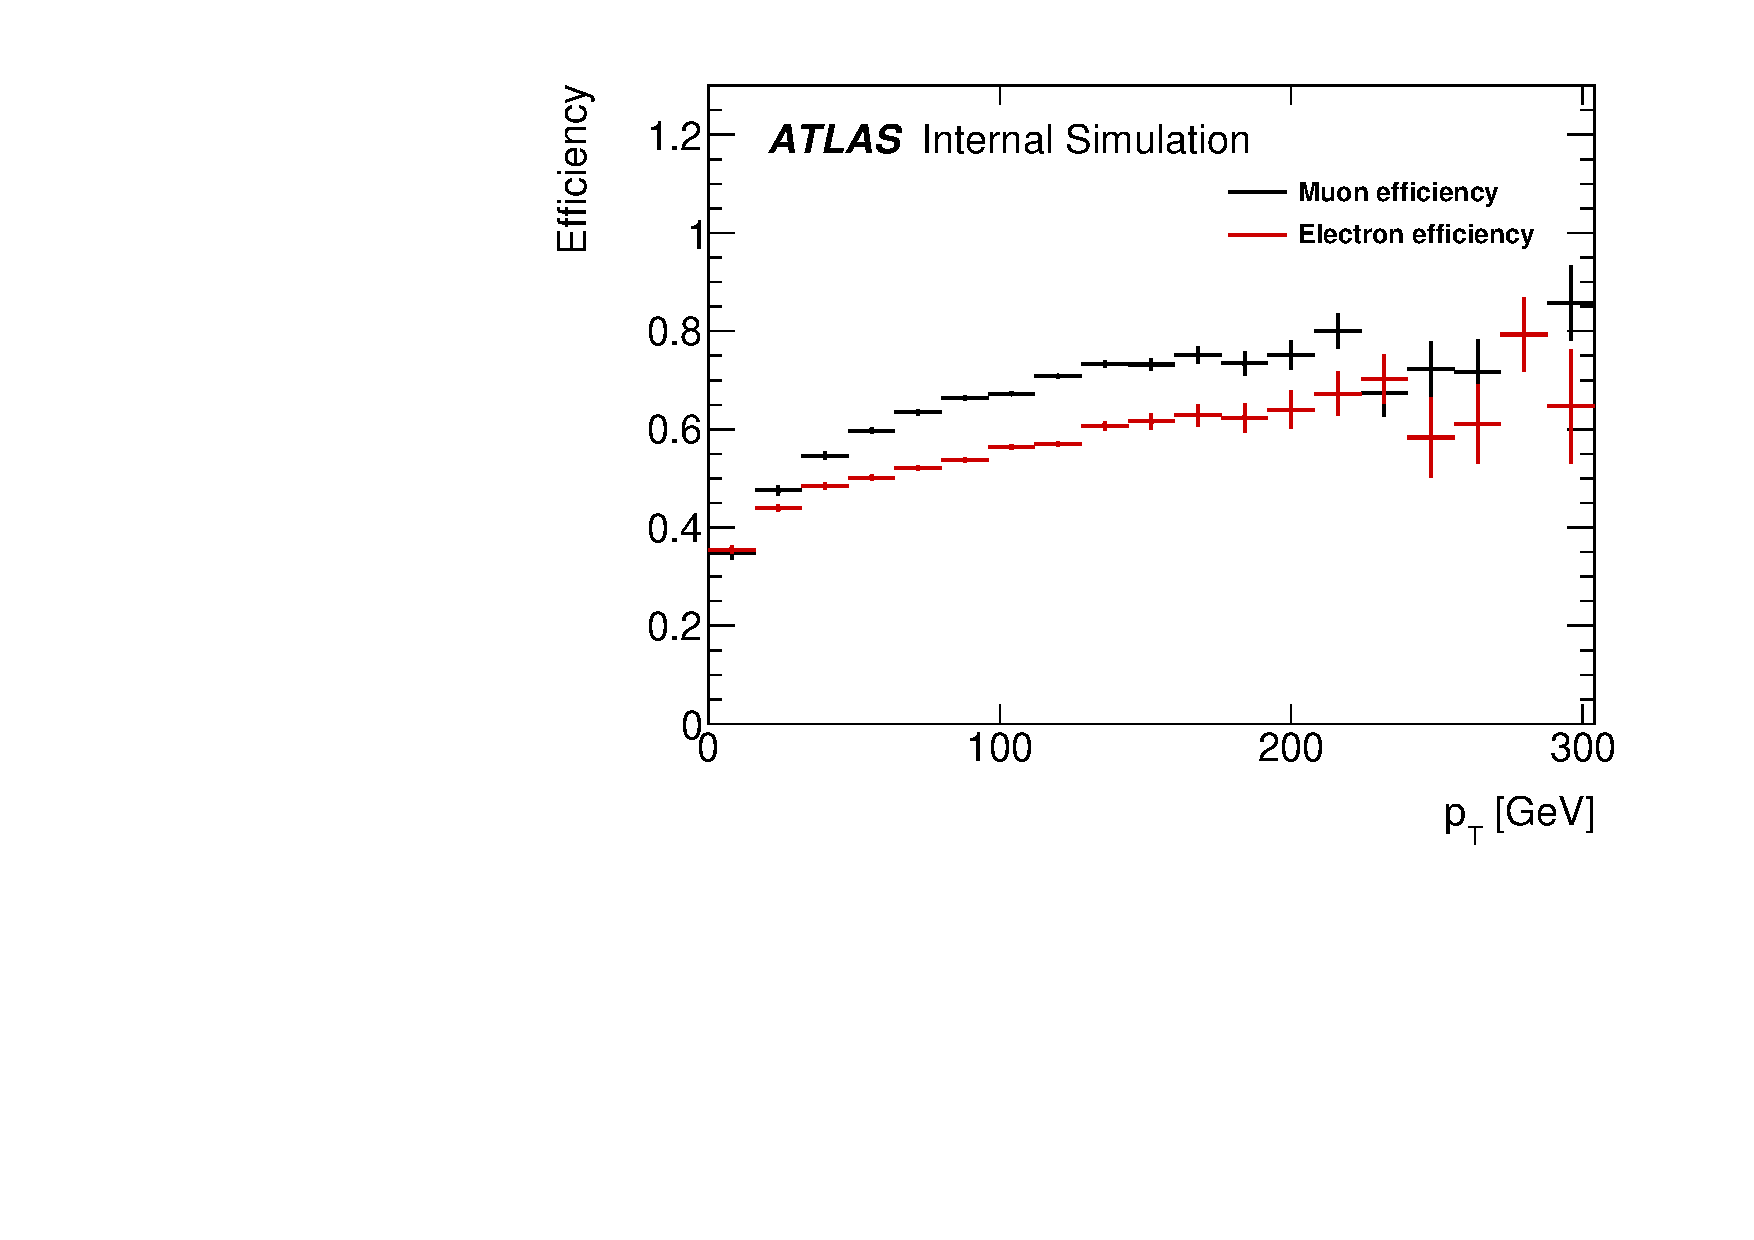
\includegraphics[width=0.50\textwidth]{figures/m_lepton_efficiency_pt.pdf}} 
    \caption{Lepton reconstruction efficiency as a function of (a) $d_{0}$, (b) $z_{0}$, (c) $\eta$, and (d) $p_{T}$ of signal leptons using the signal MC sample generated with $m=$ 250 GeV and $c\tau=$ 250 mm.}
    \label{fig:lepton_eff}
\end{figure}

It is evident that the efficiency drops drastically at $\eta > 2.0$ where the Pixel barrel region ends due to the minimum silicon hits requirement on tracks as shown in Table~\ref{table:lrt_comparison}. The efficiency is not very sensitive to $p_{T}$ except low $p_{T}$ region ($p_{T} < 20$).

The lepton reconstruction efficiency decreases for large $d_{0}$ and $z_{0}$. In the signal MC samples, most of $Z'$ decay within the Pixel barrel region, $r < $ 122.5 mm and $z < $ 400.5 mm, where the lepton reconstruction efficiency is high.

\section{Overall reconstruction efficiency}
\label{sec:combined_reco_efficiency}
The overall reconstruction efficiency is defined as the ratio of $Z'$s reconstructed as displaced vertices in the signal region to the total $Z'$ produced in the sample. In this section, representative plots of event cut flow, vertex cut flow (Section~\ref{sec:signal_cutflow}), and overall reconstruction efficiency distributions (Section~\ref{sec:signal_vertex_distribution}) are presented using the signal MC samples generated with $m=$ 500, 1000 GeV, and $c\tau=$ 100 mm.
%to provide a model-independent result that matches well with the data sample.

In Section~\ref{sec:efficiency_reweighting}, the overall reconstruction efficiency is reweighted to reproduce pile-up distribution in the data sample. The reconstruction efficiency for all MC samples is also presented.


\subsection{Event and vertex cut flow}
\label{sec:signal_cutflow}
The MC samples are processed with steps described in Section~\ref{sec:preselection}. The analysis level cuts, the event and the vertex selections described in Table~\ref{table:signal_selection}, are applied to the processed samples. Representative plots of the event cut flow and the vertex cut flow are shown in Figure~\ref{fig:signal_cutflow_MC_mumu} using the signal MC samples of $Z'$ decaying to $\mu\mu$ generated with $m=$ 500, 1000 GeV for $c\tau=$ 100 mm.

\begin{figure}[!htb]
    \centering
    \subfloat[]{\label{subfig:event_cutflow_MC}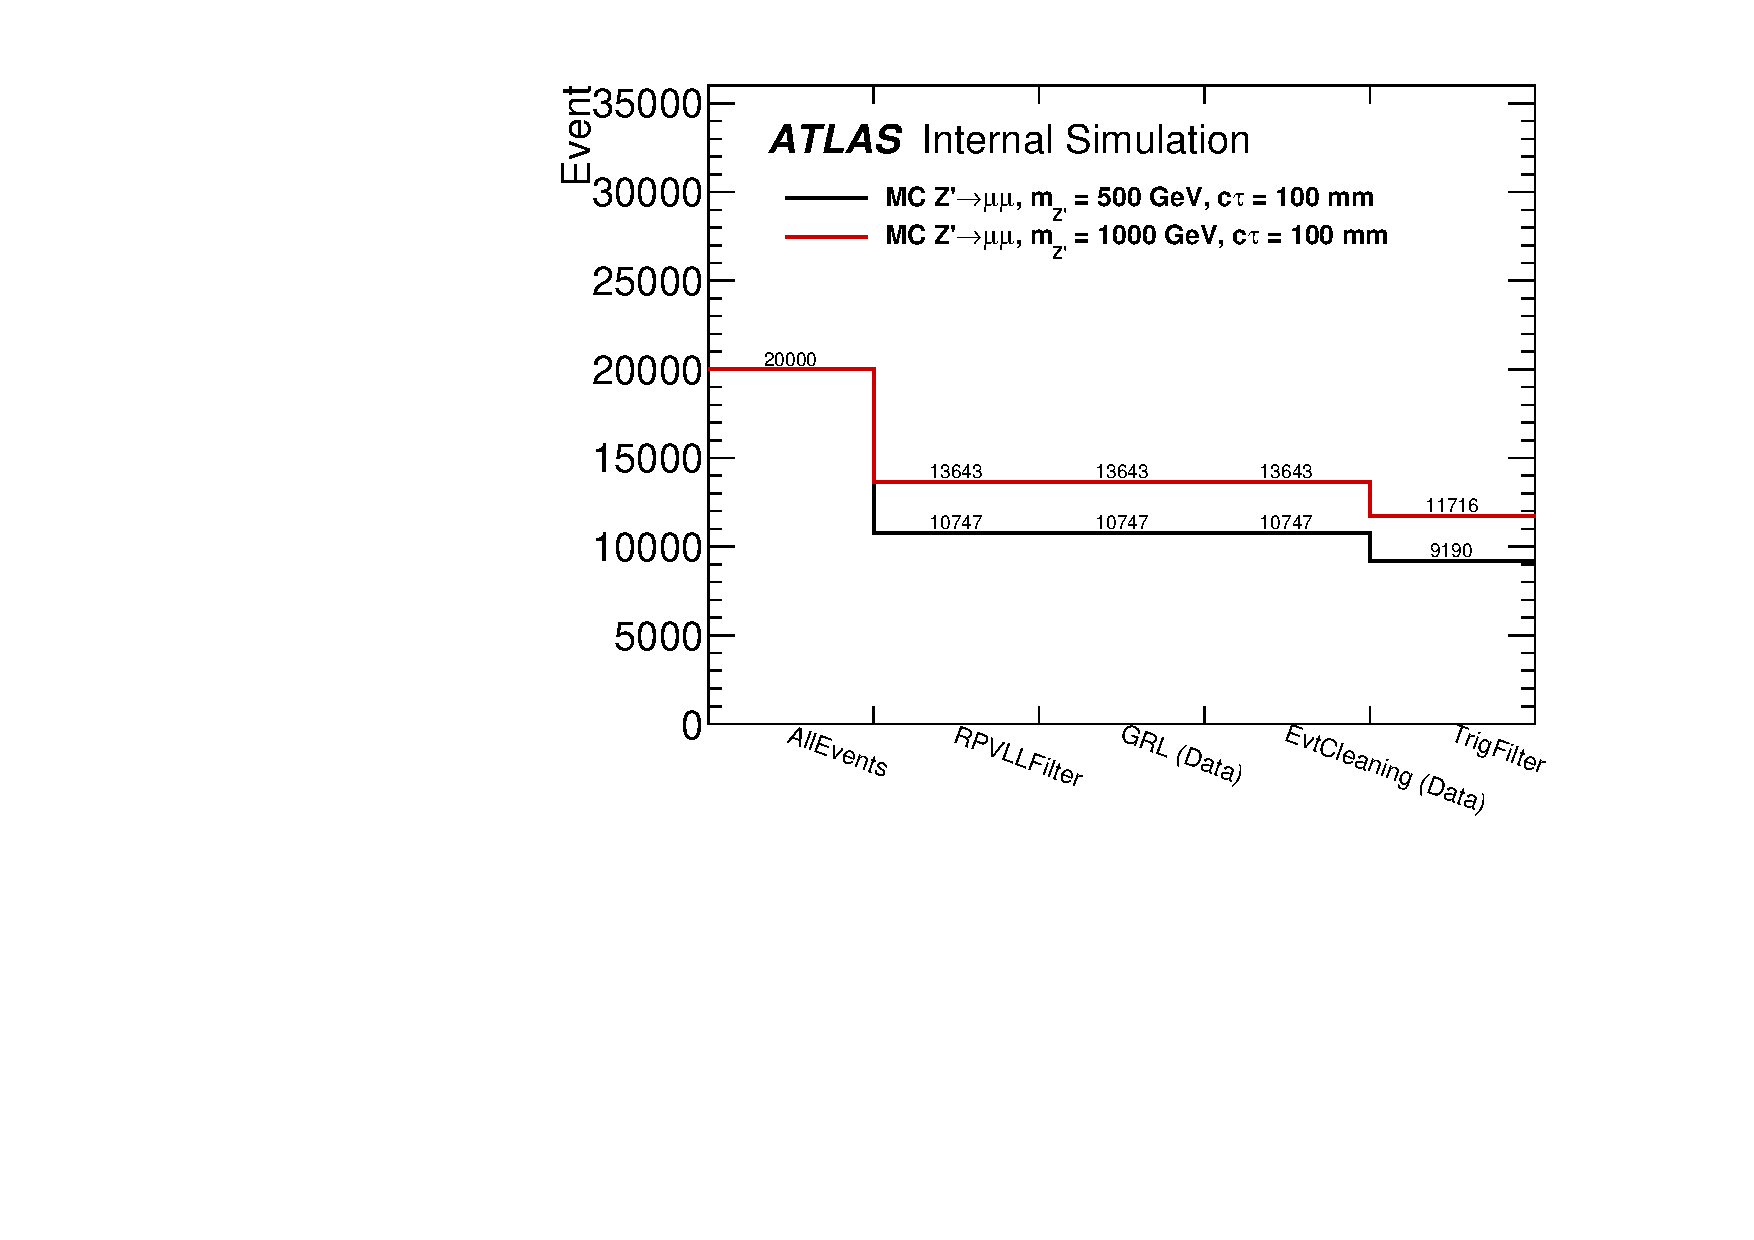
\includegraphics[width=0.50\textwidth]{figures/m_event_cutflow_MC_mumu.pdf}}
    \subfloat[] {\label{subfig:vertex_cutflow_MC}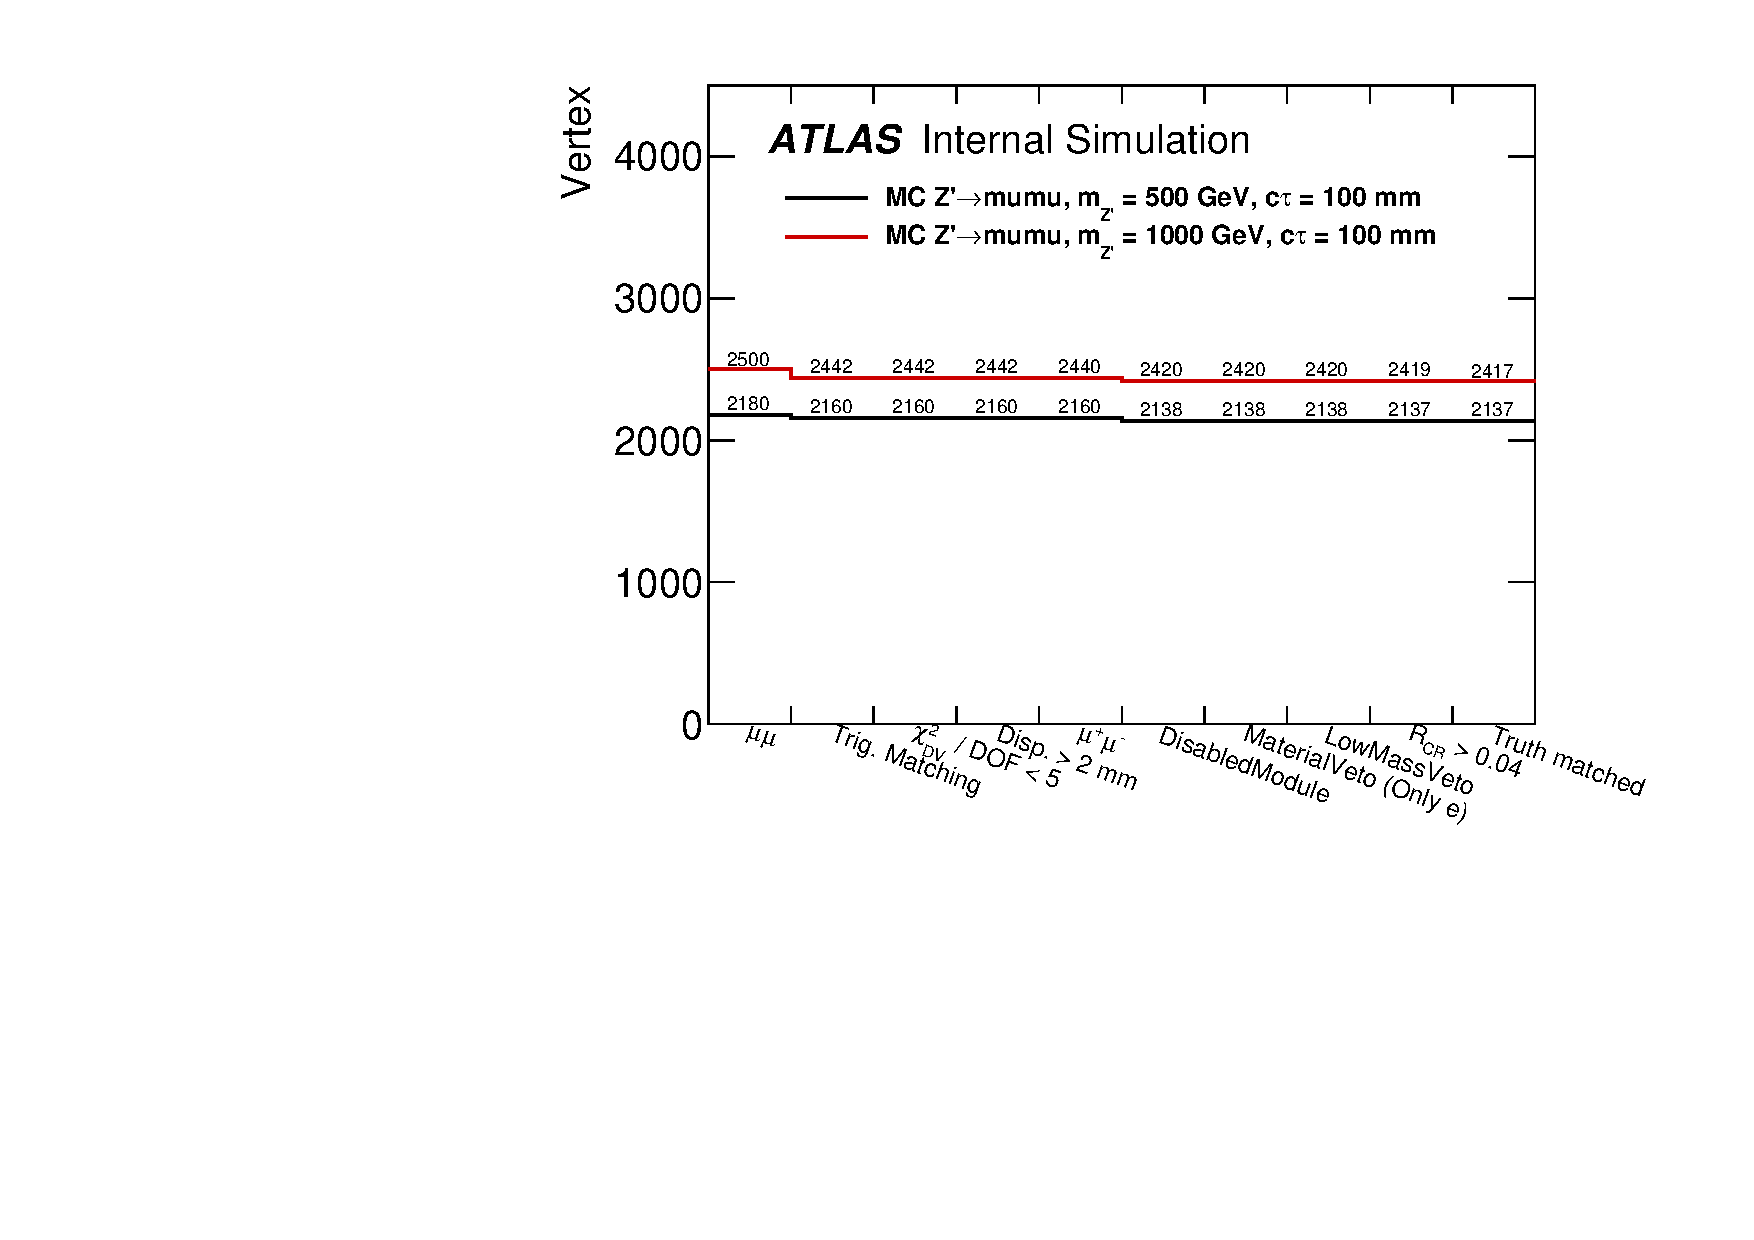
\includegraphics[width=0.50\textwidth]{figures/m_dv_cutflow_MC_mumu.pdf}} \\
    \caption{(a) Event cut flow, and (b) vertex cut flow using the signal MC samples of $Z'\rightarrow \mu\mu$ generated with $m =$ 500,1000 GeV for $c\tau= $ 100 mm.}
    \label{fig:signal_cutflow_MC_mumu}
\end{figure}

In the event cut flow, \texttt{RPVLL} filter is applied during the sample processing. \texttt{GoodRunsList} filter and Event cleaning are shown as place holders as they are only applied to data sample.

In the vertex cut flow, displaced vertices are reconstructed in about $\backsim$25$\%$ of the signal events passing the event selection, indicating that there is a significant loss of signal efficiency in the reconstruction process. The following selection criteria, $\chi^{2} /$ DOF $<$ 5 and the minimum displacement cut ($r > $ 2 mm), are applied, but the effect is expected to be very small as the same requirements are applied in the secondary vertex reconstruction algorithm. Material veto is applied to all vertex types except $\mu\mu$ vertex. The minimum dilepton mass requirement and cosmic veto cuts have minimum impact on the signal efficiency.

\subsection{Efficiency distribution}
\label{sec:signal_vertex_distribution}
The overall reconstruction efficiency is studied by examining the efficiency distributions in the transverse ($r$), longitudinal ($z$) vertex position, and the angular distributions of the reconstructed vertices. The representative efficiency distributions are shown in Figure~\ref{fig:signal_vertex_dist} using the signal MC samples generated with $m =$500, 1000 GeV for $c\tau=$100 mm.

The overall efficiency shows a significant dependence on vertex position which decreases at large $r$ and $z$ due to the minimum silicon hits requirement on tracks. The first bins in $r$ and $z$ distributions have lower efficiency due to the minimum displacement requirement ($r > $ 2 mm) on secondary vertices. The $r$ distribution shows features that reflects the physical structure of the ID. The $\eta$ distribution has higher efficiency in the central region, and the $\phi$ distribution is uniform as expected.


\begin{figure}[!htb]
    \centering
    \subfloat[]{\label{subfig:vertex_dist_r  }\includegraphics[width=0.50\textwidth]{figures/m_dv_efficiency_r.pdf}}
    \subfloat[]{\label{subfig:vertex_dist_z  }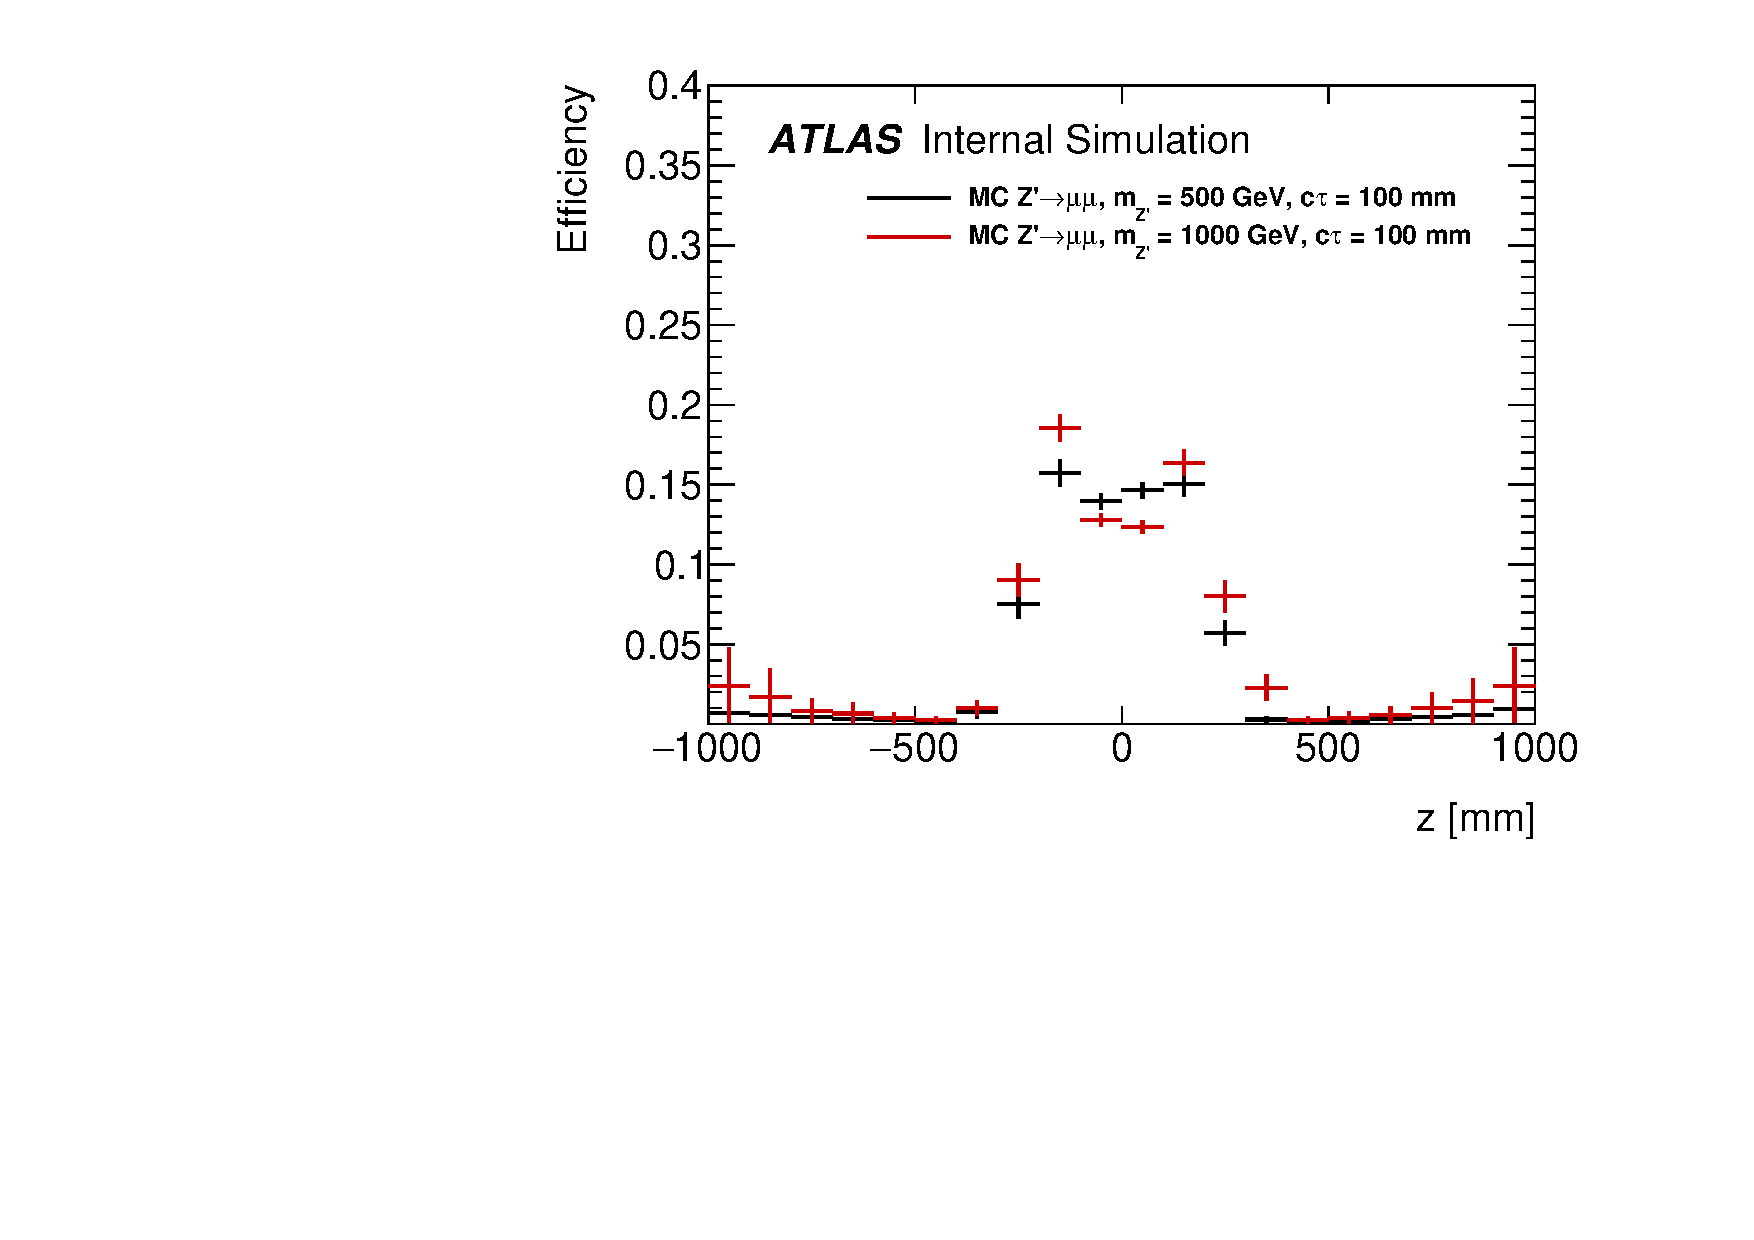
\includegraphics[width=0.50\textwidth]{figures/m_dv_efficiency_z.pdf}} \\
    \subfloat[]{\label{subfig:vertex_dist_eta}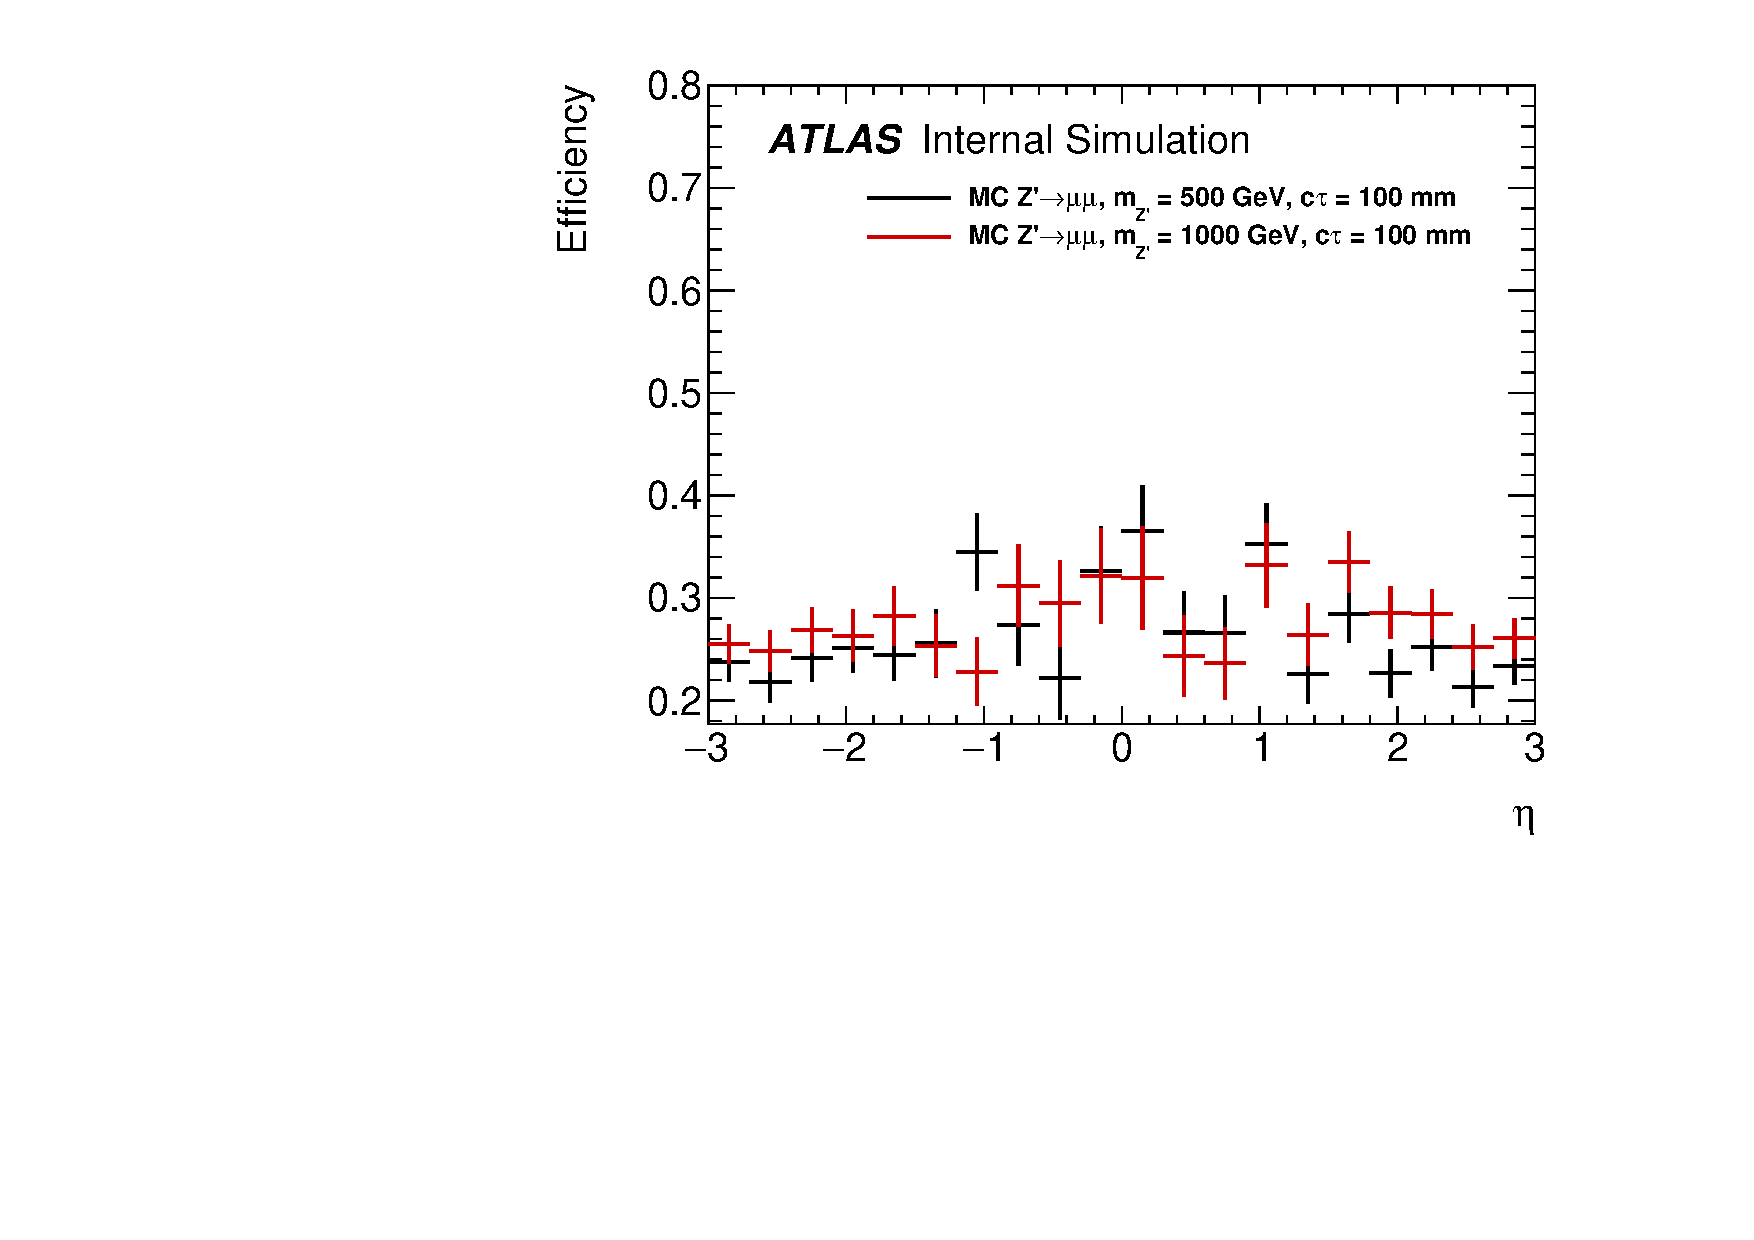
\includegraphics[width=0.50\textwidth]{figures/m_dv_efficiency_eta.pdf}}
    \subfloat[]{\label{subfig:vertex_dist_phi}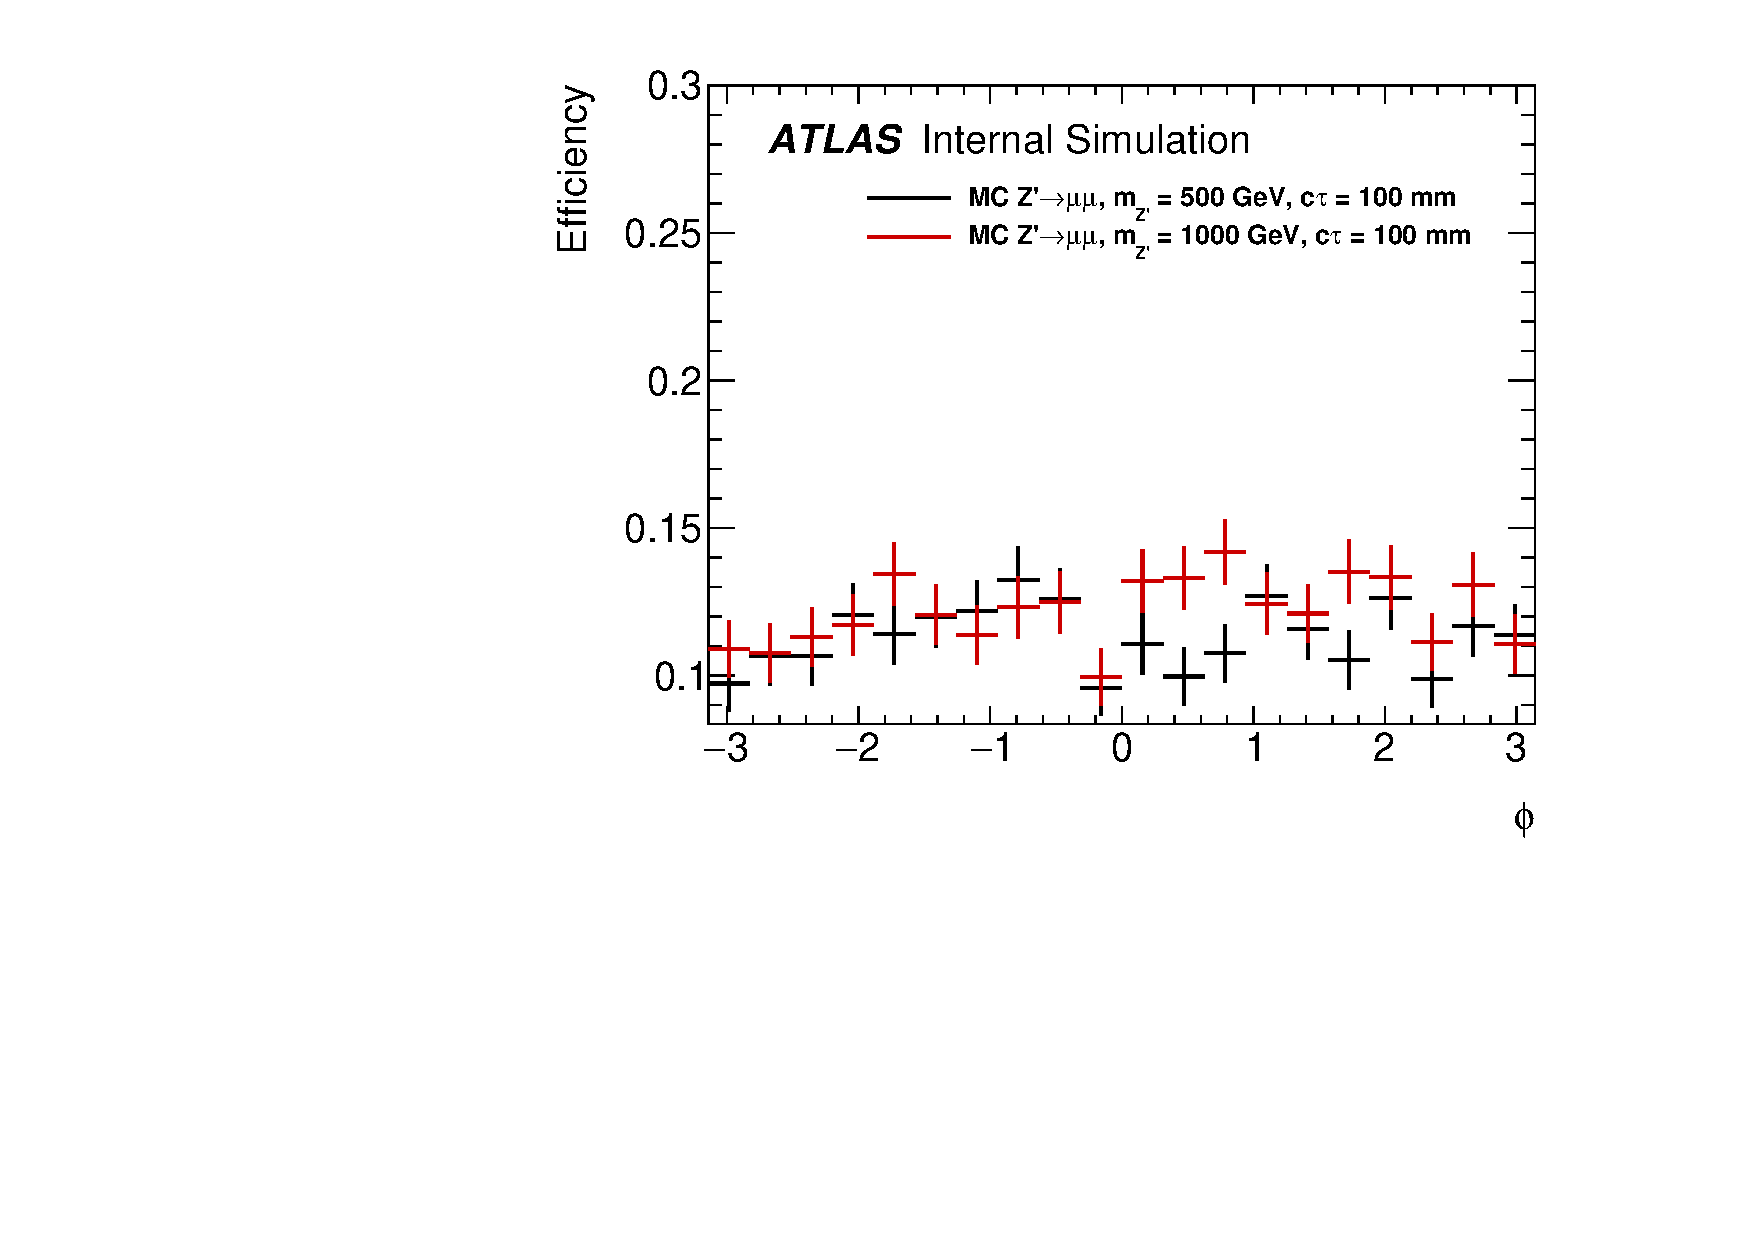
\includegraphics[width=0.50\textwidth]{figures/m_dv_efficiency_phi.pdf}} 
    \caption{The overall efficiency distributions in (a) $r$, (b) $z$, (c) $\eta$, and (d) $\phi$ of the signal MC samples of $Z'\rightarrow \mu\mu$ with $m=$ 500, 100 GeV for $c\tau=$ 100 mm.}
    \label{fig:signal_vertex_dist}
\end{figure}

\subsection{Efficiency reweighting}
\label{sec:efficiency_reweighting}




%\begin{table}[!htb]
%  \centering
%  \begin{tabular}{ c c | c c  }
%    \hline
%           &       & \multicolumn{2}{c}{$Z'\rightarrow\mu\mu$}                \\
%    $m_{Z'}$ (GeV) & $c\tau$ (mm) & unweighted & reweighted \\
%    \hline
%    100			&	100	& 0.0472$\pm$0.0026 	&0.0593$\pm$0.0033  \\
%    100			&	250	& 0.0323$\pm$0.0021 	&0.0399$\pm$0.0028 	\\
%    100			&	500	& 0.0184$\pm$0.0016		&0.0243$\pm$0.0023 	\\
%    250			&	100	& 0.2010$\pm$0.0049		&0.2200$\pm$0.0058	\\
%    250			&	250	& 0.1759$\pm$0.0046 	&0.1848$\pm$0.0053	\\
%    250			&	500	& 0.1315$\pm$0.0042		&0.1375$\pm$0.0048	\\
%    500			&	100	& 0.2284$\pm$0.0053		&0.2473$\pm$0.0062	\\
%    500			&	250	& 0.2001$\pm$0.0049		&0.2083$\pm$0.0056	\\
%    500			&	500	& 0.1554$\pm$0.0045 	&0.1629$\pm$0.0052 	\\
%    750			&	100	& 0.2340$\pm$0.0052		&0.2485$\pm$0.0060 	\\
%    750			&	250	& 0.2277$\pm$0.0051		&0.2341$\pm$0.0058 	\\
%    750			&	500	& 0.1654$\pm$0.0045		&0.1670$\pm$0.0050  \\
%    1000	    &	100	& 0.2253$\pm$0.0051 	&0.2421$\pm$0.0059 	\\
%    1000	    &	250	& 0.2301$\pm$0.0050 	&0.2337$\pm$0.0057	\\
%    1000	    &	500	& 0.1871$\pm$0.0047  	&0.1854$\pm$0.0052  \\
%    \hline
%  \end{tabular}
%  \caption{}
%  \label{table:m_signal_eff_mumu_all}
%\end{table}





%TABLE SHOWING ALL EFFICIENCY GOES HERE


%-------------------------------------------------------------------------------
\section{Background estimation}
\label{sec:background_estimation}
Due to the lifetime ($c\tau > 2$ mm) and mass ($m > 10$ GeV) requirements applied at vertex selection, no SM background is expected in the signal region in search for displaced dilepton resonance. Therefore, two non-collision backgrounds and background from low-mass vertices are considered in this search. In Section~\ref{sec:random_crossing}, background from \textit{random-crossing} of two uncorrelated tracks are estimated. The cosmic ray background is estimated in Section~\ref{sec:cosmic_ray}, and the low-mass background which results from low-mass vertices is estimated in Section~\ref{sec:low_mass}

\subsection{Random-crossing background}
\label{sec:random_crossing}
%High luminosity in 2016 data ($\langle\mu\rangle\approx 24.9$) %where $<\mu>$ is average number of interactions per bunch crossing, made 
%The random-crossing of two uncorrelated tracks is one of the dominant source of background in search for displaced dilepton vertices due to increasing pileup in Run 2 with $\langle\mu\rangle\approx 24.9$ in 2016 data. 
The random-crossing of two uncorrelated tracks is a major source of the backgrounds in the search for displaced dilepton vertices. This background is expected to increase with more pile up in Run 2.

This random-crossing background is estimated by the \textit{track flipping} method in which secondary vertex reconstruction is performed on each pair of tracks from all possible combinations of tracks after one random track from each pair is flipped with respect to the primary vertex. Because one track is flipped in each pair of tracks, the resulting vertices provide good estimation for random-crossing background.

The track flipping method is tested on the background MC samples. As an additional check, the vertices found from this method are compared with vertices found from another random-crossing background estimation method, the \textit{event mixing}. In Section~\ref{sec:random_crossing_data}, the random-crossing background are estimated using the track flipping method with 32.8 $\mathrm{fb^{-1}}$ of 2016 data sample, and its systematic uncertainties are estimated in Section~\ref{sec:random_crossing_systematics}.

\subsubsection{MC study}
\label{sec:random_crossing_MC}
The track flipping method is tested using the background MC sample with 2.4 M events as described in Section~\ref{sec:data_MC}. Events are selected by the same requirement described in Section~\ref{sec:signal_efficiency}. From the selected events, tracks identified as muon, electron, or neither, referred as muon, electron, or non-leptonic track, respectively, are selected with the track criteria (Table~\ref{table:vertex_track_selection_simple}) as in the secondary vertexing algorithm for consistency. Leptons are required to pass the same selection criteria described in Table~\ref{table:lepton_requirement}. Non-leptonic tracks are required to pass the minimal kinematic selection ($p_{T} > 10 GeV, \eta < 2.5$ to match with the kinematic selection for leptons.

Track pairs are created from all possible combination of muon, electron, or non-leptonic tracks which fall into one of the six categories, $\mu\mu$, $ee$, $e\mu$, $e$x, $\mu$x, or xx track pair, where $x$ represents a non-leptonic track. For each pair of tracks, one track is randomly flipped with respect to the beam spot ($d_{0}\rightarrow -d_{0}, z_{0}\rightarrow -z_{0}, \phi\rightarrow\phi-\pi, \theta\rightarrow\pi-\theta$). The flipped track and the other track in the pair are used to estimate the background from uncorrelated tracks.

%Two tracks from each pair after flipping one track become uncorrelated.

The same secondary vertex algorithm used in the reconstruction of data or MC sample is performed on the track pairs with one track flipped to reconstruct secondary vertices. Vertex selection cuts similar to the cuts listed in Table~\ref{table:vertex_track_selection_simple} are applied to the vertices found by the track flipping. The only differences in the vertex cuts are:
\begin{itemize}
\item Trigger matching is only required for $\mu\mu$, $ee$, and $e\mu$ vertices because non-leptonic tracks cannot be matched to lepton triggers, 
\item Filter matching is only required for $\mu\mu$, $ee$, and $e\mu$ vertices for the same reason.
\end{itemize}

Because trigger and filter matchings are not required in the control and validation region, the track flipping method provides conservative background estimation. Figure~\ref{fig:m_FBE_cutflow_MC} shows the vertex cut flow applied on xx vertices from the background MC samples.

%\begin{figure}[!htb]
\begin{figure}[tb]
	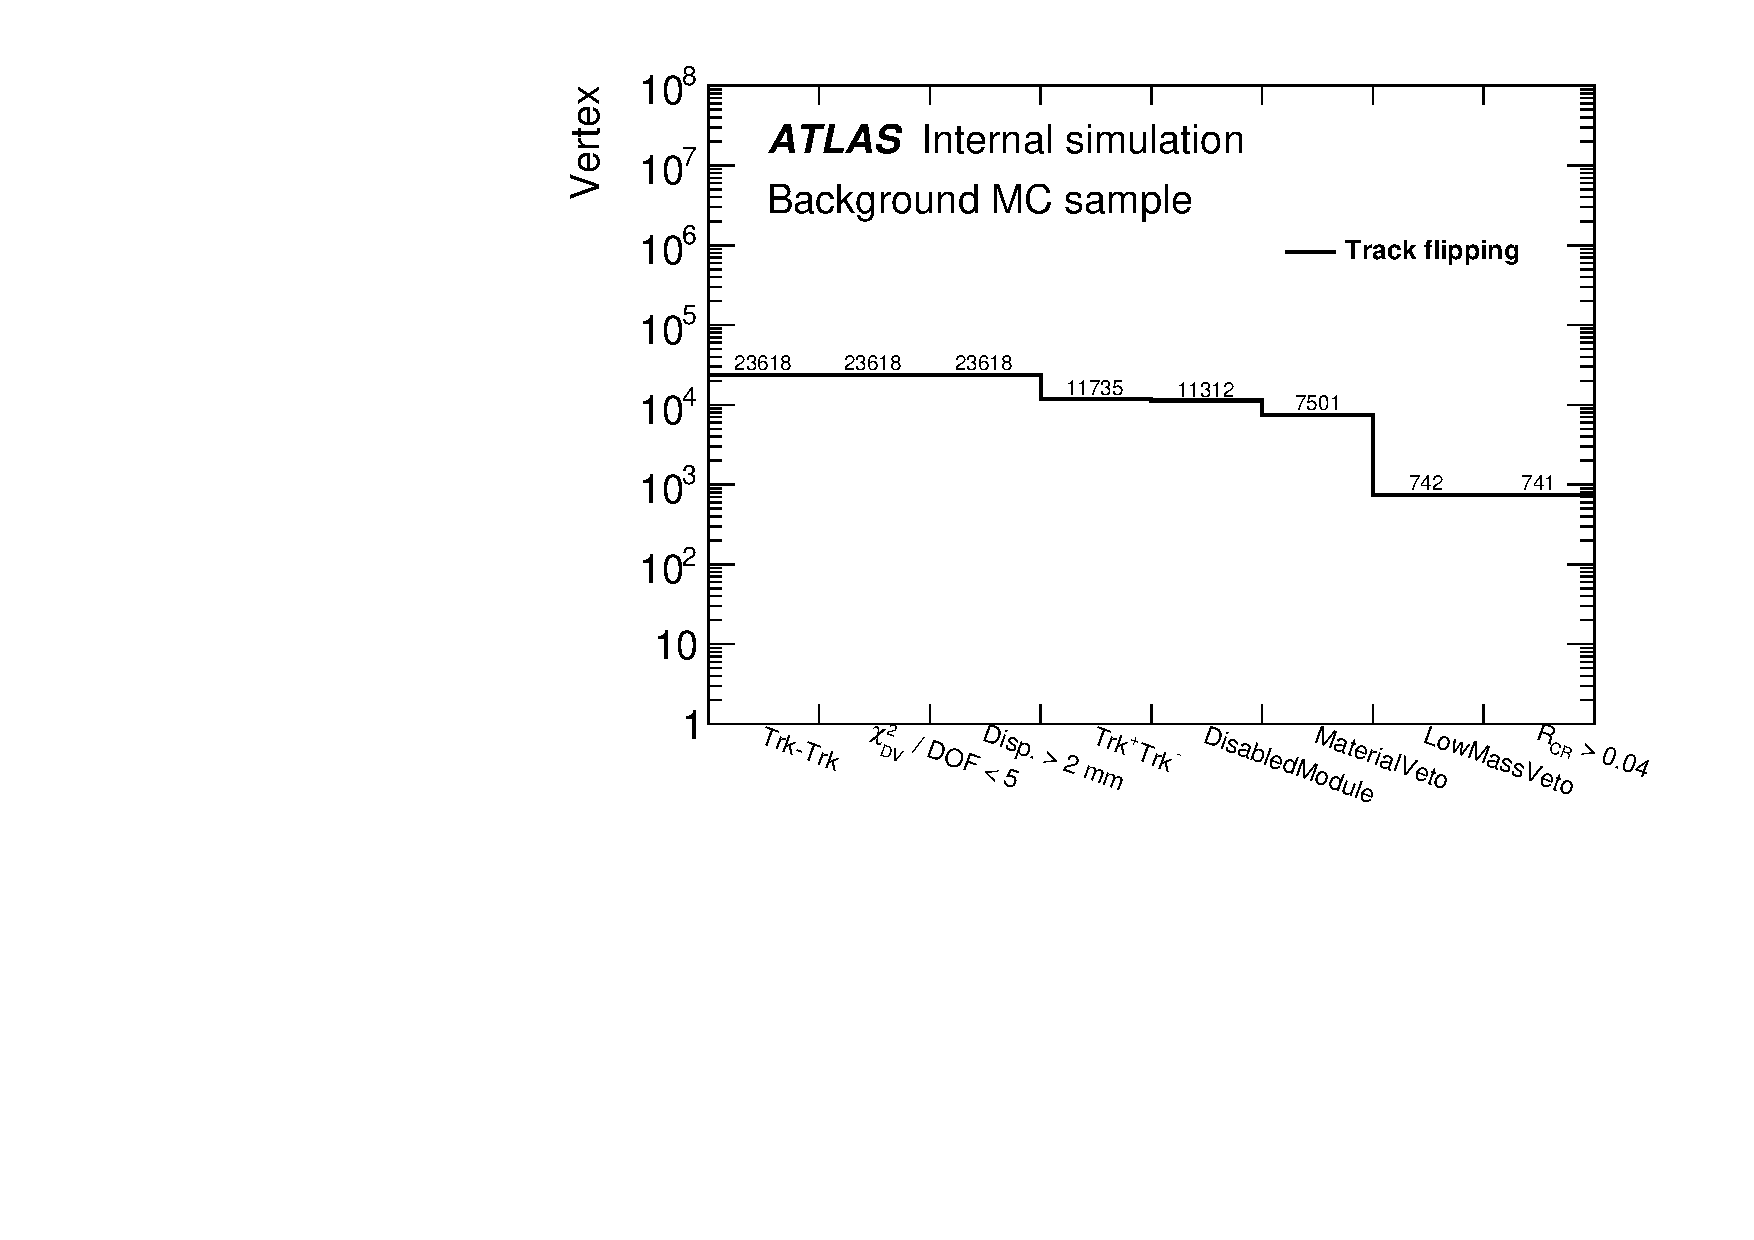
\includegraphics[width=0.60\textwidth]{figures/m_FBE_cutflow_MC.pdf}
	\centering
	\caption{Vertex cut flow applied on xx vertices from the track flipping method}
	\label{fig:m_FBE_cutflow_MC}
\end{figure}

The resulting vertices, referred as track-flipping vertices, are compared with the vertices reconstructed by the reconstruction described in Section~\ref{sec:track_vertex_reconstruction} in the MC samples. The same event selection and the vertex selection described in Section~\ref{sec:signal_efficiency} are applied to the vertices in the data sample. Because of minimum invariant mass ($m > 10$ GeV), minimum displacement ($r_{DV} > 2$ mm), and cosmic veto ($R_{\mathrm{CR}} > 0.01$) cuts, the reconstructed vertices in the MC sample are expected to be purely from random-crossing.

In addition, the track-flipping are compared with another random-crossing background estimation method, the \textit{event mixing}. In this method, tracks are sampled from data or MC sample, and the probability, denoted by $p_{\mathrm{rc}}$, for a pair of tracks to form a vertex by random-crossing is estimated by randomly mixing tracks from different events. Using $p_{\mathrm{rc}}$ and the total number of pairs of tracks in data or MC sample, random-crossing background is estimated. The details on this method can be found in []. The same event, track, and vertex selections are applied for consistency with the track flipping.

The xx vertices found from the track flipping, reconstructed in the MC sample, and the estimation from the \textit{event mixing} are compared in Table~\ref{table:random_vertex_count}. No $\mu\mu$, $ee$, or $e\mu$ vertices was found or expected from these methods.
 
\begin{table}[!htb]
  \centering
  \begin{tabular}{ c  c c c }
    \hline
    \hline
	Vertex Type					&Track flipping	&\textit{Event Mixing}	& Background MC Samples \\
    \hline
	$\mu$x						&	1						&	1.3 				&	0					\\
	$e$x						&	0						&	0.3 				&	0					\\
	xx						&	741 					&	714.0				&	676 				\\
    \hline
    \hline
  \end{tabular}
  \caption{Comparison of the number of xx vertices found in the track flipping, estimated from the \textit{event mixing}, and reconstructed in the background MC samples.}
  \label{table:random_vertex_count}
\end{table}

The xx vertex yields from the track flipping and the \textit{event mixing} methods agree within the statistical uncertainty. The xx vertex distributions of the vertices from the track flipping, \textit{event mixing}, and from reconstruction are shown in Figure~\ref{fig:random-crossing_vertex_dist}. The distributions of the track flipping and the \textit{event mixing} agree reasonably well with the distributions of vertices found from the reconstruction.

%, and both methods slightly over-estimated the random-crossing background by $\approx 5.8\%$ in the case of xx vertices.

\begin{figure}[!htb]
    \centering
    \subfloat[]{\label{subfig:random-crossing_M}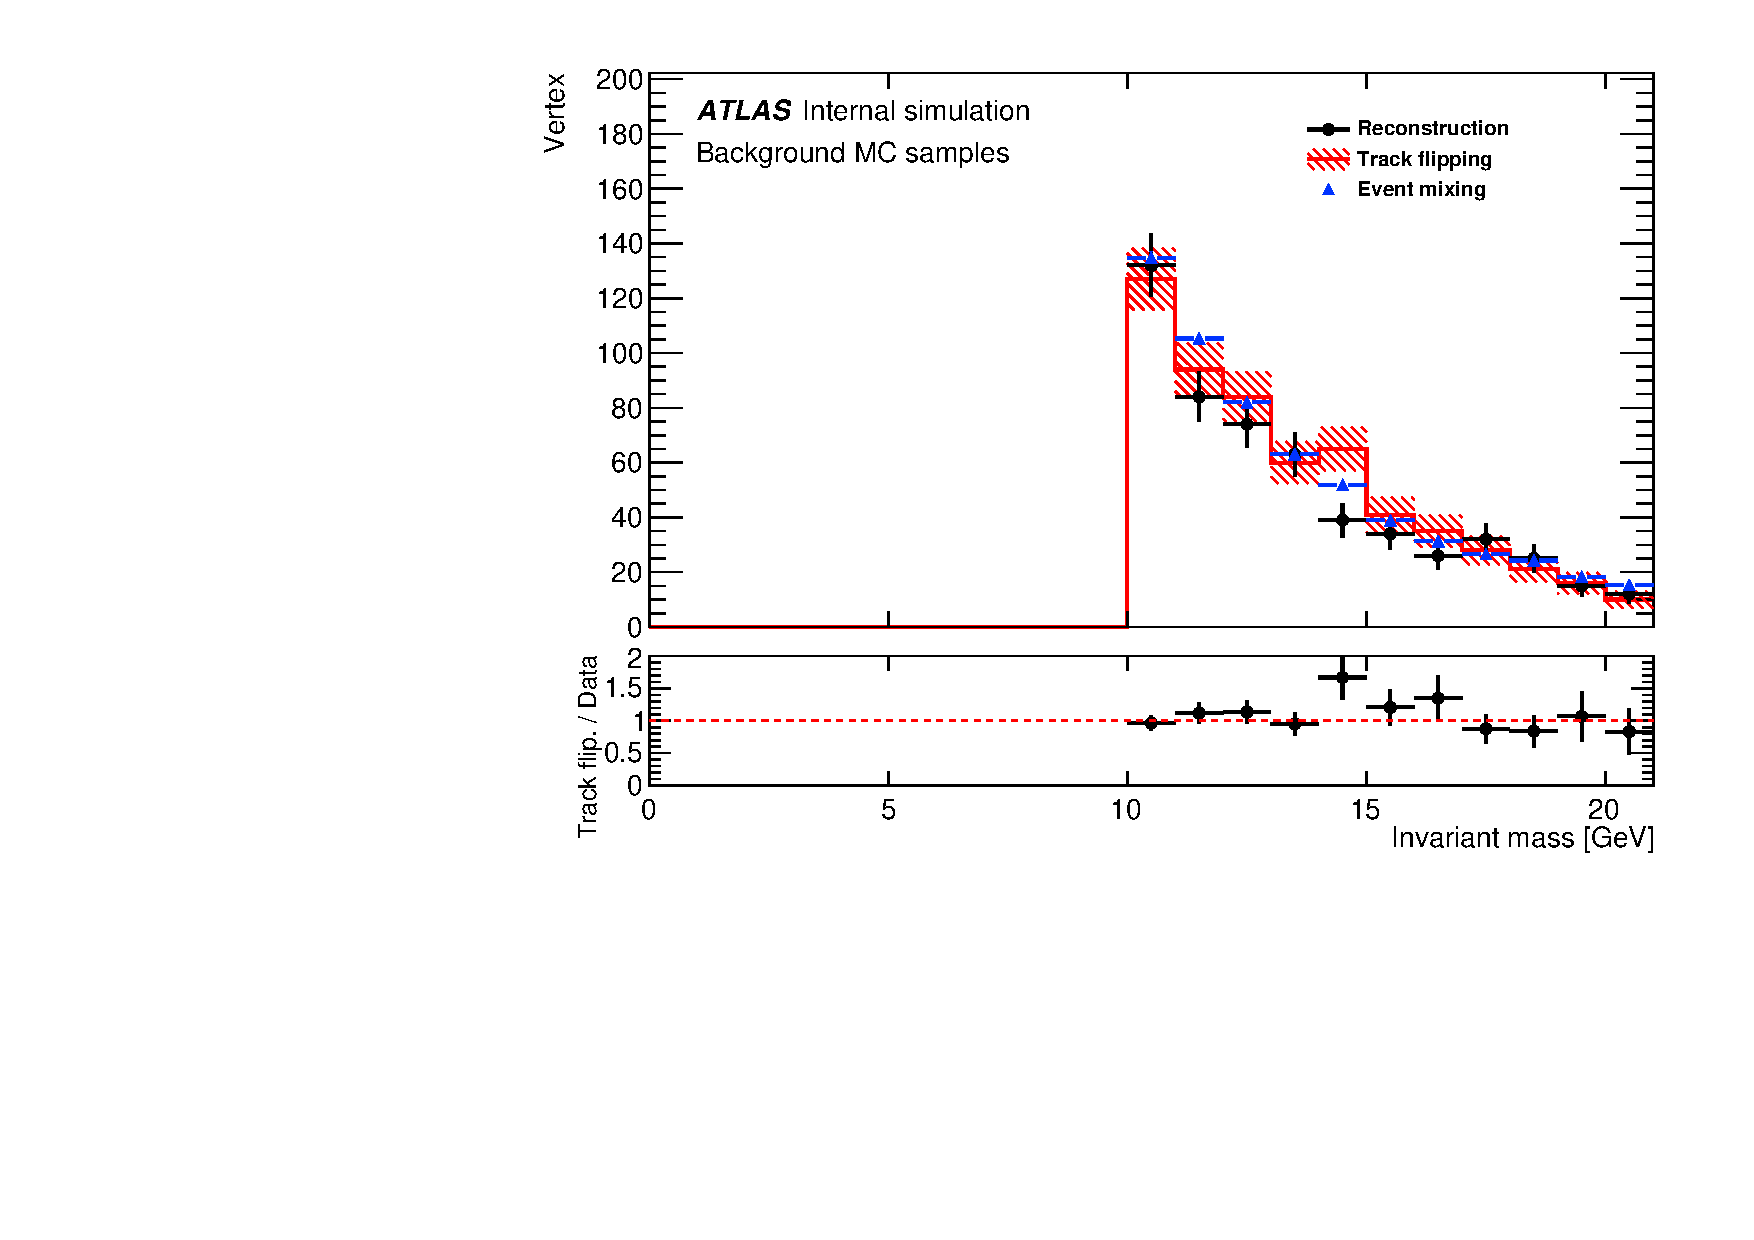
\includegraphics[width=0.45\textwidth]{figures/m_FBE_M.pdf}}
    \subfloat[]{\label{subfig:random-crossing_chi2ndof}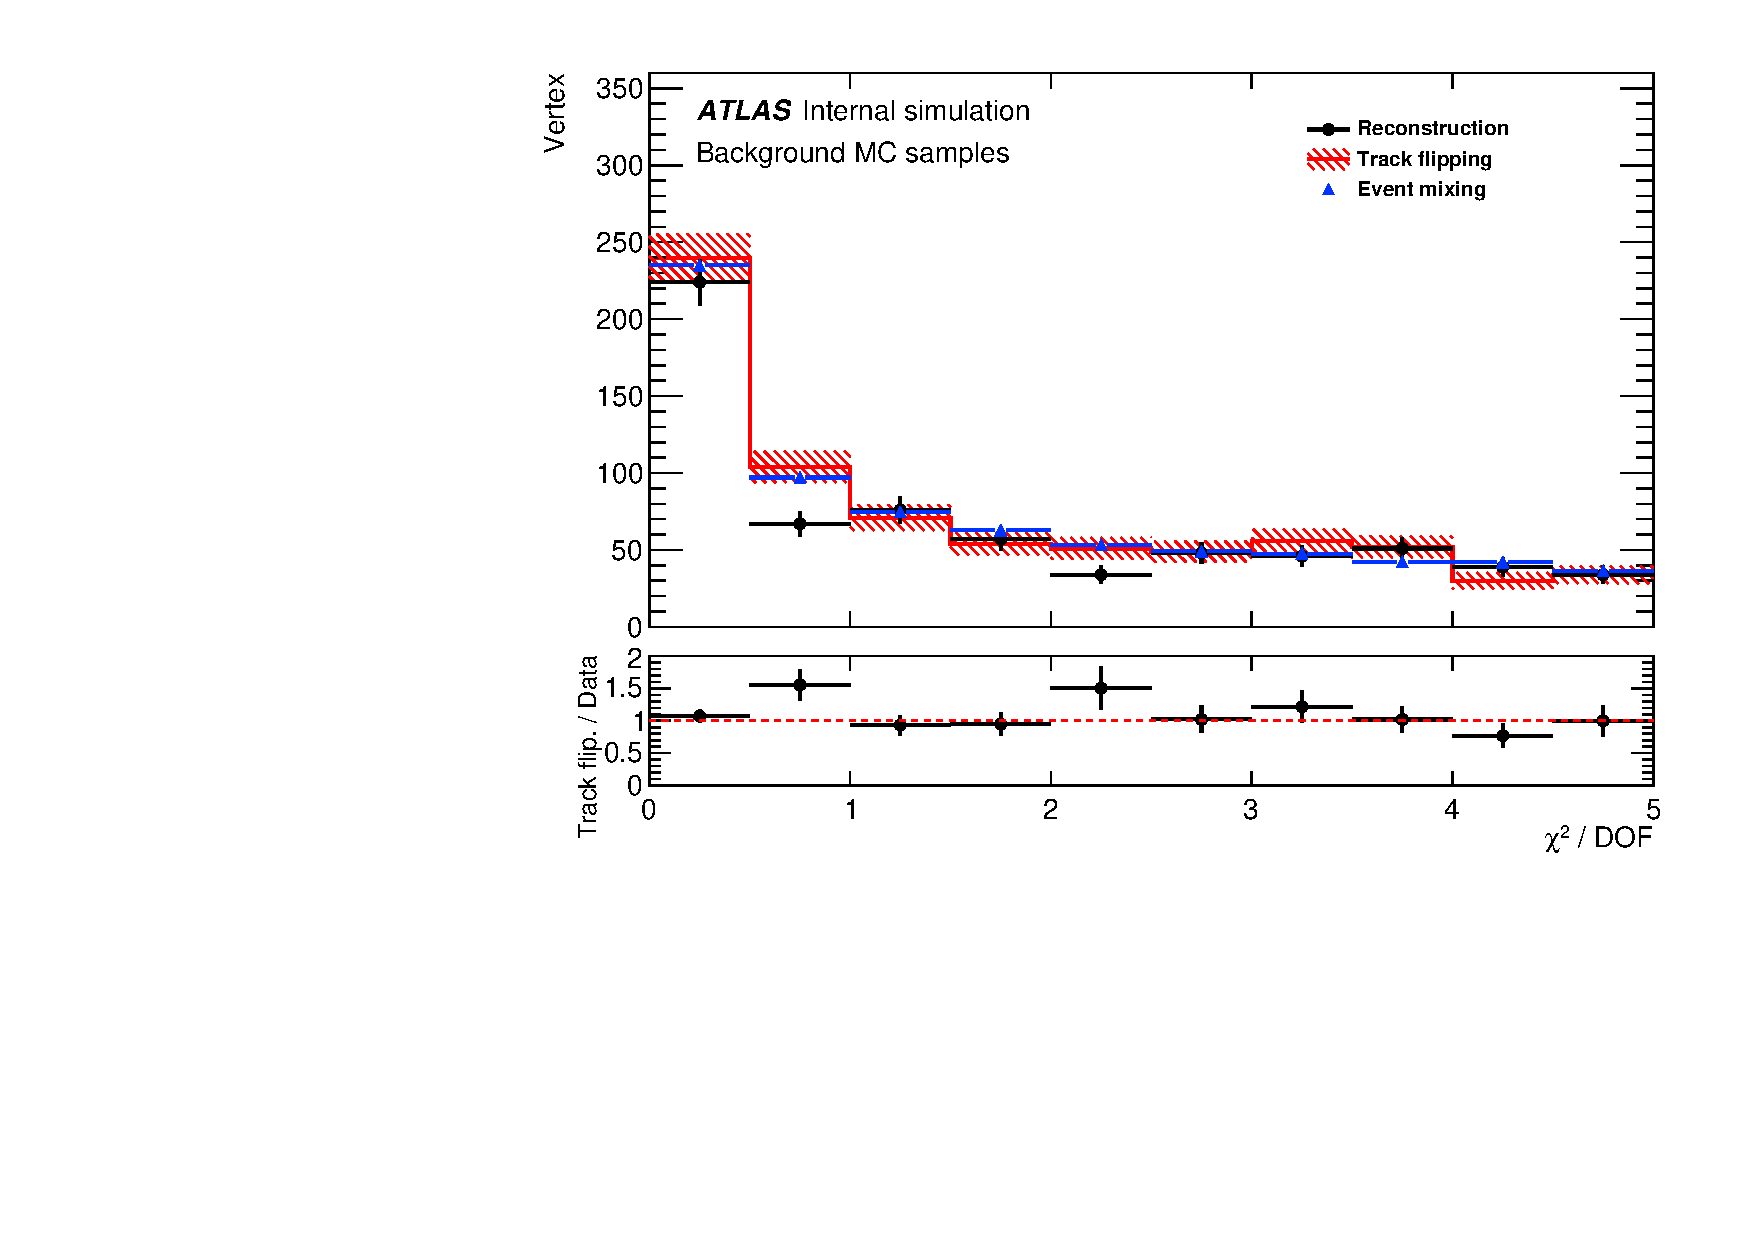
\includegraphics[width=0.45\textwidth]{figures/m_FBE_chi2_ndof.pdf}} \\
    \subfloat[]{\label{subfig:random-crossing_r}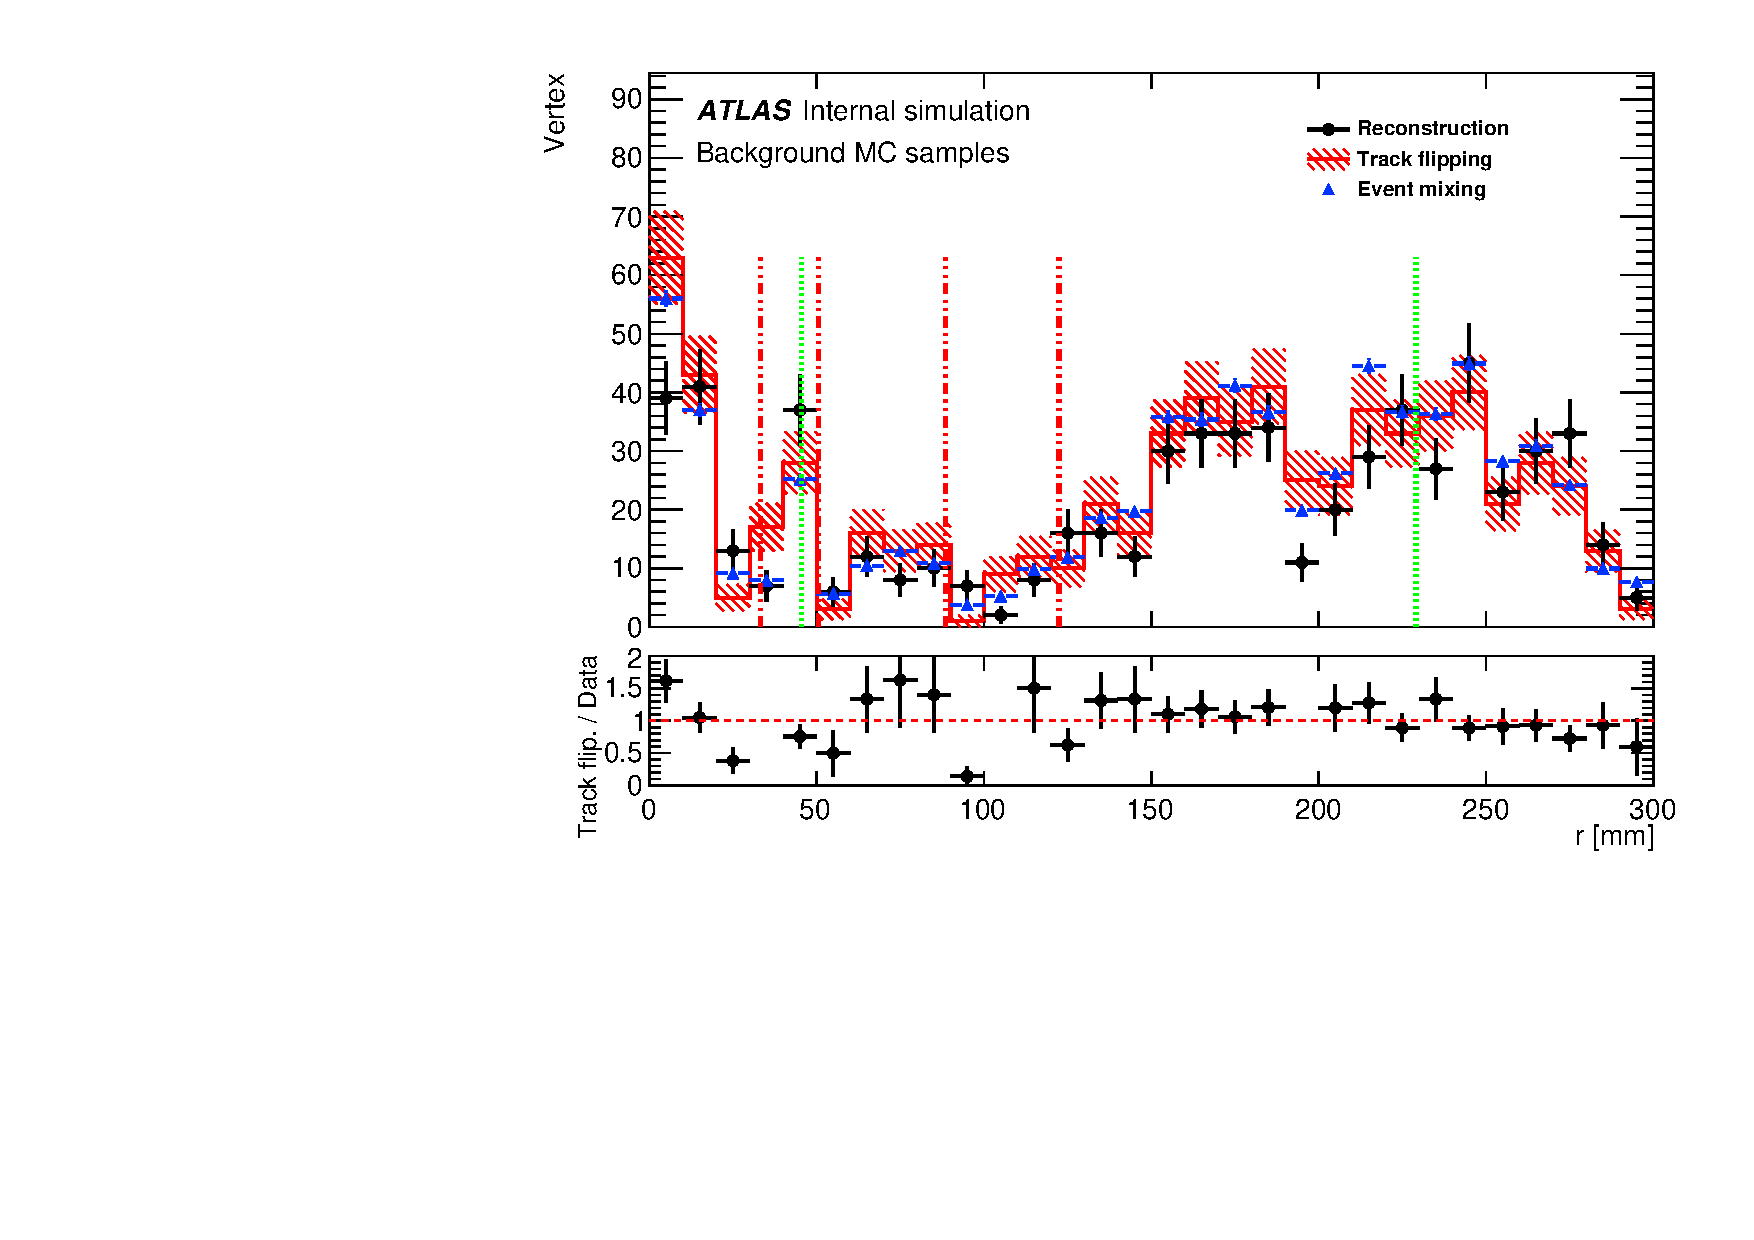
\includegraphics[width=0.45\textwidth]{figures/m_FBE_R.pdf}}
    \subfloat[]{\label{subfig:random-crossing_z}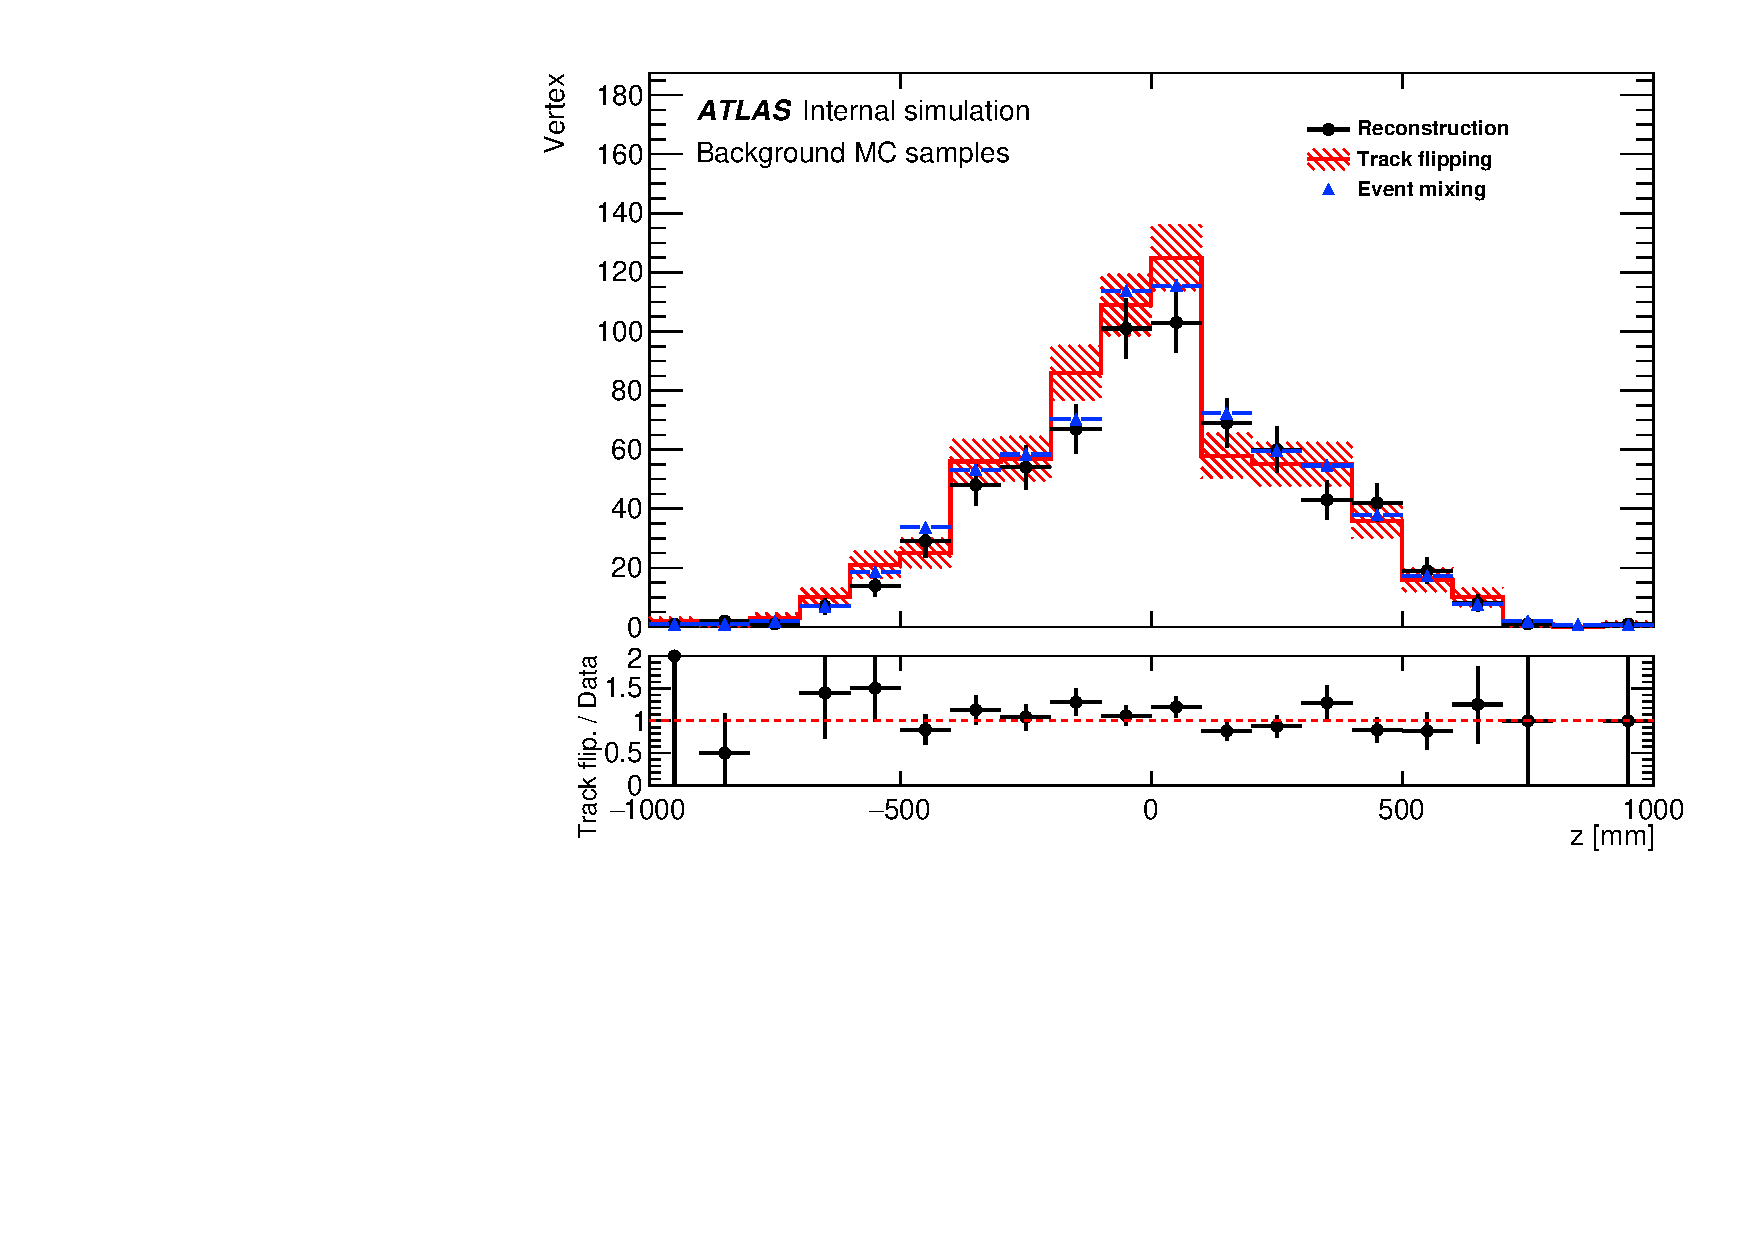
\includegraphics[width=0.45\textwidth]{figures/m_FBE_z.pdf}}
    %\subfloat[l]{\label{subfig:random-crossing_l}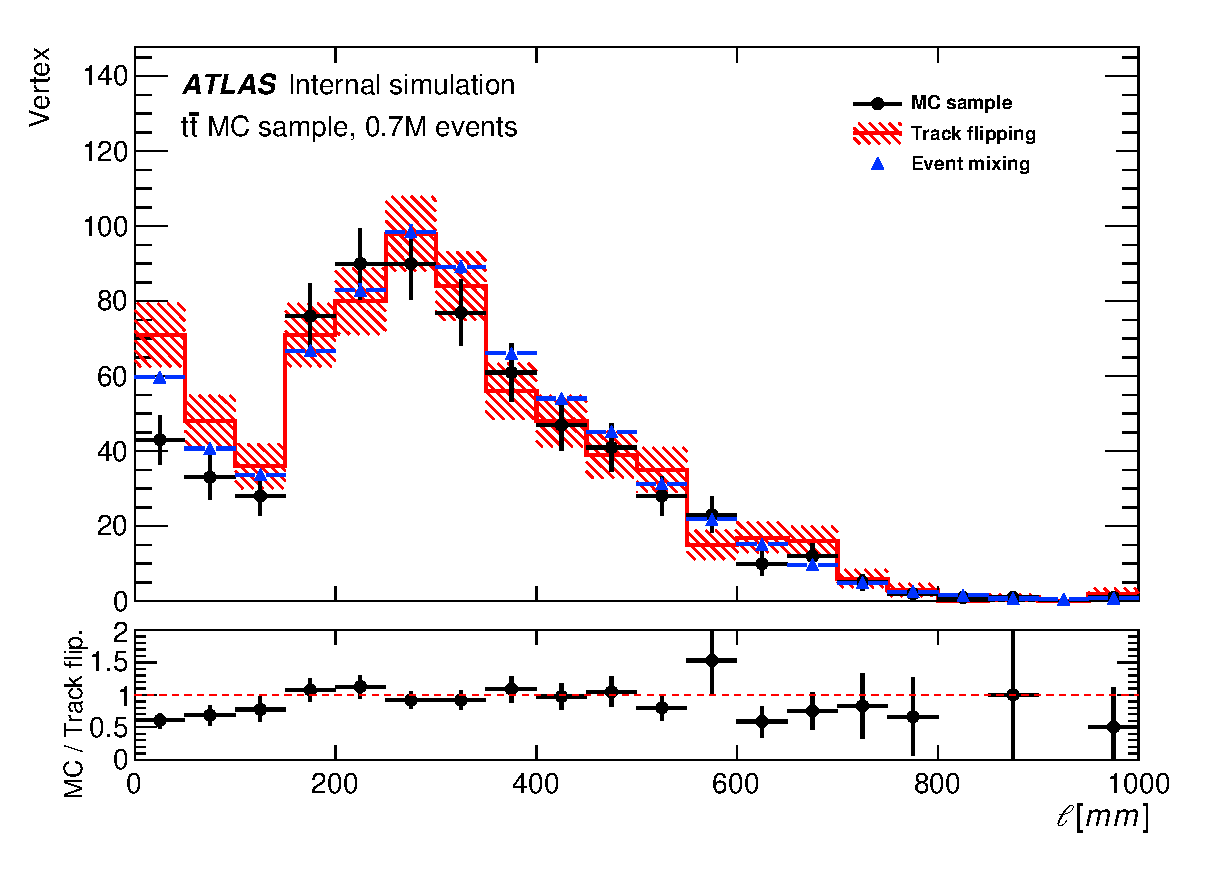
\includegraphics[width=0.45\textwidth]{figures/m_FBE_l.eps}}
    \caption{Comparison of of (a) vertex mass, (b) $\chi^{2} / \mathrm{DOF}$, (c) transverse, and (d) longitudinal position of xx vertices reconstructed, found from the track flipping, and estimated using the \textit{event mixing}. In (c), the red dashed lines indicate the four Pixel layers and the first layer of SCT. The green dotted lines indicate the Inner Support Tube (45.5 mm) and Pixel Support Tube (229 mm).}
    \label{fig:random-crossing_vertex_dist}
\end{figure}

\subsubsection{Estimating random-crossing background with data sample}
\label{sec:random_crossing_data}
Random-crossing background is estimated using 32.8 $\mathrm{fb^{-1}}$ of 2016 data sample described in Section~\ref{sec:data_MC}.

\textbf{Vertex distribution} In control region, the $xx$ vertices found from the track flipping method are compared to the vertices reconstructed in the data sample in Figure~\ref{fig:random-crossing_vertex_dist_data}. The track flipping method reproduces the data reasonably well including some of the structures. 

\begin{figure}[!htb]
    \centering
    \subfloat[]{\label{subfig:random-crossing_M}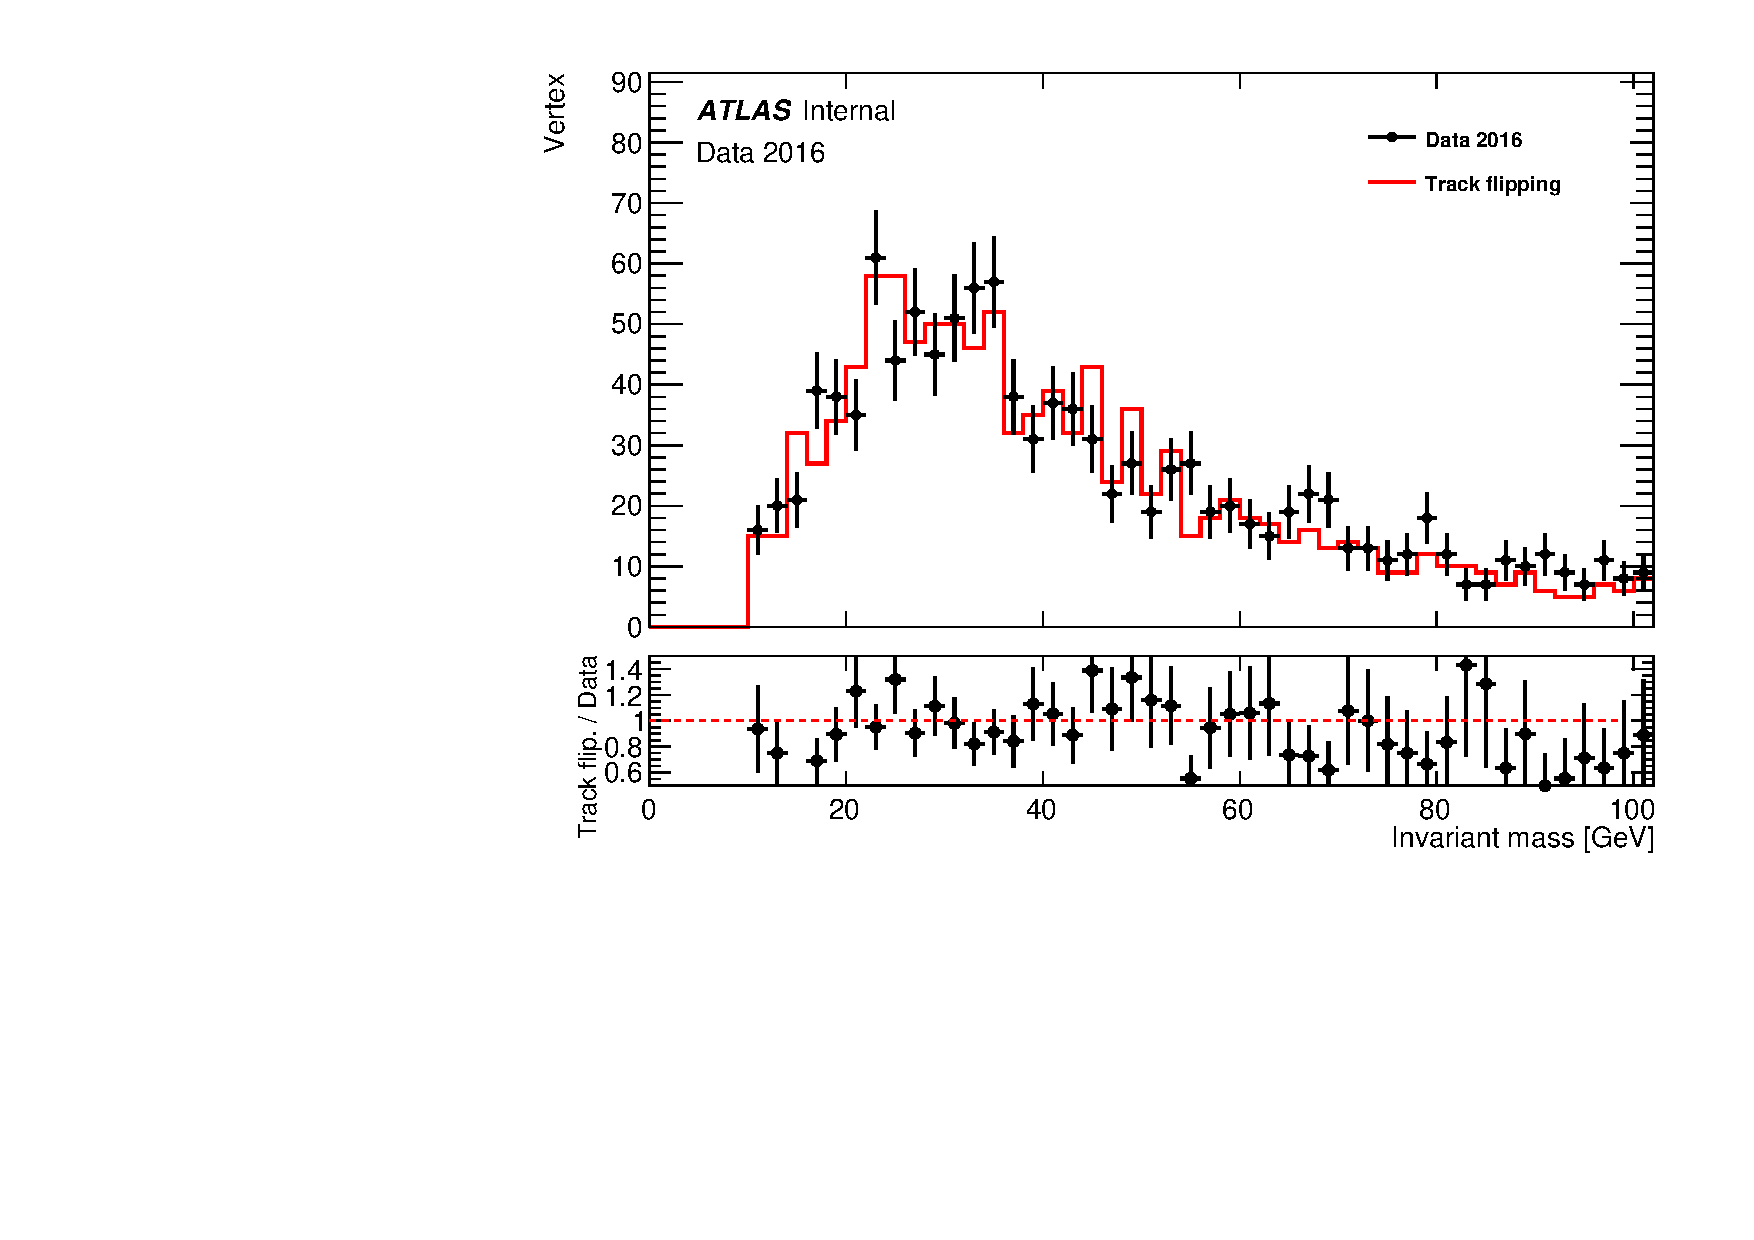
\includegraphics[width=0.45\textwidth]{figures/m_FBE_data_M.pdf}}
    \subfloat[]{\label{subfig:random-crossing_chi2ndof}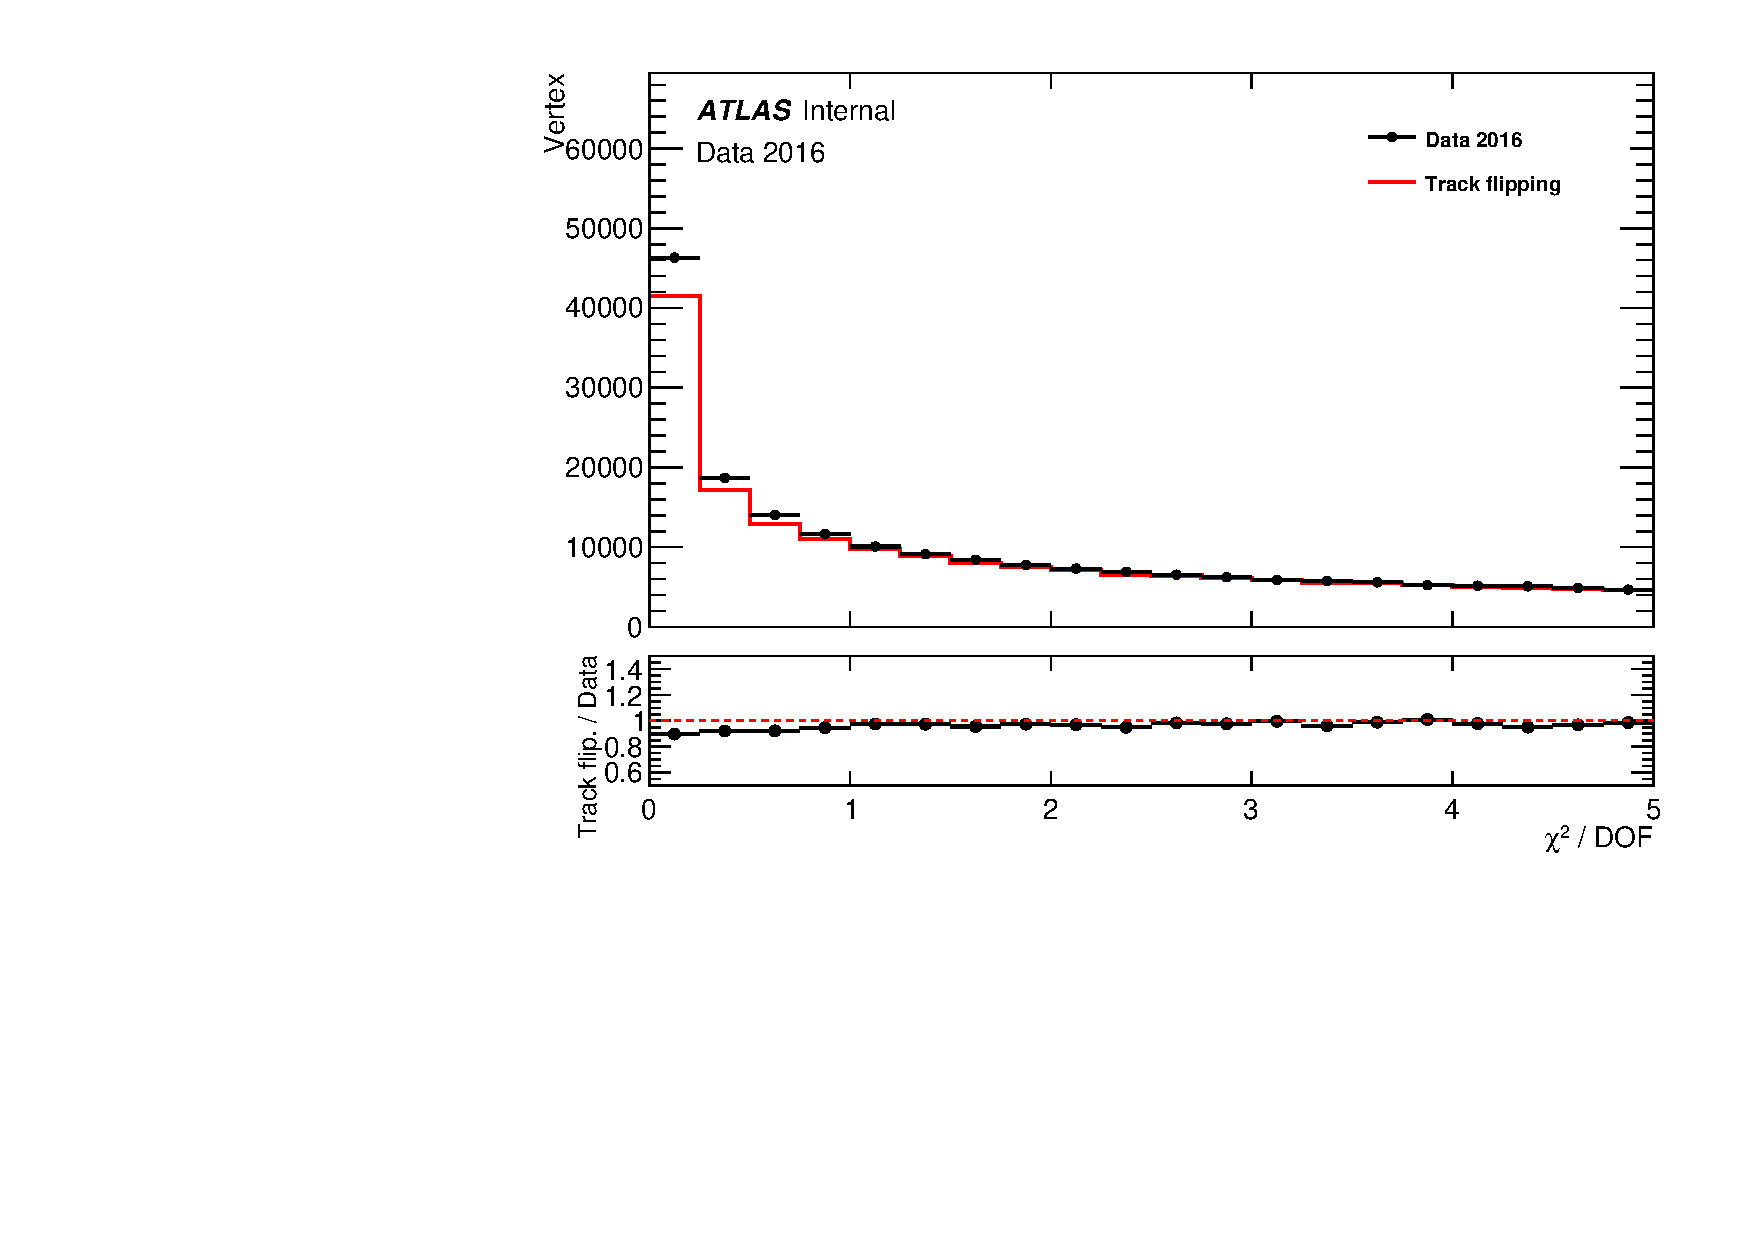
\includegraphics[width=0.45\textwidth]{figures/m_FBE_data_chi2_ndof.pdf}} \\
    \subfloat[]{\label{subfig:random-crossing_r}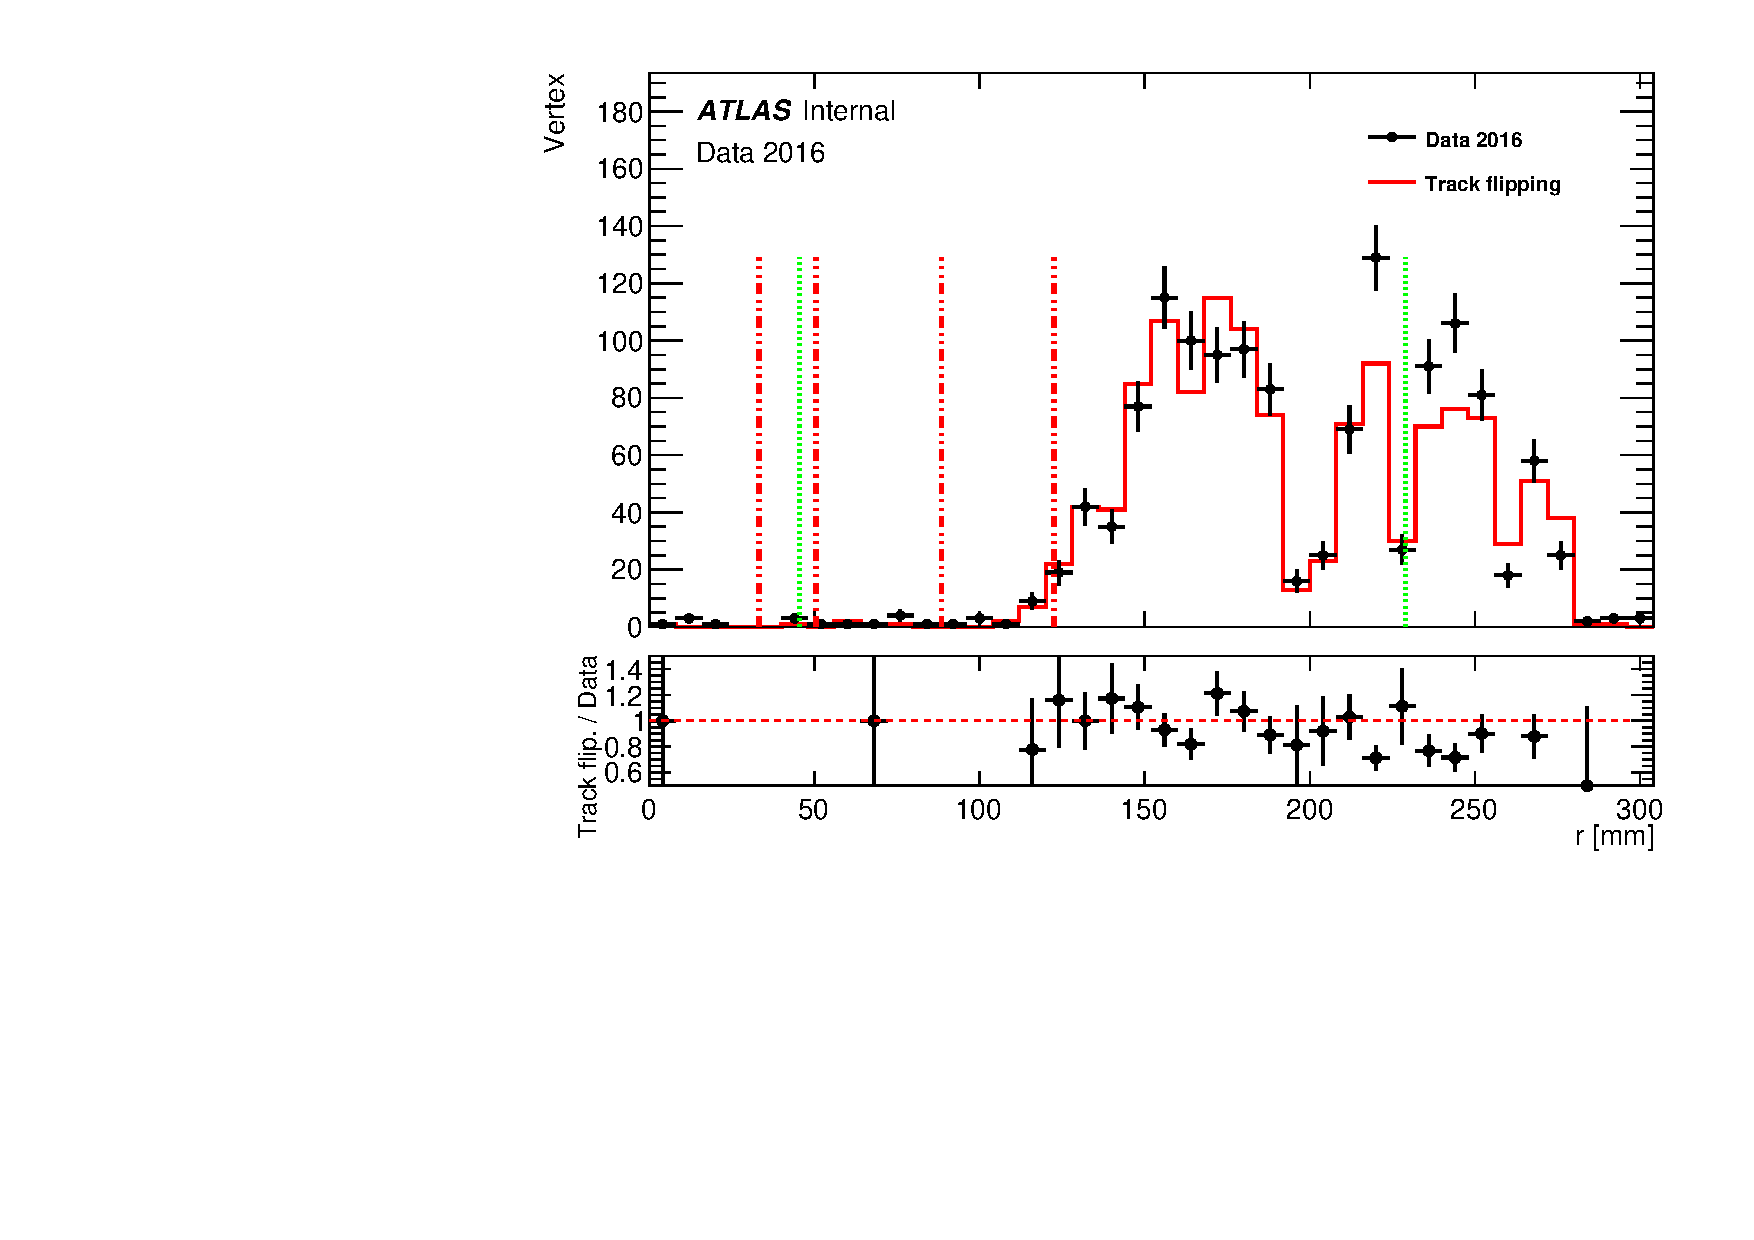
\includegraphics[width=0.45\textwidth]{figures/m_FBE_data_R.pdf}}
    \subfloat[]{\label{subfig:random-crossing_z}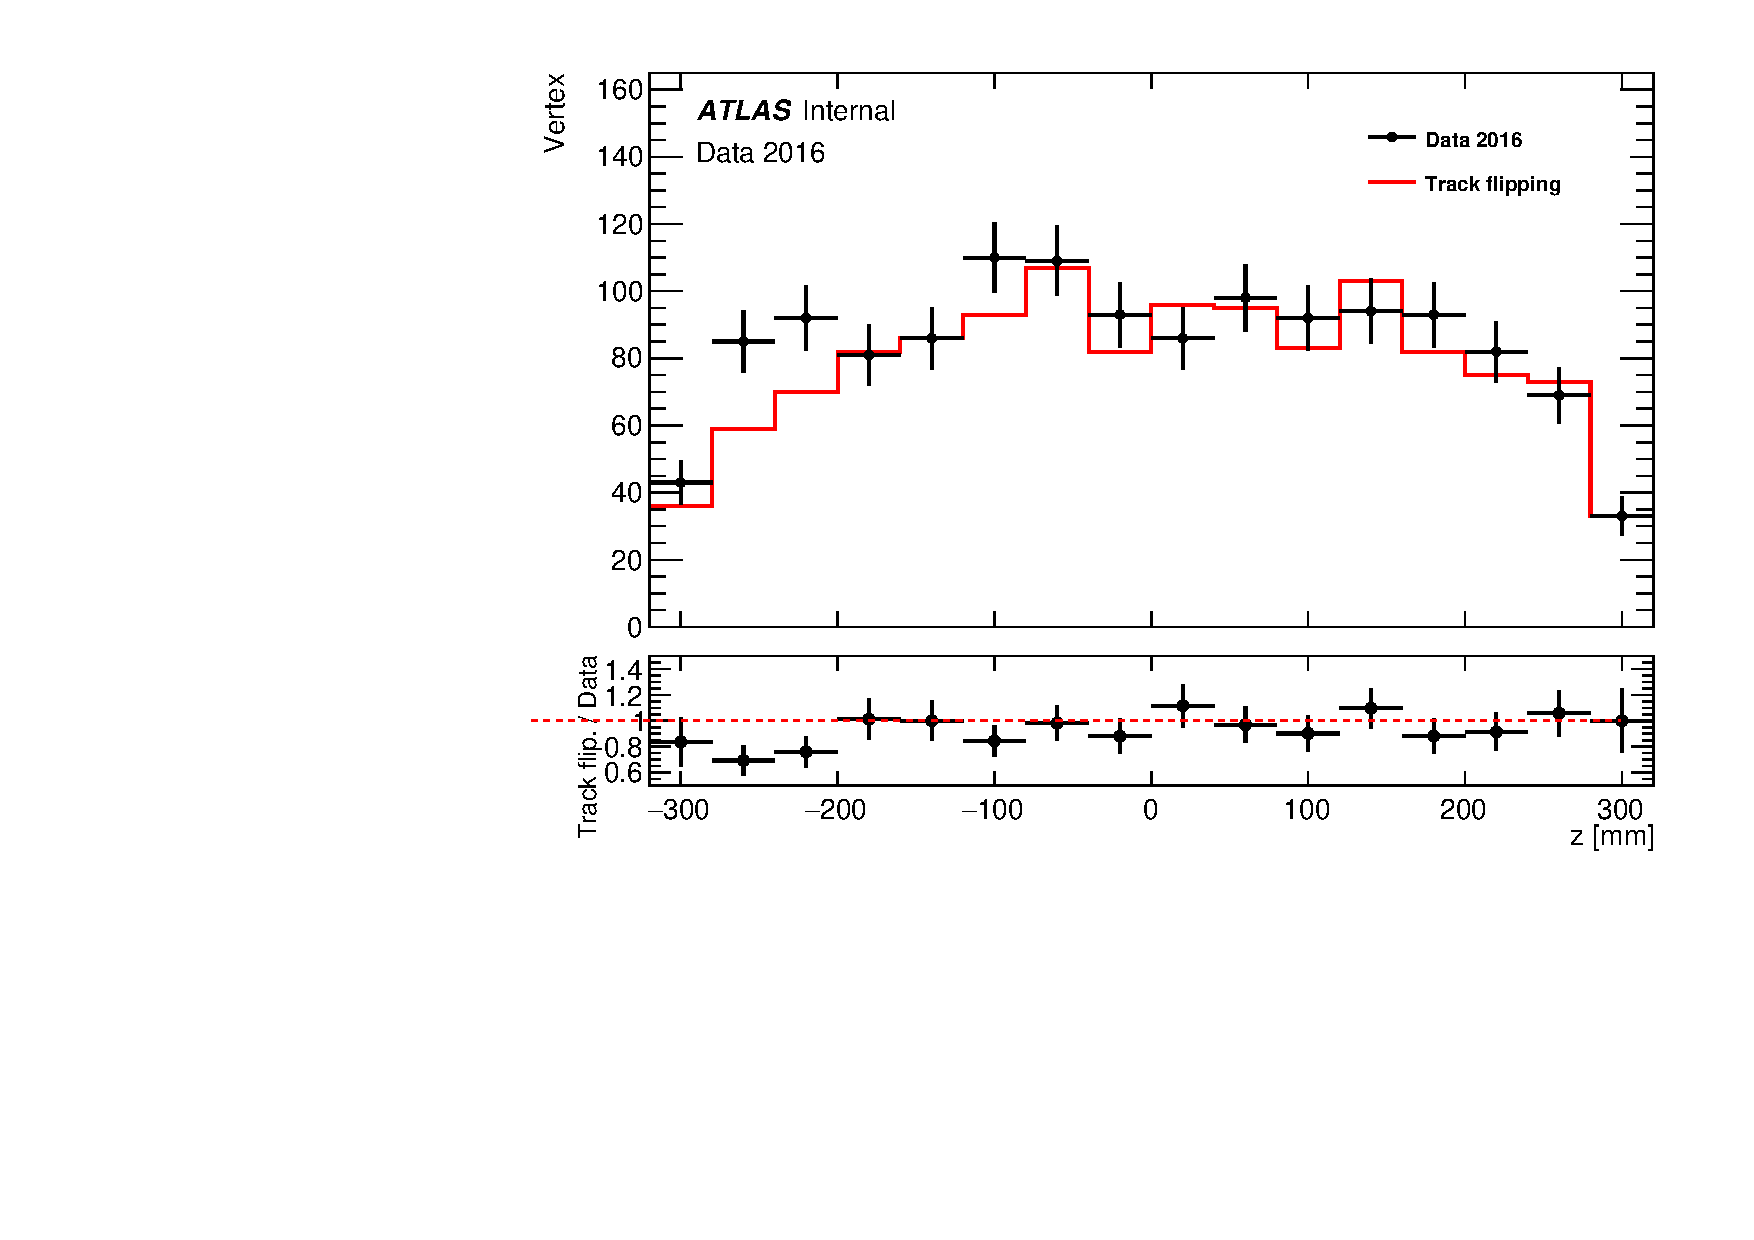
\includegraphics[width=0.45\textwidth]{figures/m_FBE_data_z.pdf}}
    %\subfloat[l]{\label{subfig:random-crossing_l}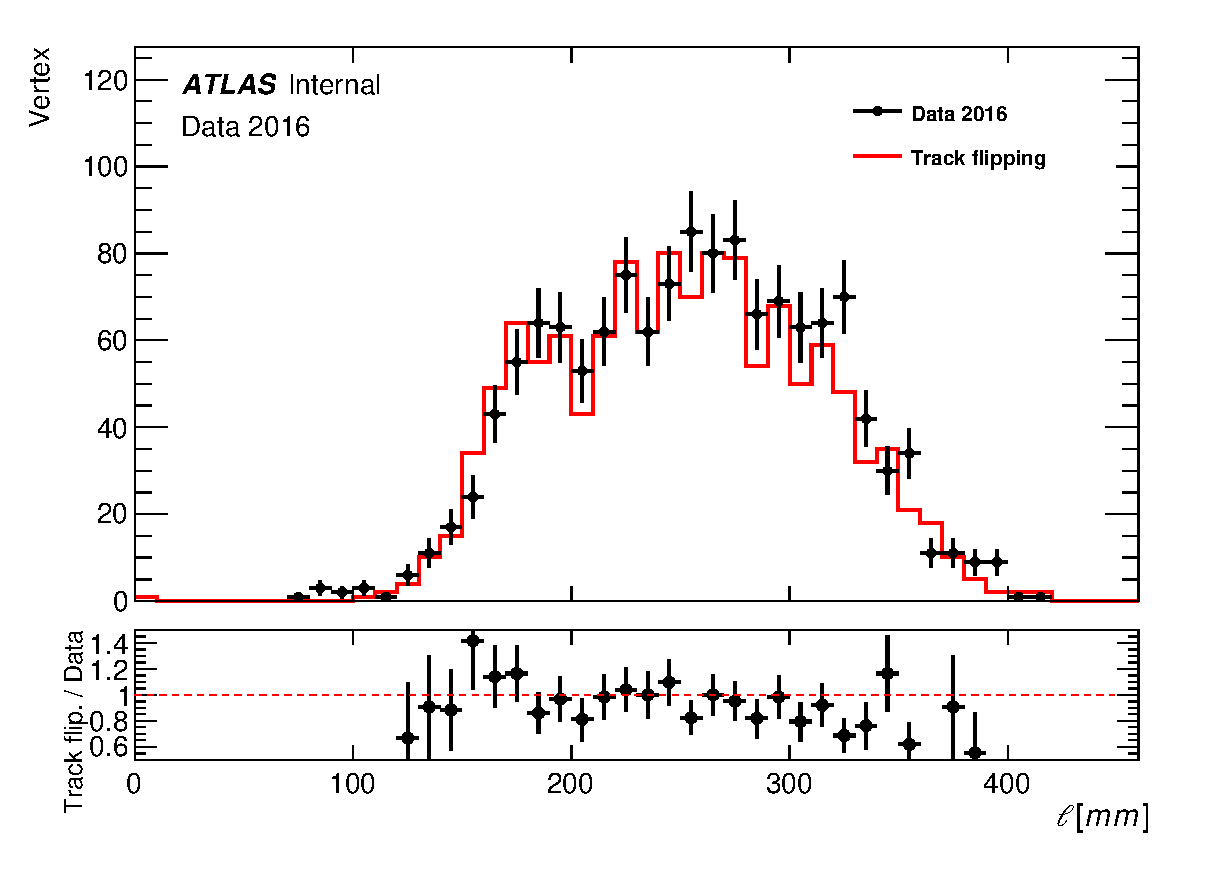
\includegraphics[width=0.45\textwidth]{figures/m_FBE_data_l.eps}}
    \caption{Comparison of (a) vertex mass, (b) $\chi^{2} / \mathrm{DOF}$, (c) transverse, and (d) longitudinal position of vertex found in 32.8 $\mathrm{fb^{-1}}$ of 2016 data sample with those found from the track flipping in the control region of the data sample. In (c), the red dashed lines indicate the four Pixel layers and the first layer of SCT. The green dotted lines indicate the Inner Support Tube (45.5 mm) and Pixel Support Tube (229 mm).}
    \label{fig:random-crossing_vertex_dist_data}
\end{figure}

 Because of the limited statistics in lepton pairs in the data sample, track-flipping vertex yields in the signal region cannot be directly used as random-crossing background estimation. Instead, track-flipping vertex yields in the control region and validation region are extrapolated to estimate random-crossing background in the signal region using lepton probability, defined as follows:
\begin{itemize}
\item $P(e)$ is defined as the ratio of electrons to inner detector tracks in an entire sample,
\item $P(\mu)$ is defined as the ratio of muons to inner detector tracks in an entire sample,
\end{itemize}
where track requirements described in Section~\ref{sec:random_crossing_MC} is required to both leptons and inner detector tracks.

\textbf{Extrapolation from control region} The track-flipping vertex yields in the control region is extrapolated to the signal and validation regions to estimate vertex yields using Eq.~\ref{eq:TF_extrapolation_from_control}. The estimated $\mu x$ and $ex$ vertex yields are compared with the observed track-flipping vertex yield in validation region to calculate scale factors. The scale factor estimated from the extrapolation $xx\rightarrow \mu x$ ($xx\rightarrow ex$) is 0.82 (0.19). The estimated scale factors are applied to the extrapolation to the signal region using Eq.~\ref{eq:TF_scale_factors} to obtain the random-crossing background estimation.

\textbf{Extrapolation from validation region} Similarly, the track-flipping vertex yields in the validation region is extrapolated to the signal to estimate vertex yields using Eq.~\ref{eq:TF_extrapolation_from_validation}. The scale factors are applied to the extrapolation to obtain the background estimation.

The lepton probability, track-flipping and reconstructed vertex yields, scale factors, and estimated random-crossing background are summarized in Table~\ref{table:track_flipping}.

\begin{table}[!htb]%
  \centering
  \subfloat[Lepton probability]{
    \begin{tabular}[t]{ccc}
        \hline\hline
                & Tracks             & P($\ell$)           \\
         \hline
         x      & $2.47\times10^{7}$ & -                   \\
         $\mu$  & $5.23\times10^{4}$ & $2.10\times10^{-3}$ \\
         $e$    & $3.63\times10^{4}$ & $1.46\times10^{-3}$ \\
         Sum    & $2.48\times10^{7}$ & - \\
        \hline\hline
    \end{tabular}
  }%
  \qquad
  \subfloat[Vertex yields]{
    \begin{tabular}[t]{ccc}
        \hline\hline
                & Tracks-flipping    & Data                \\
         \hline
         $xx$   & 1255               & 1346                \\
         $\mu x$& 3                  & 4                   \\
         $ex$   & 1                  & 0                   \\
        \hline\hline
    \end{tabular}
  }%
  \qquad
  \subfloat[Scale factors]{
    \begin{tabular}[t]{cc}
        \hline\hline
         Type                      & SF      \\
         \hline
         $S_{xx\rightarrow\mu x}$  & 0.82              \\
         $S_{xx\rightarrow ex}$    & 0.19              \\
        \hline\hline
    \end{tabular}
  }%

  \subfloat[Extrapolation from control region]{
    \begin{tabular}[t]{ccc}
        \hline\hline
                         & Estimation          & Applying SF         \\
         \hline
         $N_{\mu x}$     & 4                   & -                   \\
         $N_{e x}$       & 5                   & -                   \\
         $N_{\mu\mu}$    & $2.69\times10^{-3}$ & $1.79\times10^{-3}$ \\
         $N_{ee}$        & $5.56\times10^{-3}$ & $1.99\times10^{-4}$ \\
         $N_{e\mu}$      & $7.73\times10^{-3}$ & $1.96\times10^{-3}$ \\
        \hline\hline
    \end{tabular}
  }%
  \qquad
  \subfloat[Extrapolation from validation region]{
    \begin{tabular}[t]{ccc}
        \hline\hline
                         & Estimation          & Applying SF         \\
         \hline
         $N_{\mu\mu}$    & $2.19\times10^{-3}$ & $1.79\times10^{-3}$ \\
         $N_{ee}$        & $1.05\times10^{-3}$ & $1.99\times10^{-4}$ \\
         $N_{e\mu}$      & $3.89\times10^{-3}$ & $1.96\times10^{-3}$ \\
        \hline\hline
    \end{tabular}
  }%
  
  \caption{Random-crossing background by track flipping}%
  \label{table:track_flipping}
\end{table}

\subsubsection{Systematic uncertainty in the track flipping method}
\label{sec:random_crossing_systematics}

The systematic uncertainty in the track flipping method is estimated by studying the variance in background estimation from different variations of the track flipping method. In addition to the transformation described in the previous section ($d_{0}\rightarrow -d_{0}, z_{0}\rightarrow -z_{0}, \phi\rightarrow\phi-\pi, \theta\rightarrow\pi-\theta$), the following track transformations are considered.
\begin{itemize}
\item \textbf{Same sign d0}: $d_{0}\rightarrow d_{0}, z_{0}\rightarrow -z_{0}, \phi\rightarrow\phi-\pi, \theta\rightarrow\pi-\theta$
\item \textbf{Same sign $\theta$}: $d_{0}\rightarrow -d_{0}, z_{0}\rightarrow -z_{0}, \phi\rightarrow\phi-\pi, \theta\rightarrow\theta$
\item \textbf{90 degrees rotation in $\phi$}: $d_{0}\rightarrow -d_{0}, z_{0}\rightarrow -z_{0}, \phi\rightarrow\phi-\frac{\pi}{2}, \theta\rightarrow\theta$
\end{itemize}


\textbf{NEED TO ADD RESULTS HERE}

\newpage






\subsection{Cosmic background}
\label{sec:cosmic_ray}
Cosmic background is the dominant source of backgrounds in $\mu\mu$ channel as a cosmic muon can be reconstructed as a back-to-back $\mu\mu$ vertex with large displacement from the primary vertex. Cosmic veto is introduced to suppress the background from such vertices by requiring $R_{\mathrm{CR}} = \sqrt{(\Delta \phi - \pi)^{2} + (\Sigma \eta)^{2}} >$ 0.04 where $\Delta \phi$, $\Sigma \eta$ are the difference and sum of track parameters from two tracks at a vertex, respectively. For a back-to-back vertex, $R_{\mathrm{CR}}$ is expected to be close to 0. The vertex cut flow in Figure~\ref{fig:signal_cutflow_MC_mumu} shows that the efficiency loss due to the cosmic veto is negligible.

In order to estimate the cosmic background, \textit{cosmic control region} is defined by inverting the cosmic veto cut (i.e. $R_{CR} < 0.04$). All other event and vertex selections are kept the same as the signal region. Figure~\ref{subfig:cosmic_cutflow} shows the vertex cut flow of the cosmic control region in the data sample. There are 127 $\mu\mu$ vertices found with $R_{CR} < 0.04$, and no $ee$ or $e\mu$ vertex was found. Figure~\ref{subfig:cosmic_Rcr} shows the $R_{CR}$ distribution of these vertices. All vertices found in the cosmic control region have very small $R_{CR}$. The $R_{CR}$ distribution is fitted with gaussian function and then extrapolated into the signal region, and the cosmic background is estimated to be negligible.


%and the extrapolation of the fit estimates that the cosmic background in the signal region is less than $10^{-19}$.
% Pairs of muon tracks found in data that satisfies $R_{CR} < 0.04$ are shown as an upper bound of $\mu\mu$ vertex yields.
%The exponential distribution suggests that no cosmic muon background is expected in the signal region.

%The extrapolation of the exponential fit to $R_{CR}$ distribution of $\mu\mu$ vertex estimates that the cosmic muon background in the signal region is less than $10^{-19}$.


\begin{figure}[!htb]
    \centering
    \subfloat[]{\label{subfig:cosmic_cutflow}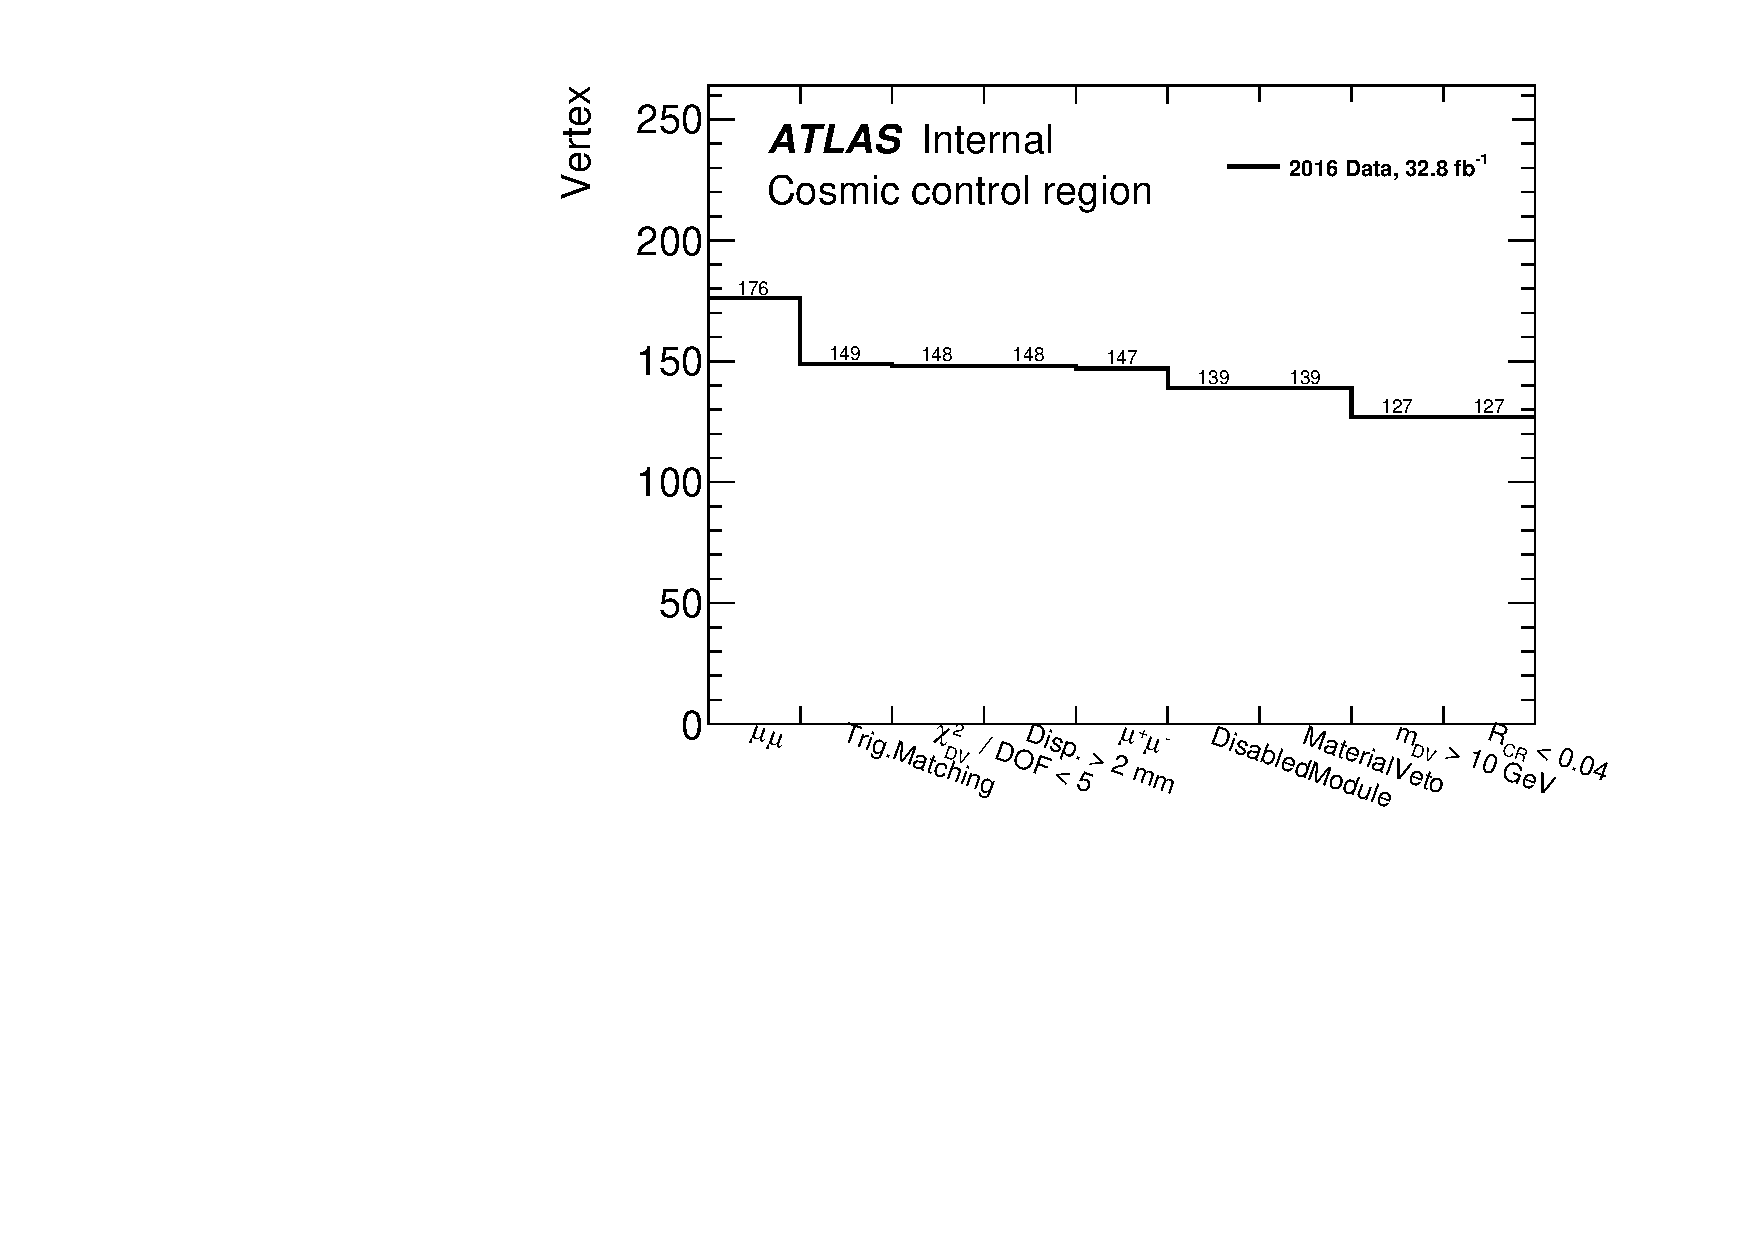
\includegraphics[width=0.50\textwidth]{figures/m_data_cosmic_vertex_cutflow_mumu.pdf}}
    \subfloat[]{\label{subfig:cosmic_Rcr}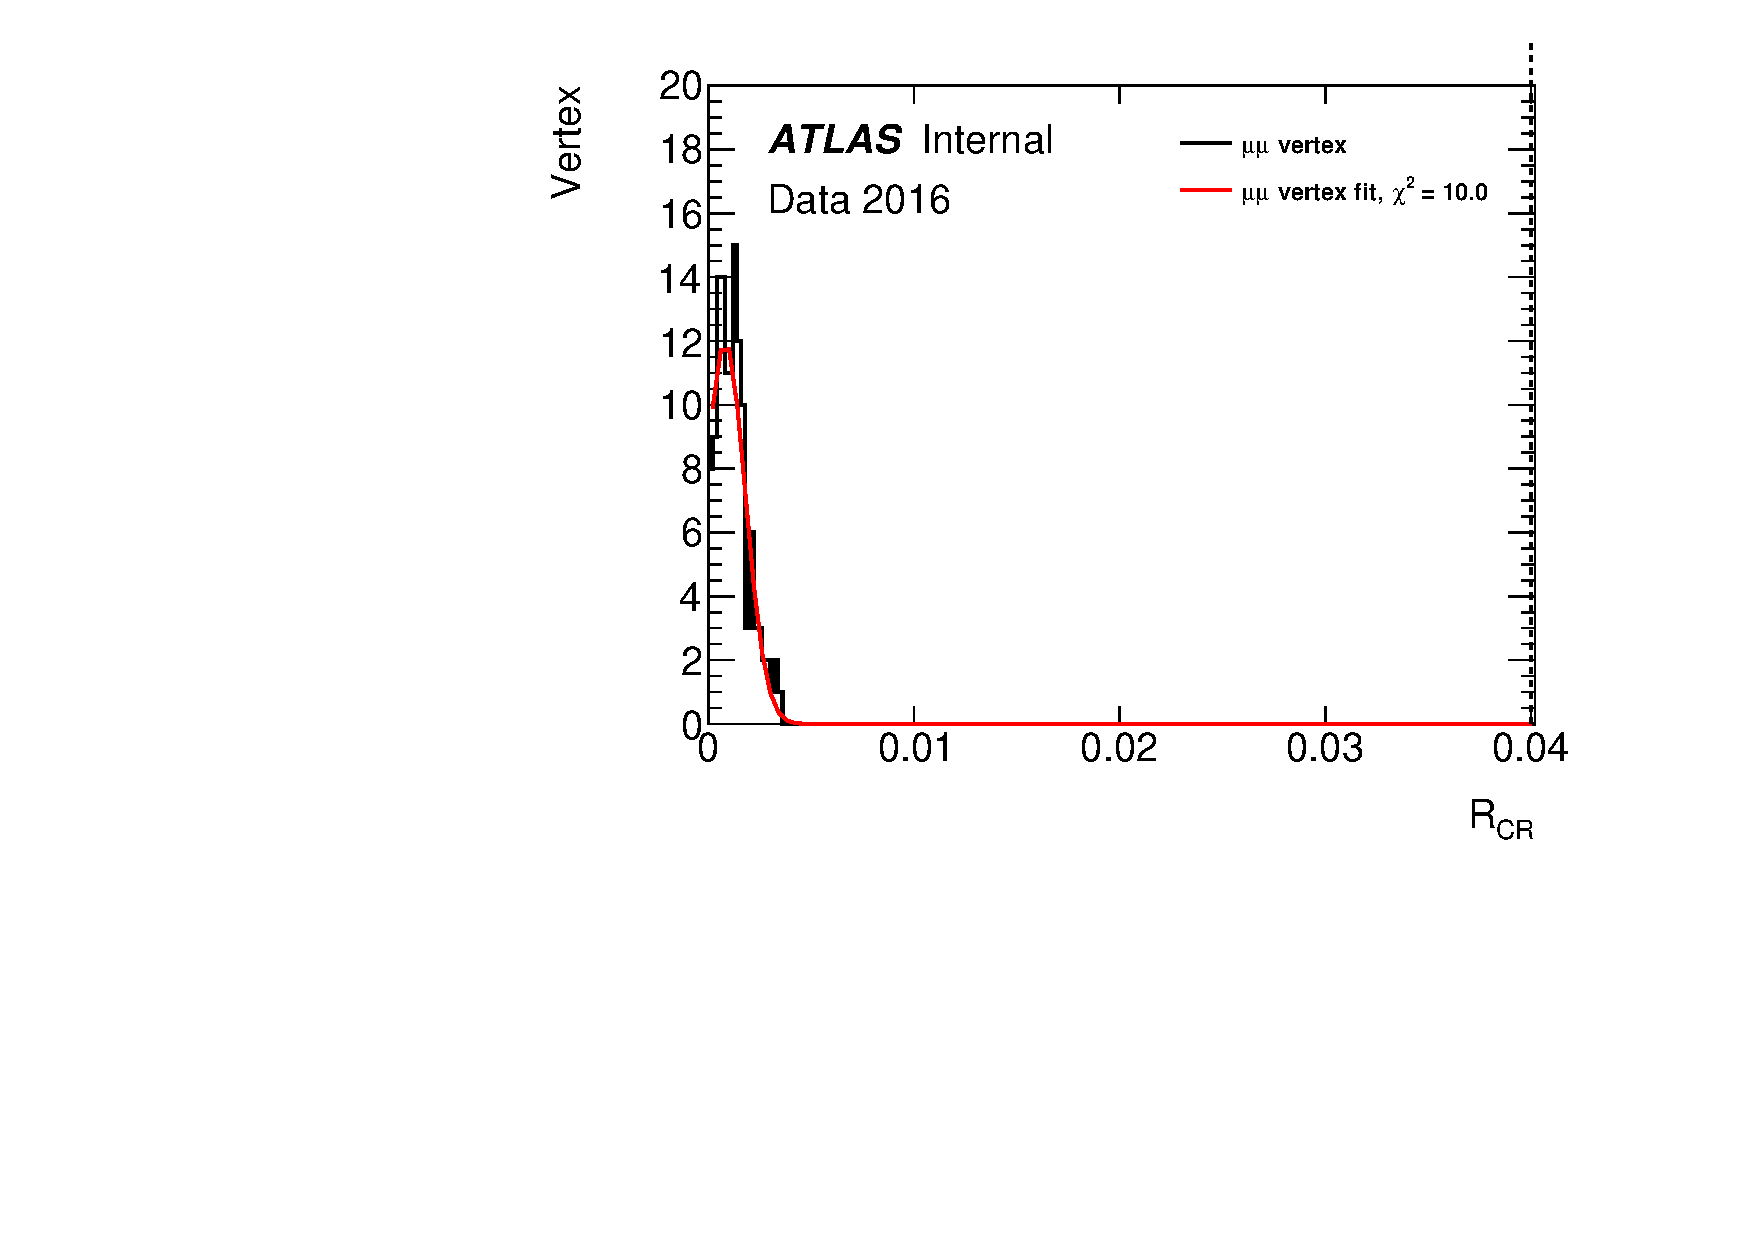
\includegraphics[width=0.50\textwidth]{figures/m_cosmic_background.pdf}}
    \caption{(a) Vertex cut flow of the cosmic control region, and (b) $R_{CR}$ distribution of $\mu\mu$ vertex found in the data sample. The curve shows a fit with an exponential function.}
    \label{fig:cosmic_control}
\end{figure}


\subsection{Low-mass background}
\label{sec:low_mass}
A SM process such as photon conversion or the decay of a low-mass particle, e.g. $J/\psi$, can be reconstructed as a low-mass, displaced vertex decaying to a dilepton final state. Low-mass veto is implemented to suppress background from these displaced vertices ($m > 10$ GeV). Due to large mass of $Z'$ in the signal MC samples, there is no efficiency loss by the veto.

\textit{Low-mass control region} is used to estimate the low-mass background by inverting the low-mass cut (i.e. $m < 10$ GeV). All other event and vertex selections are kept the same as the signal region. 

Figure~\ref{fig:lowmass_control} shows the vertex cut flow and mass distribution of the vertices found in the low-mass control region in the data. There are 12 vertices with $m < $ 10 GeV, passing all other signal selections. The mass spectrum is fitted with the sum of a Gaussian centered around $3$ GeV, representing $J/\psi$ resonance, and an exponential for the background distribution. The extrapolation of the combined fit yields an estimate of $\backsim 0.09$ vertices in the signal region.
%The $R_{CR}$ distribution of $\mu\mu$ vertex is fitted with an exponential, extrapolated into the signal region yielding an estimate of $10^{-19}$ vertices.



\begin{figure}[!htb]
    \centering
    \subfloat[]{\label{subfig:lowmass_cutflow}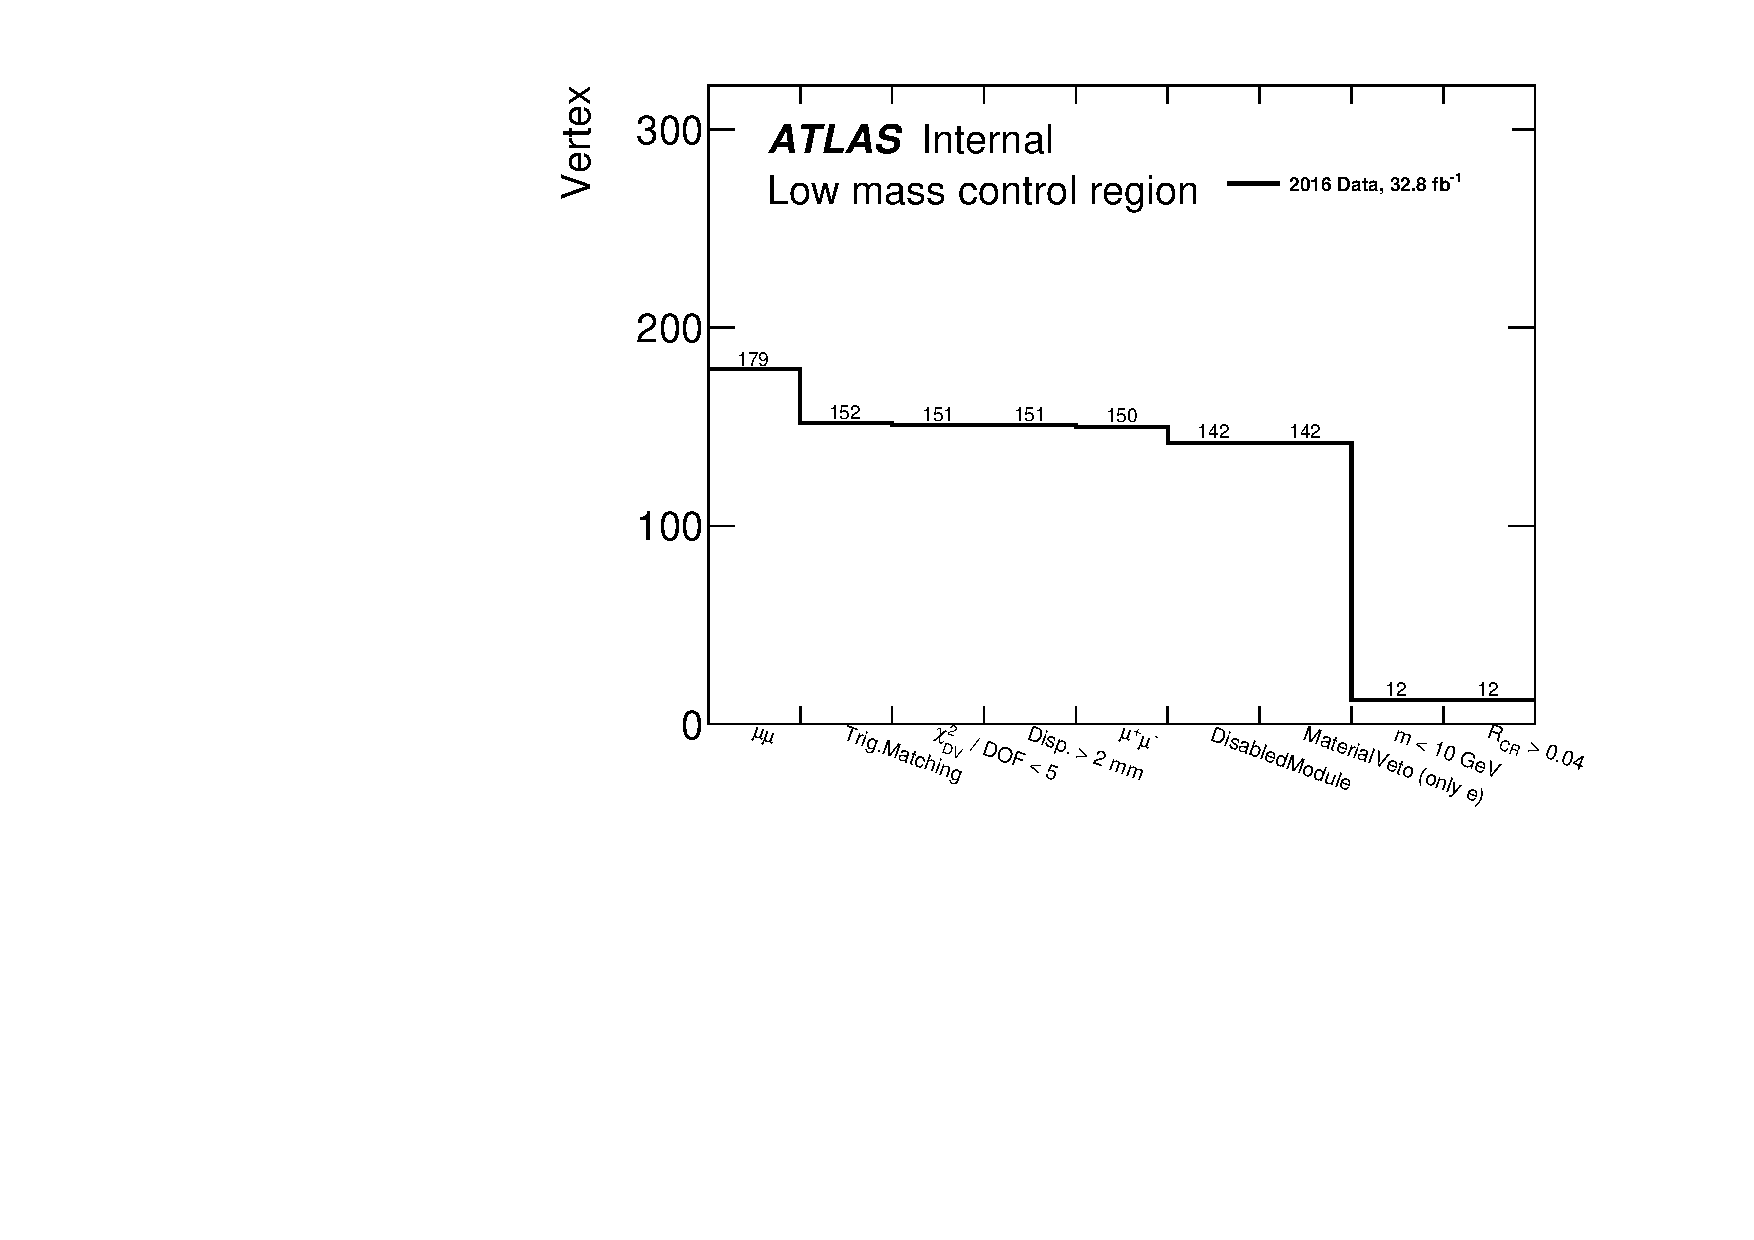
\includegraphics[width=0.50\textwidth]{figures/m_data_dv_cutflow_lowmass_mumu.pdf}}
    \subfloat[]{\label{subfig:lowmass_dist}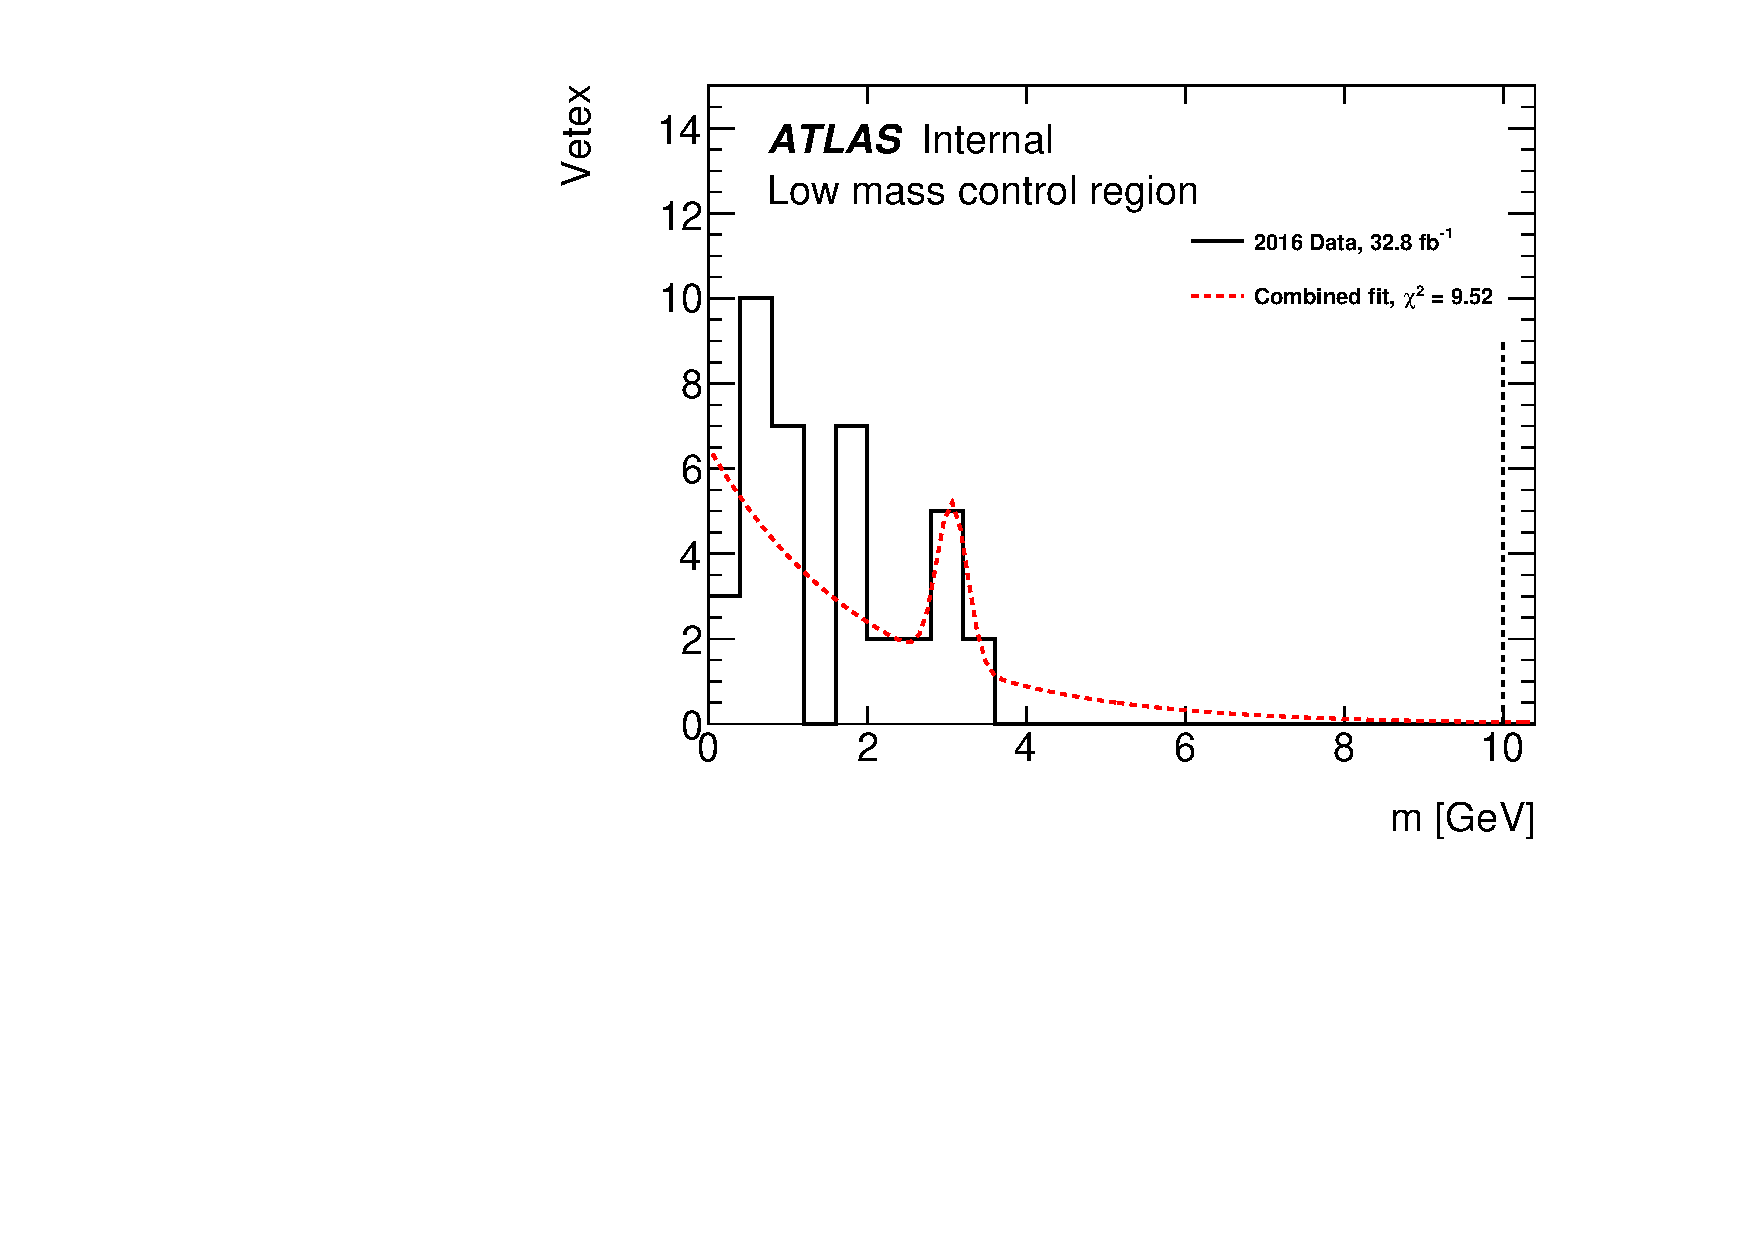
\includegraphics[width=0.50\textwidth]{figures/m_data_dv_mumu_M_low.pdf}}
    \caption{(a) Vertex cut flow and (b) mass distribution of the low-mass control region from the data sample. The combined fit of a Gaussian centered around $3$ GeV, representing $J/\psi$ resonance, and an exponential for the background is used to estimate the low-mass background in the signal region.}
    \label{fig:lowmass_control}
\end{figure}





%-------------------------------------------------------------------------------
\section{Systematic uncertainties}
\label{sec:syst}
The systematic uncertainty in the signal efficiency is estimated by estimating the systematic uncertainty of each efficiency factor in Eq.~\ref{eq:OverallEff}.

The systematic uncertainties on $\varepsilon_{\mathrm{track}}$, $\varepsilon_{\mathrm{vertexTrack}}$, and $\varepsilon_{\mathrm{vertexFit}}$ are studied using $K_{S}$ in Section~\ref{sec:syst_vertexing}. The systematic uncertainties on $\varepsilon_{\mathrm{lepton}}$ is studied in Section~\ref{sec:syst_leptonID} using tag-and-probe method with $Z\rightarrow ee,\mu\mu$ events. The systematic uncertainties on $\varepsilon_{\mathrm{trigger}}$ and $\varepsilon_{\mathrm{filter}}$ will be studied separately.

\subsection{Systematic uncertainties on tracking and vertexing efficiency}
\label{sec:syst_vertexing}
\subsubsection{Data and MC comparison}
\label{sec:vertexing_systematics_data_MC}
The systematic uncertainties on $\varepsilon_{\mathrm{track}}$, $\varepsilon_{\mathrm{vertexTrack}}$, and $\varepsilon_{\mathrm{vertexFit}}$ are estimated by comparing the tracking and vertexing efficiencies between the data and the background MC samples described in Section~\ref{sec:data_sample} using the process, $K_{S}\rightarrow\pi^{+}\pi^{-}$. In order to understand the validity and the limitation of this method, the kinematic distributions of $K_{S}$ and $Z'$ found in this method are compared in Appendix~\ref{app:syst_Ks_Zp}.

%In order to estimate the systematic uncertainties in reconstructing a displaced vertex, the tracking and vertexing efficiencies are compared between the data and the background MC samples described in Section~\ref{sec:data_sample} using $K_{S}\rightarrow\pi^{+}\pi^{-}$. % and its long lifetime ($c\tau \approx 26.84$ mm).

%The $K_{S}$ efficiency can be written as Eq.~\ref{eq:KaonEff}
%\begin{equation}
%\label{eq:KaonEff}
%\varepsilon_{K_{S}}=(\varepsilon_{\mathrm{track}}\cdot\varepsilon_{\mathrm{vertexTrack}})^2\cdot\varepsilon_{\mathrm{vertexFit}}=\bigg(\frac{N_{\mathrm{track}}}{N_{K_{S}}}\cdot\frac{N_{\mathrm{vertexTrack}}}{N_{\mathrm{track}}}\bigg)^2\cdot\frac{N_{\mathrm{vertex}}}{N_{\mathrm{trackPair}}}
%\end{equation}

Events are selected using the same event selection described in Section~\ref{sec:signal_selection}. %except trigger filter as electron or muon triggers are not useful for $K_{S}$ study. %In data sample, trigger applied?
From the selected events, $K_{S}$ candidates, referred as $K_{S}$ vertices, are selected by applying $K_{S}$ vertex selection to the secondary vertices in the events. $K_{S}$ vertex selection is similar to the $Z'$ signal vertex selection, but for the consistency with $K_{S}$ study in Run I and further background reduction, additional vertex cuts as described in Ref.~\cite{Aad:2011hd} are applied in $K_{S}$ vertex selection. The mass window of 0.35 to 0.65 GeV is used in the $K_{S}$ vertex selection. The difference between $K_{S}$ and $Z'$ vertex selections are summarized in Table~\ref{table:ks_vertex_cut}. Figure~\ref{fig:Ks_vertex_cutflow} shows $K_{S}$ vertex cut flow in the data and the background MC samples.

\begin{table}[!htb]
%\begin{table}[tb]
  \centering
  \begin{tabular}{ c c c }
    \hline
    \hline
    & $Z'$& $K_{S}$ \\
    \hline
    Vertex type & $\mu\mu$, $e\mu$, $ee$ & xx \\
    Mass (GeV) & $> 10.0$ & $[0.35,0.65]$ \\
    Additional cut & - & $K_{S}$ selection~\cite{Aad:2011hd} \\
    \hline
    \hline
  \end{tabular}
  \caption{Comparison of $Z'$ and $K_{S}$ vertex selections.}
  \label{table:ks_vertex_cut}
\end{table}

%\begin{figure}[tb]
\begin{figure}[!htb]
	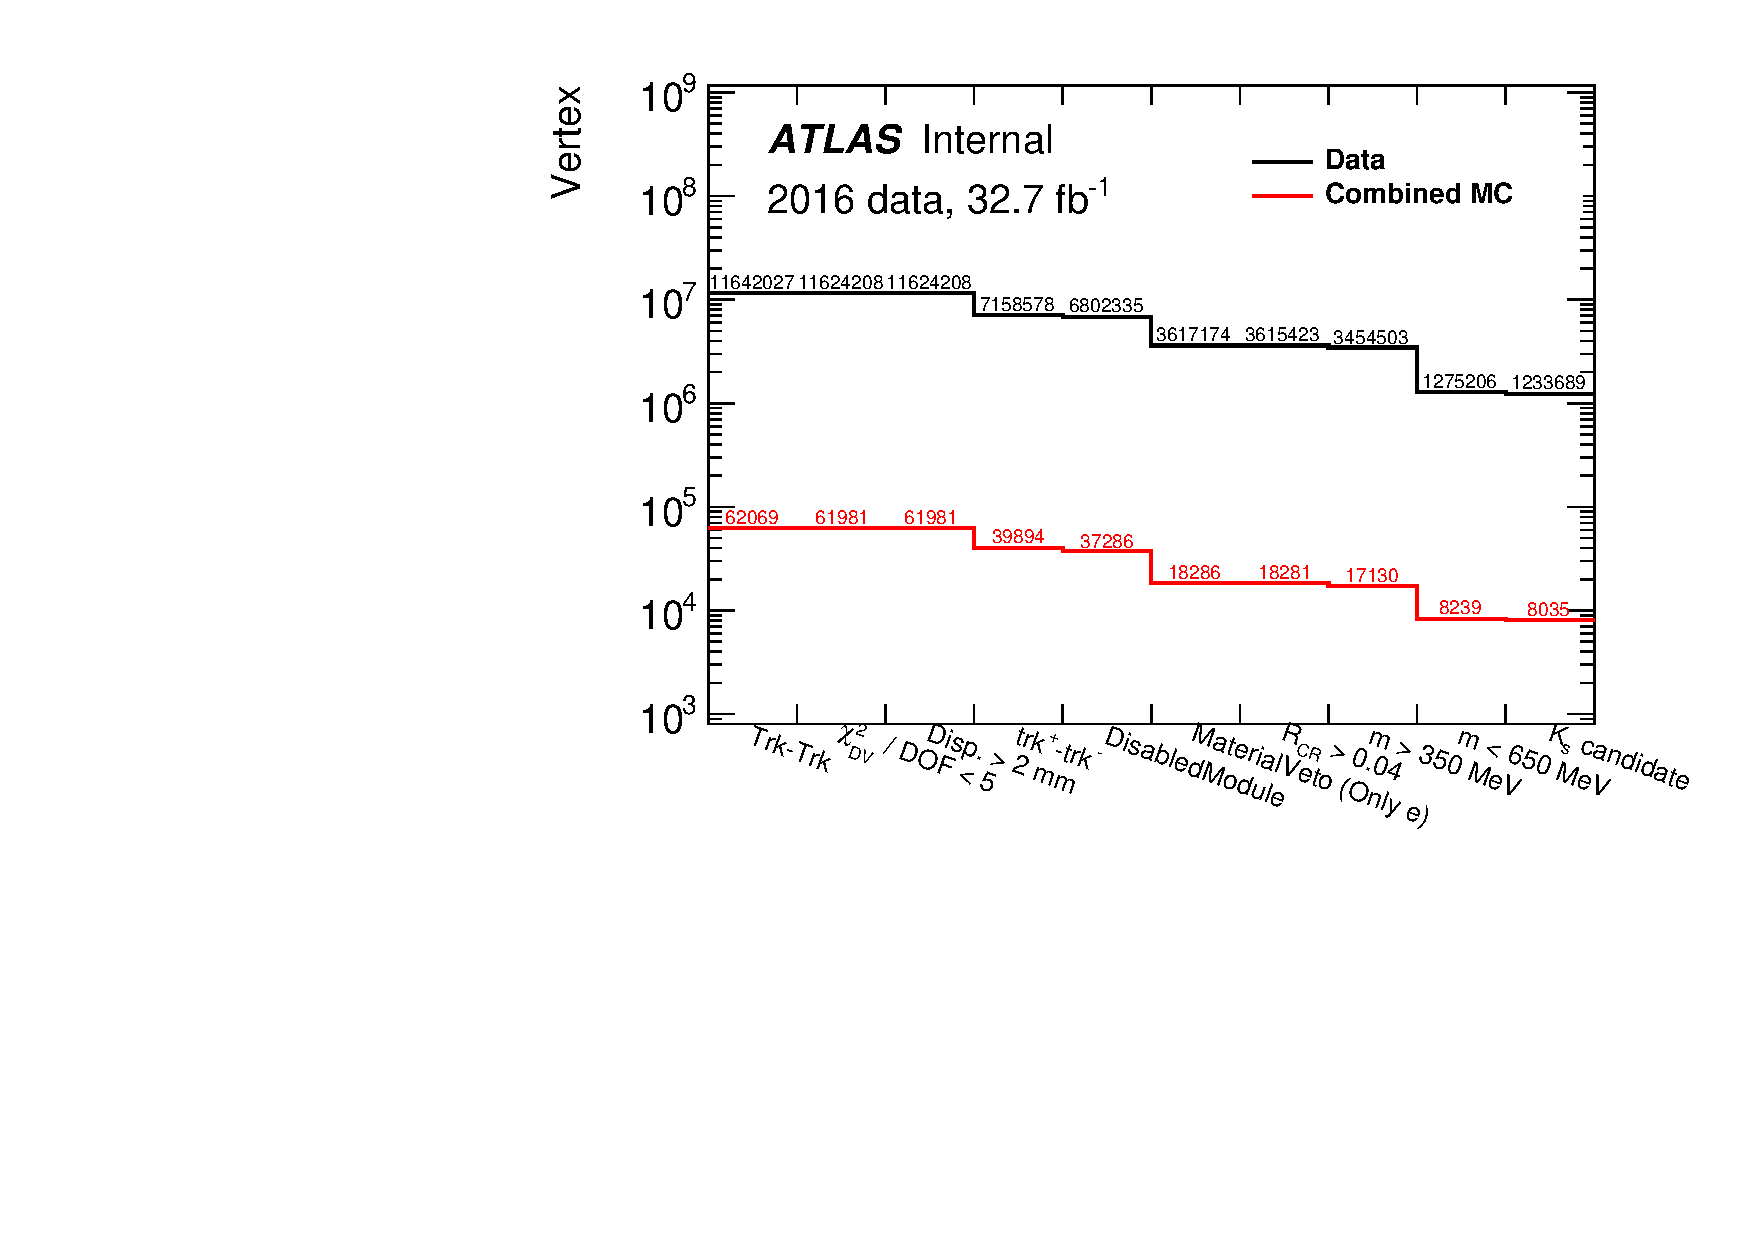
\includegraphics[width=0.60\textwidth]{figures/m_syst_Ks_cf.pdf}
	\centering
	\caption{Vertex cut flow applied on $K_{S}$ vertices in the data and MC samples}
	\label{fig:Ks_vertex_cutflow}
\end{figure}

After applying the event and $K_{S}$ vertex selection, the $K_{S}$ vertex distributions in the data are compared to the MC samples in Figure~\ref{fig:Ks_data_MC}. The data sample is normalized to the MC sample which has limited statistics. There are good agreements in the invariant mass, $p_{T}$, transverse, longitudinal position, and decay length of the vertices, except the pile-up distribution as expected.


\begin{figure}[!htb]
    \centering
    \subfloat[]{\label{subfig:Ks_m}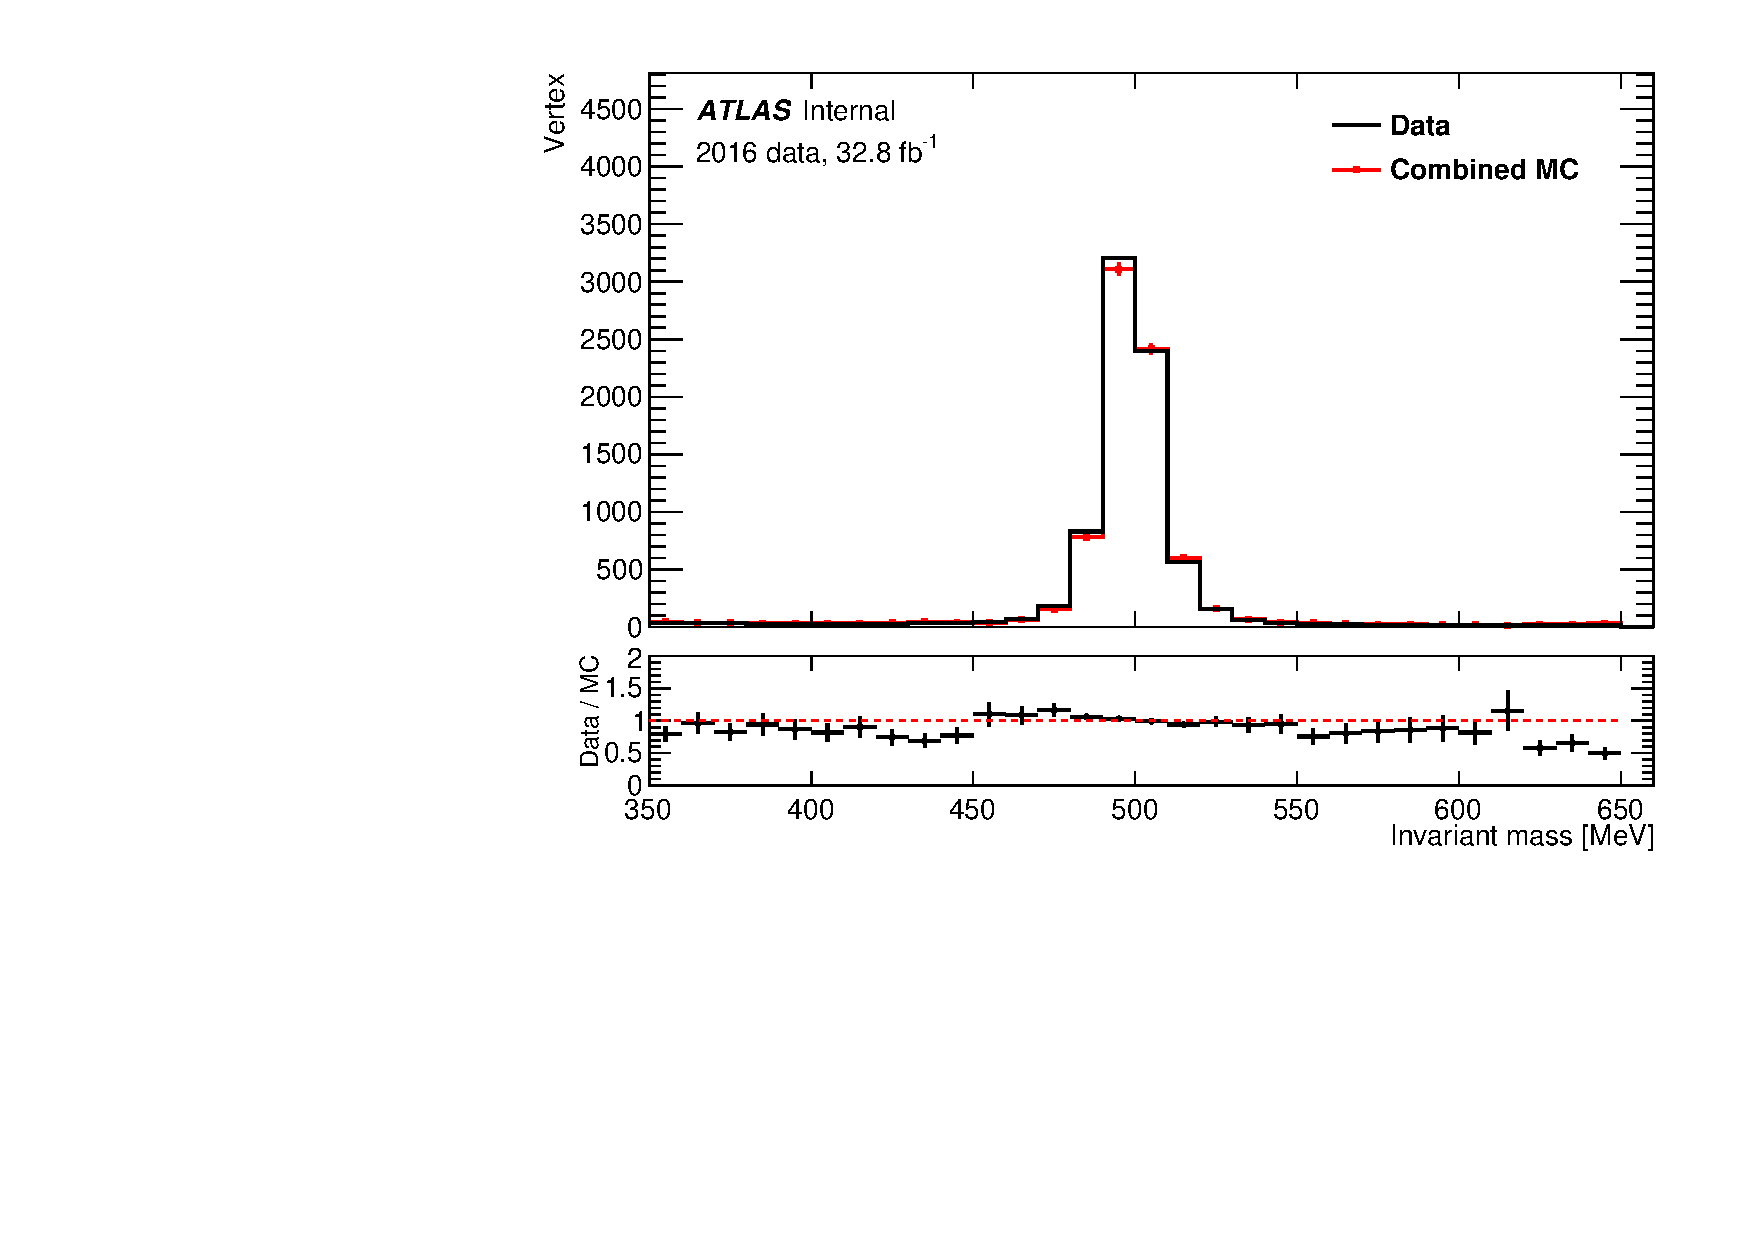
\includegraphics[width=0.45\textwidth]{figures/m_syst_Ks_M.pdf}}
    \subfloat[]{\label{subfig:Ks_pt}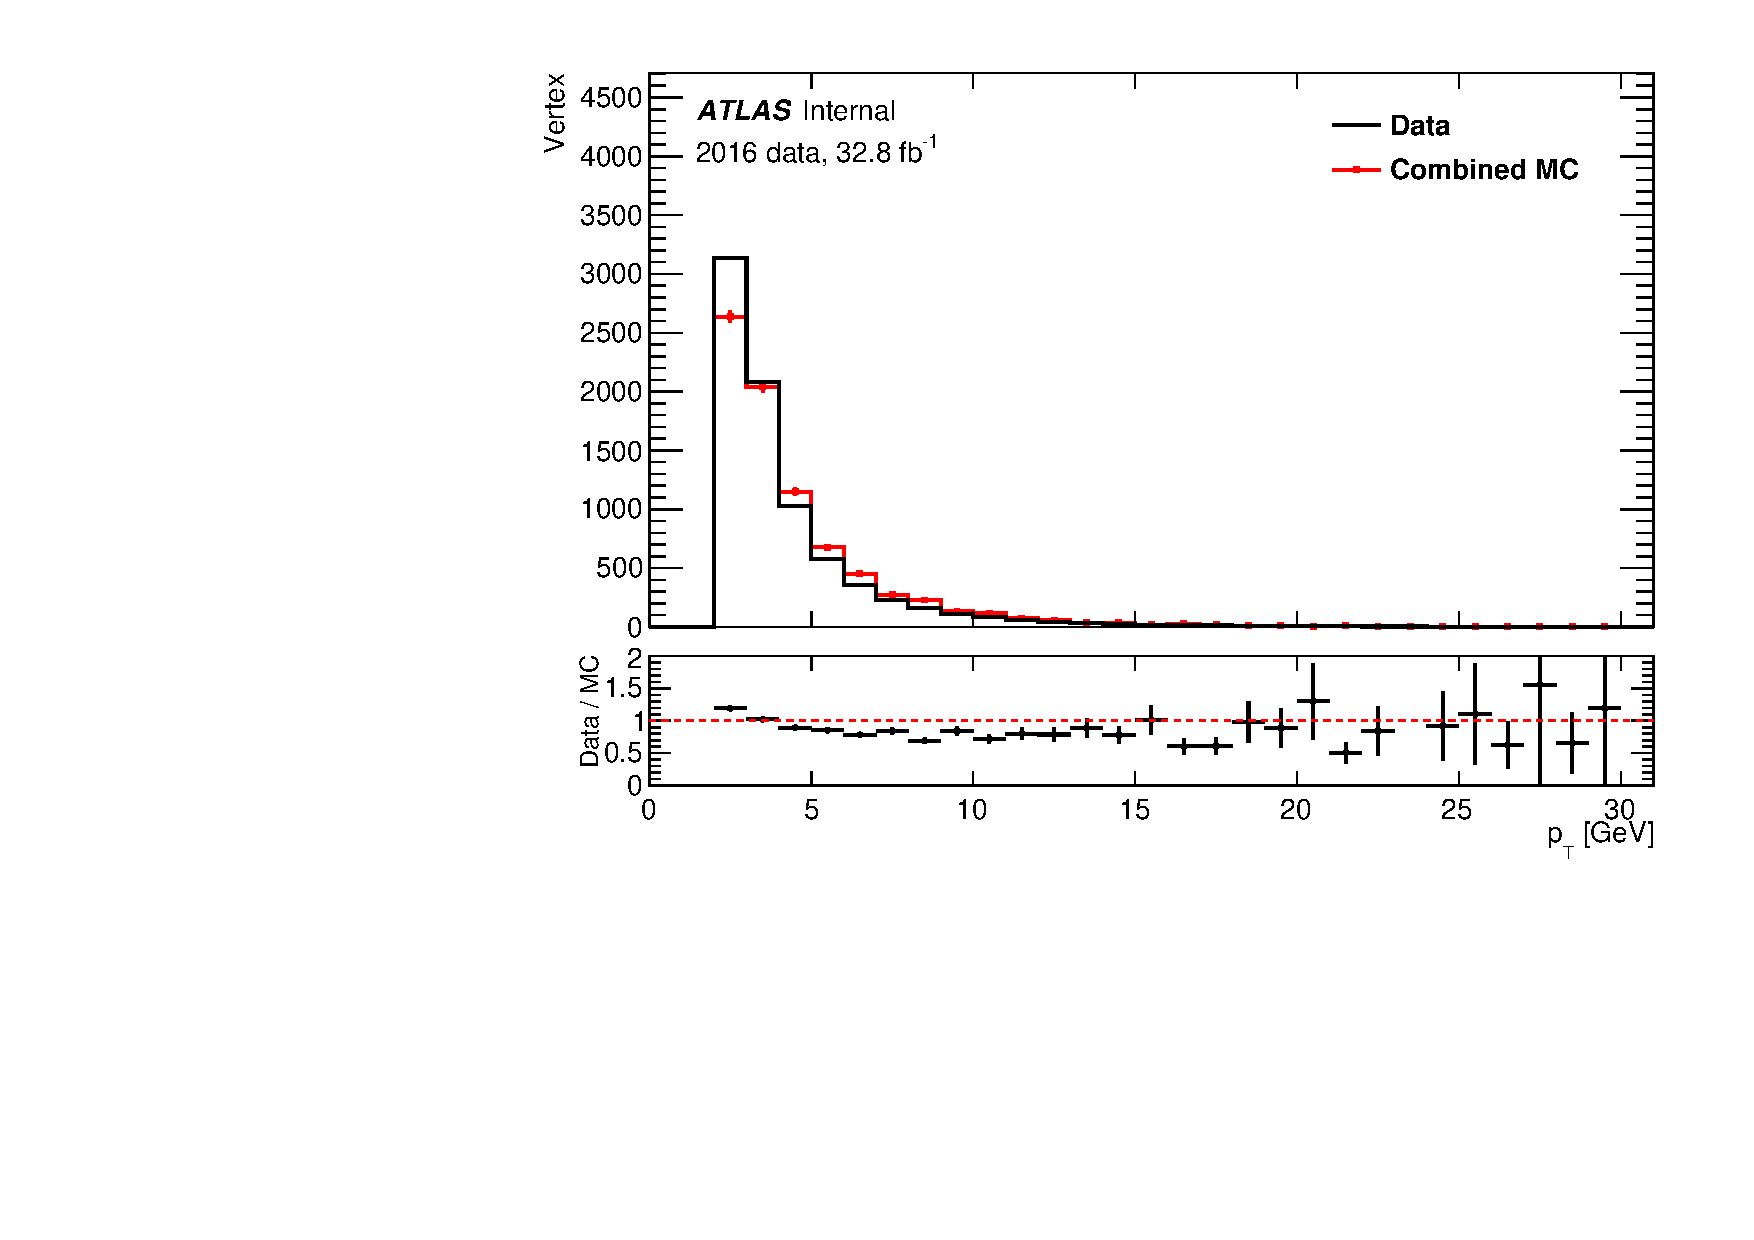
\includegraphics[width=0.45\textwidth]{figures/m_syst_Ks_pt.pdf}} \\
    \subfloat[]{\label{subfig:Ks_mu}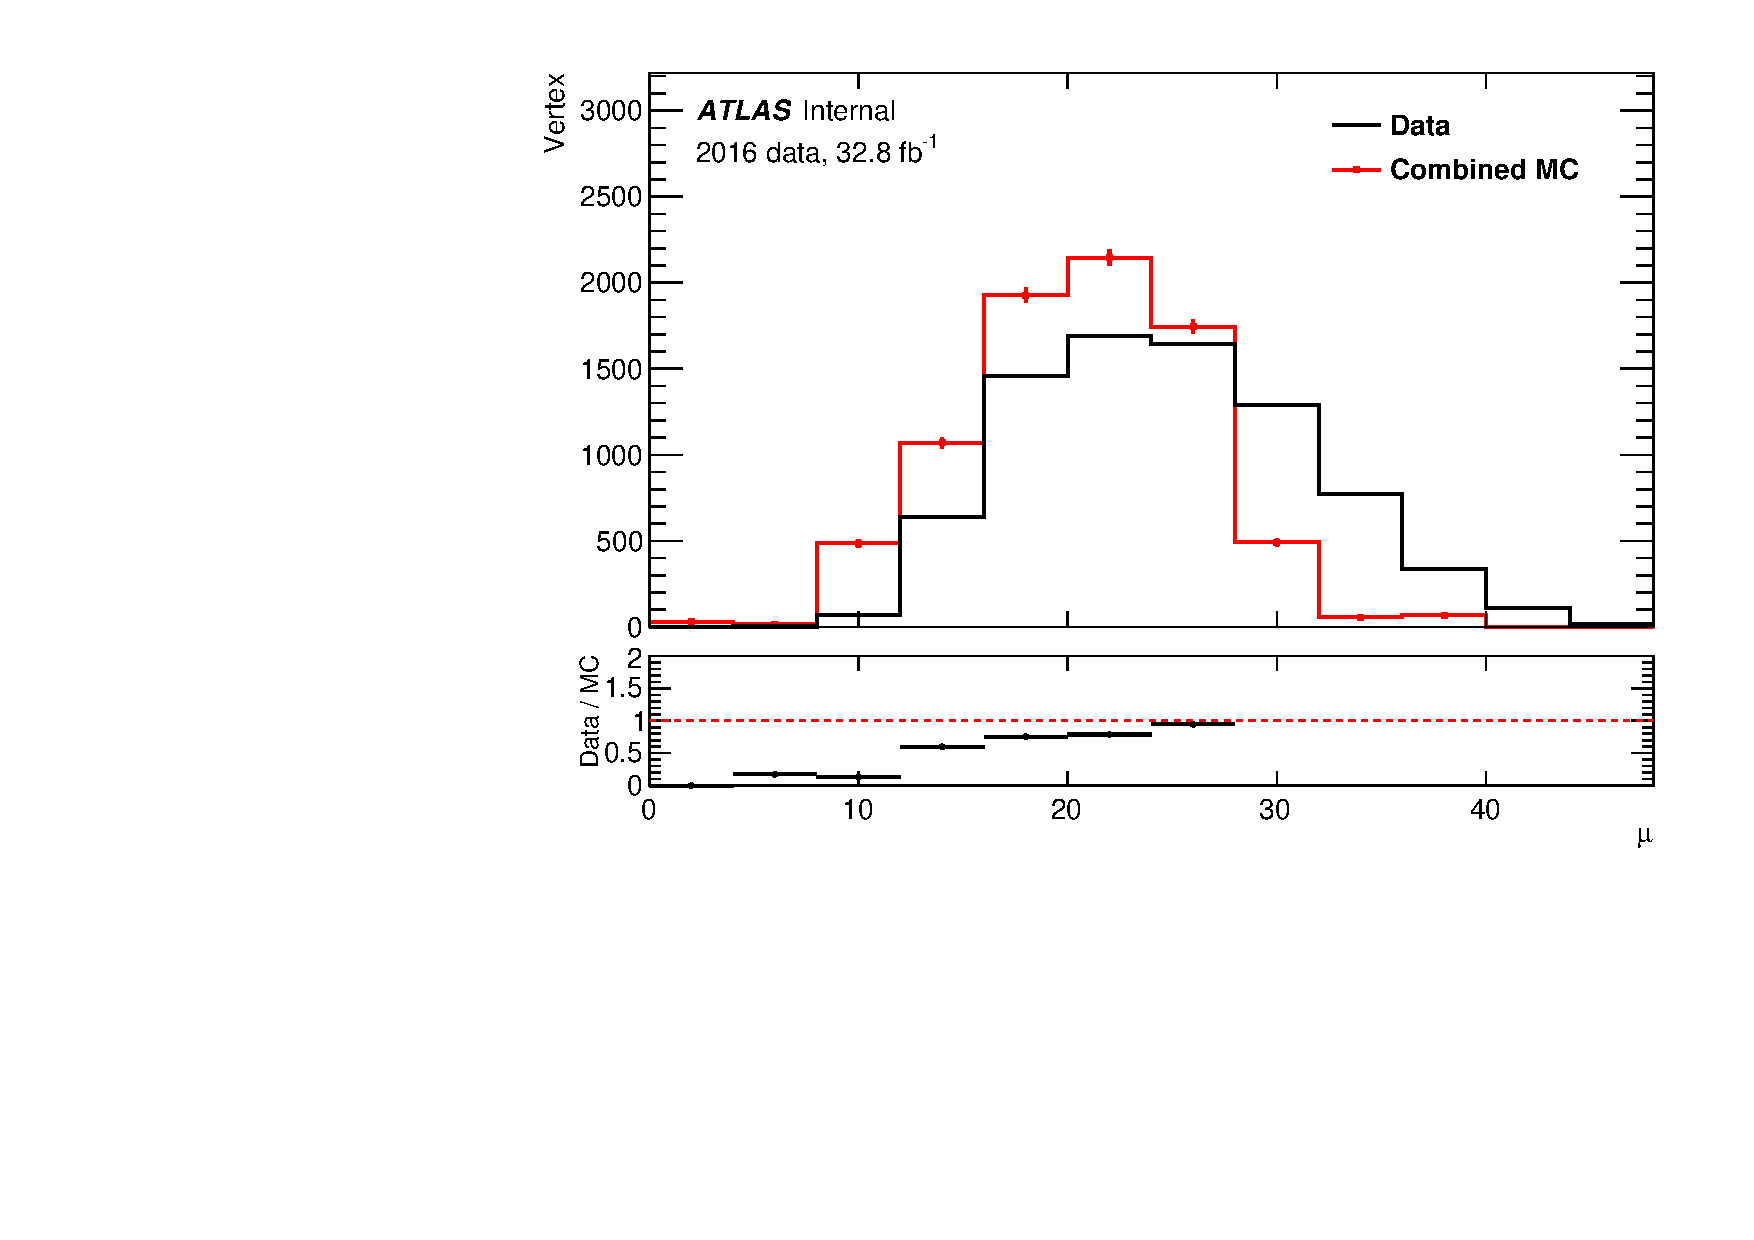
\includegraphics[width=0.45\textwidth]{figures/m_syst_Ks_mu.pdf}}
    \subfloat[]{\label{subfig:Ks_r}\includegraphics[width=0.45\textwidth]{figures/m_syst_Ks_r.pdf}}  \\
    \subfloat[]{\label{subfig:Ks_z}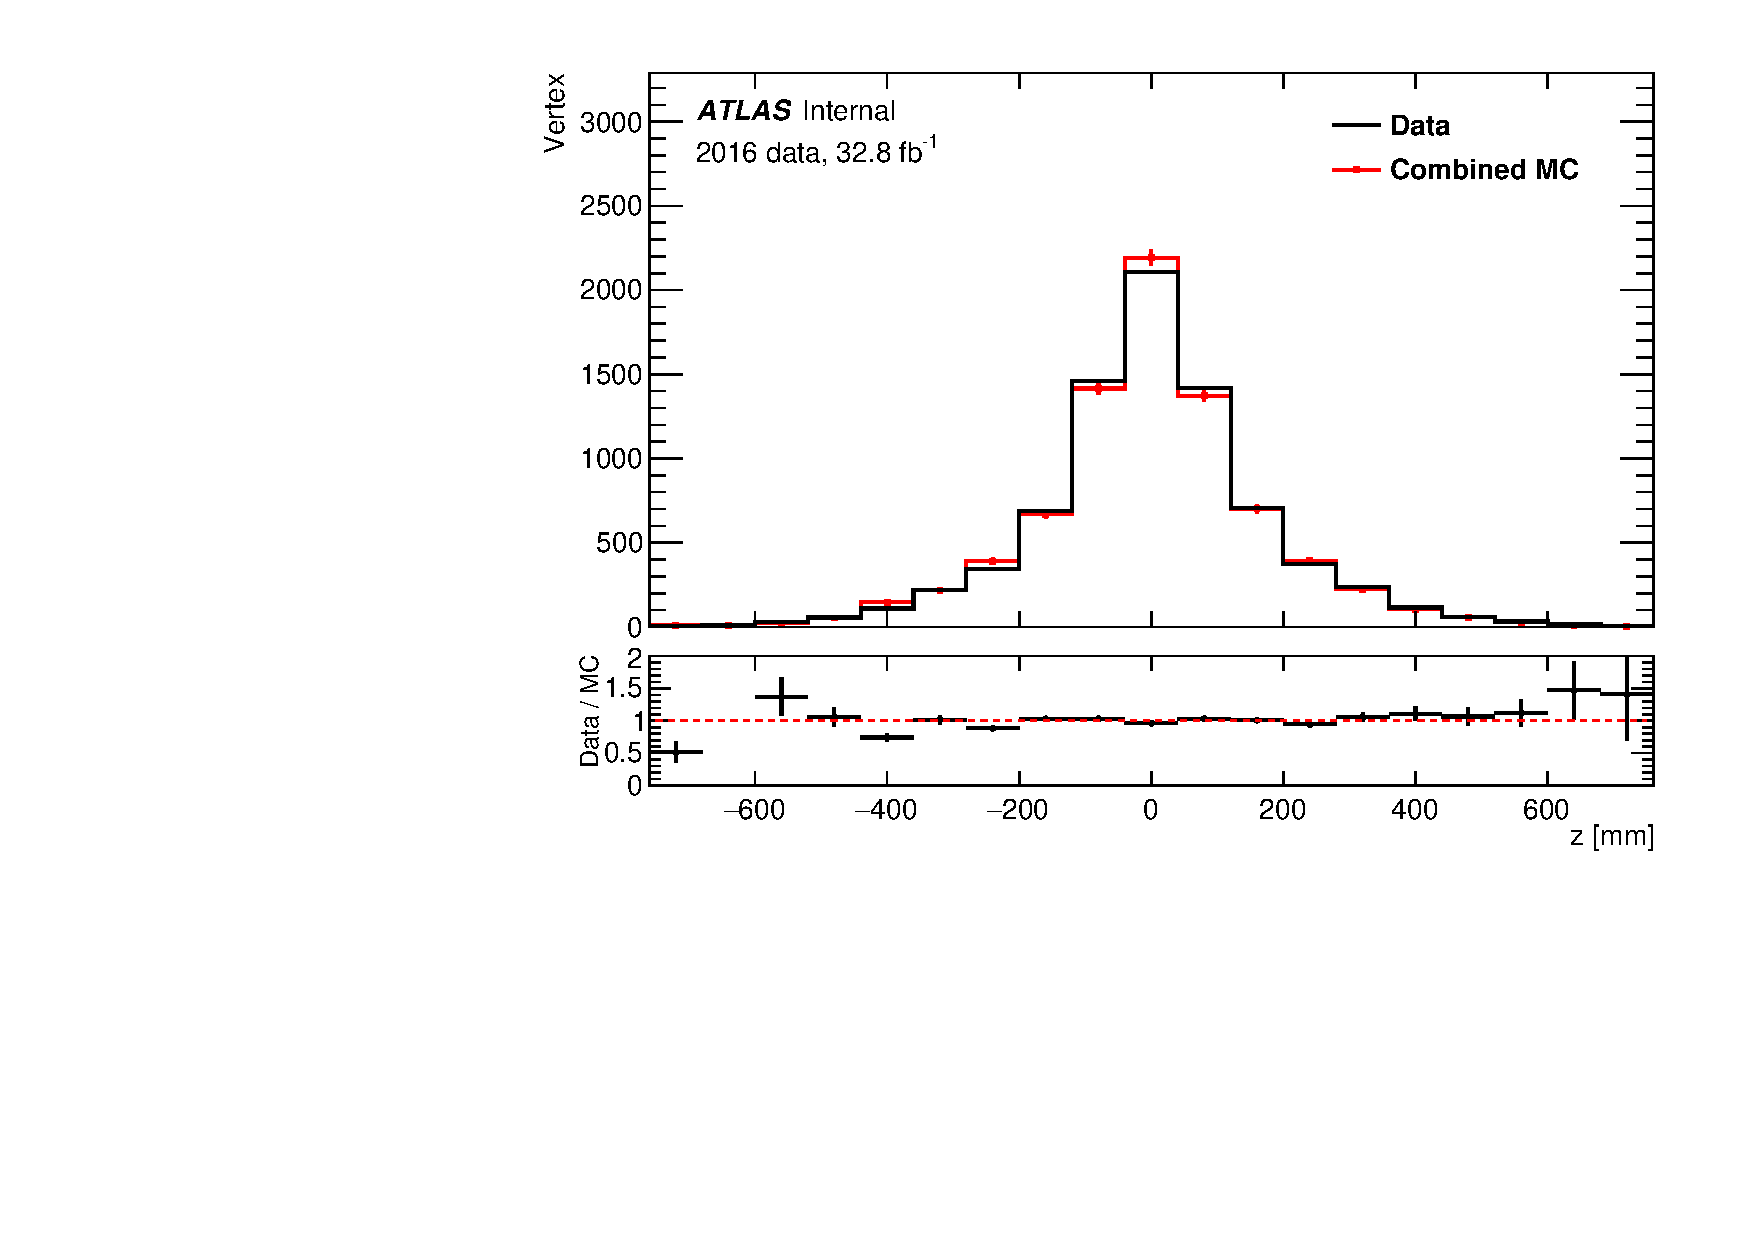
\includegraphics[width=0.45\textwidth]{figures/m_syst_Ks_z.pdf}} 
    \subfloat[]{\label{subfig:Ks_l}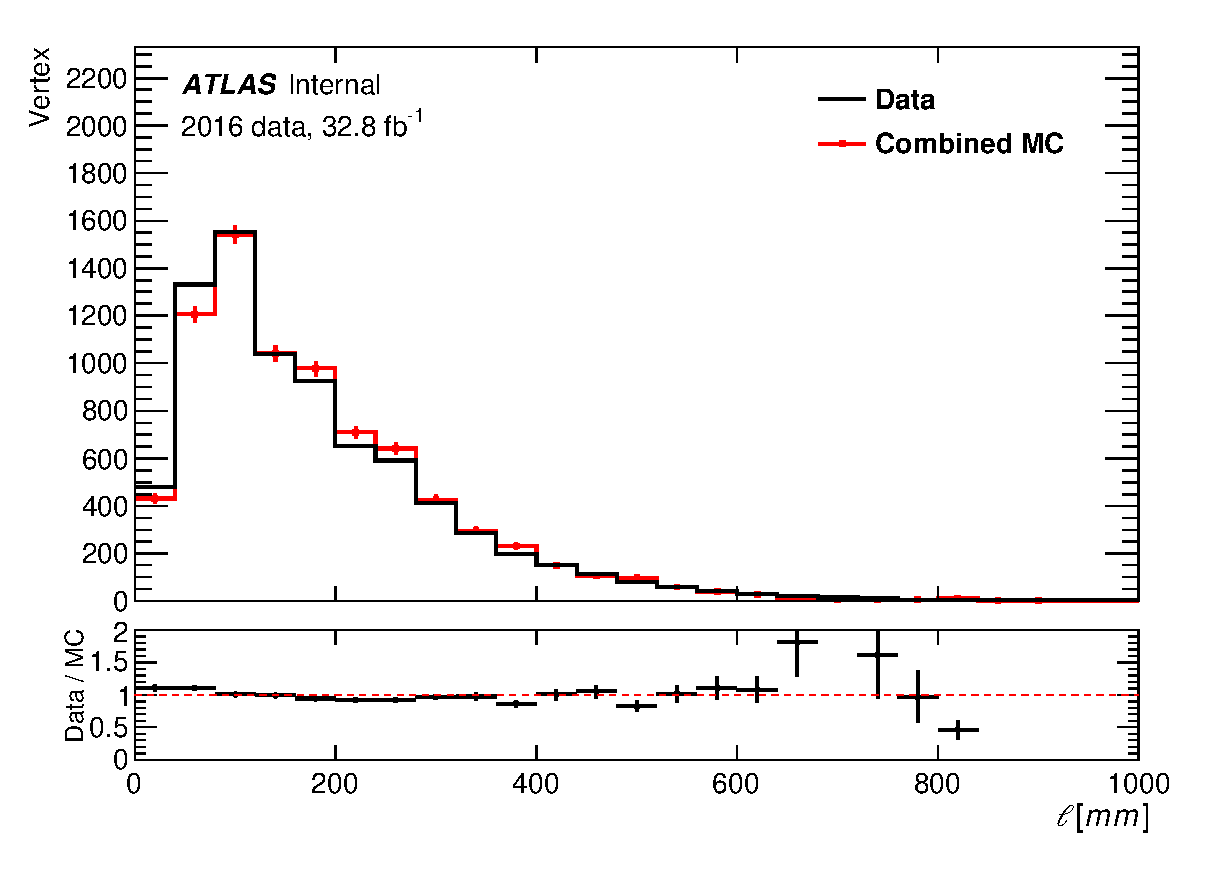
\includegraphics[width=0.45\textwidth]{figures/m_syst_Ks_l.eps}} \\
    \caption{Comparison of the (a) invariant mass, (b) $p_{T}$, (c) $\mu$, (d) transverse, (e) longitudinal position, and (f) decay length of $K_{S}$ in the data with the MC samples. Data is normalized to MC. In (d), the red dashed lines indicate the four Pixel layers and the first layer of SCT. The green dotted lines indicate the Inner Support Tube (45.5 mm) and Pixel Support Tube (229 mm).}
    \label{fig:Ks_data_MC}
\end{figure}

$K_{S}$ vertices found in the data and MC samples are binned in decay radius, $r$, and the $K_{S}$ yields in each bin are estimated from a fit using Breit-wigner. Figure~\ref{fig:Ks_fit} shows a few representative $K_{S}$ mass distributions (others are included in Appendix~\ref{app:syst_Ks_fit}). Background is negligible and hence not included in the fit. The estimated $K_{S}$ yields are normalized to the number of $K_{S}$ found in the lowest $r$ bin since the expected number of $K_{S}$ in the data samples is unknown. 

%\begin{figure}[tb]
\begin{figure}[!htb]
    \centering
    \subfloat[]{\label{subfig:Ks_fit_MC_1}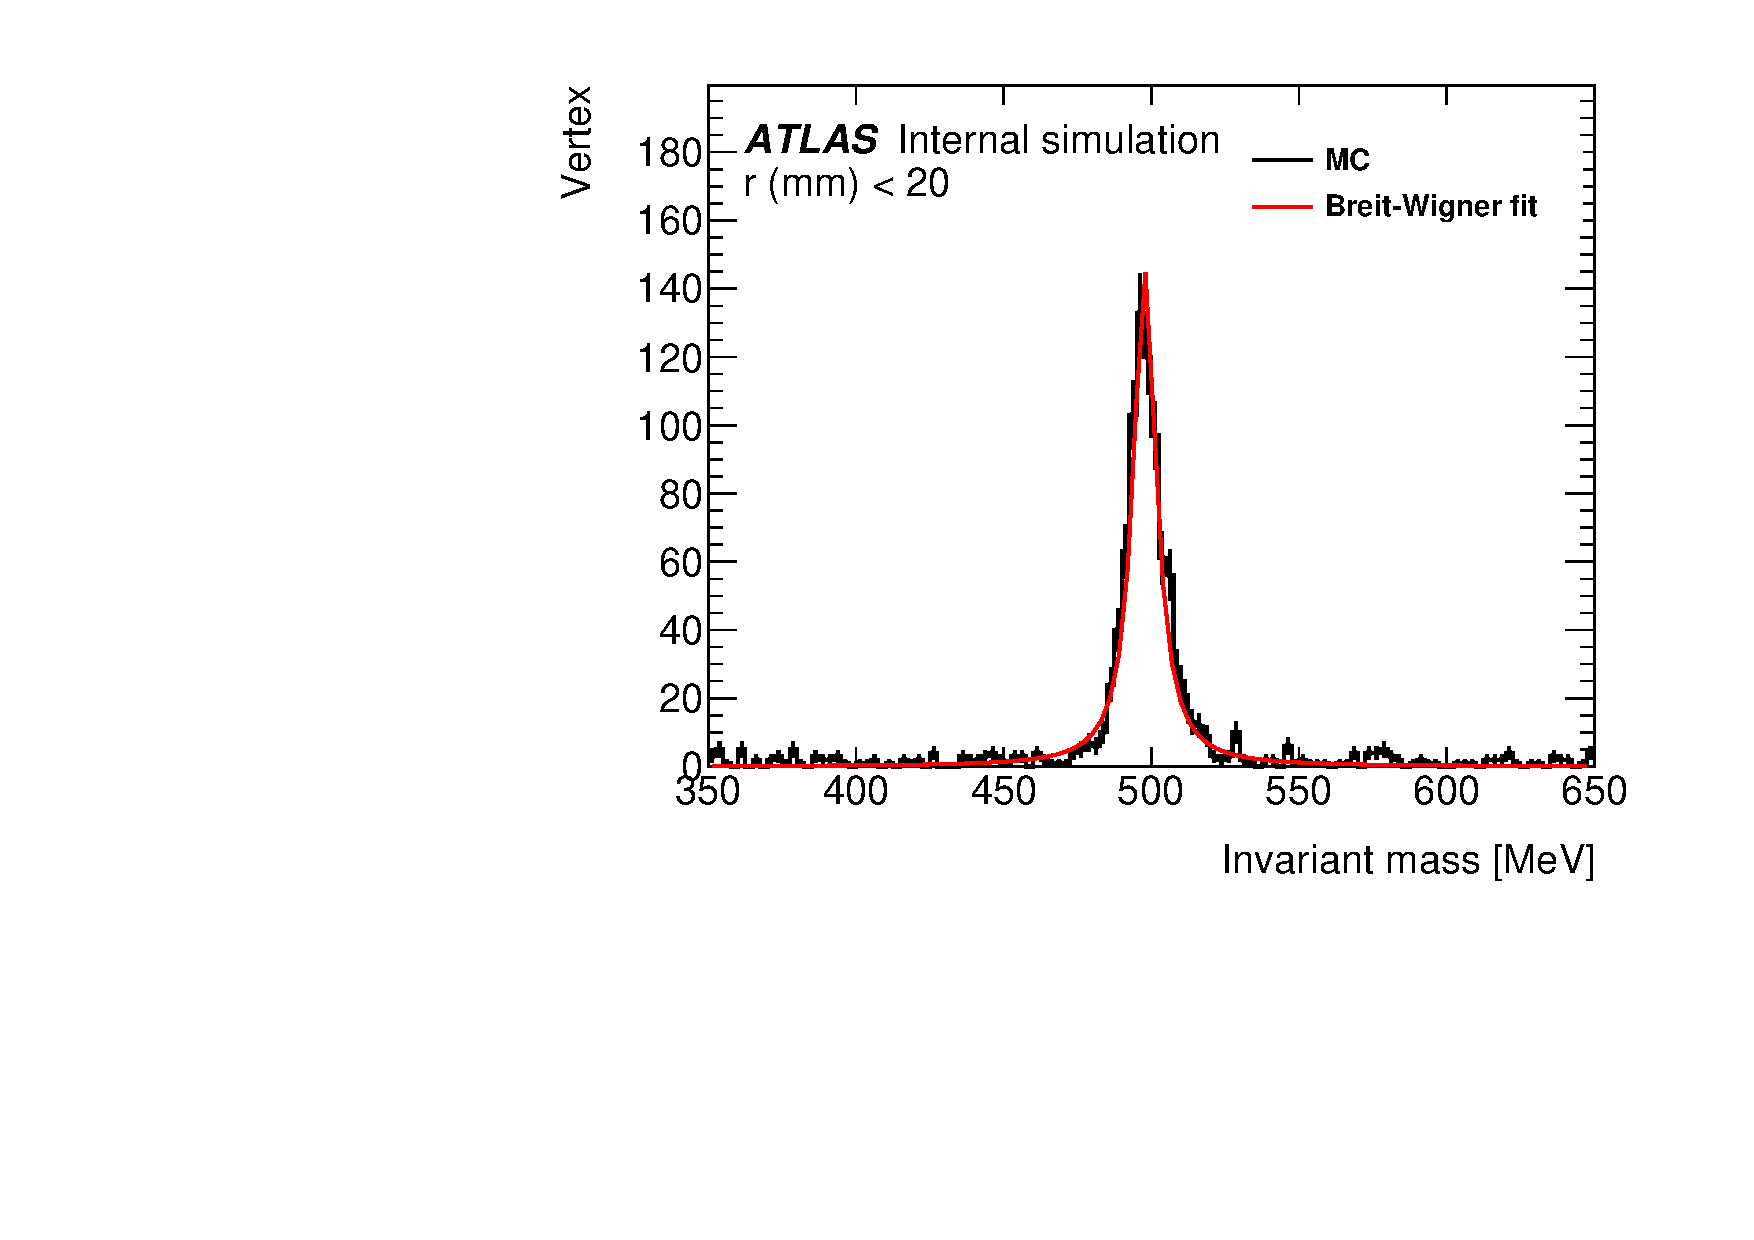
\includegraphics[width=0.45\textwidth]{figures/m_syst_Ks_Combined_MC_1}}
    \subfloat[]{\label{subfig:Ks_fit_MC_2}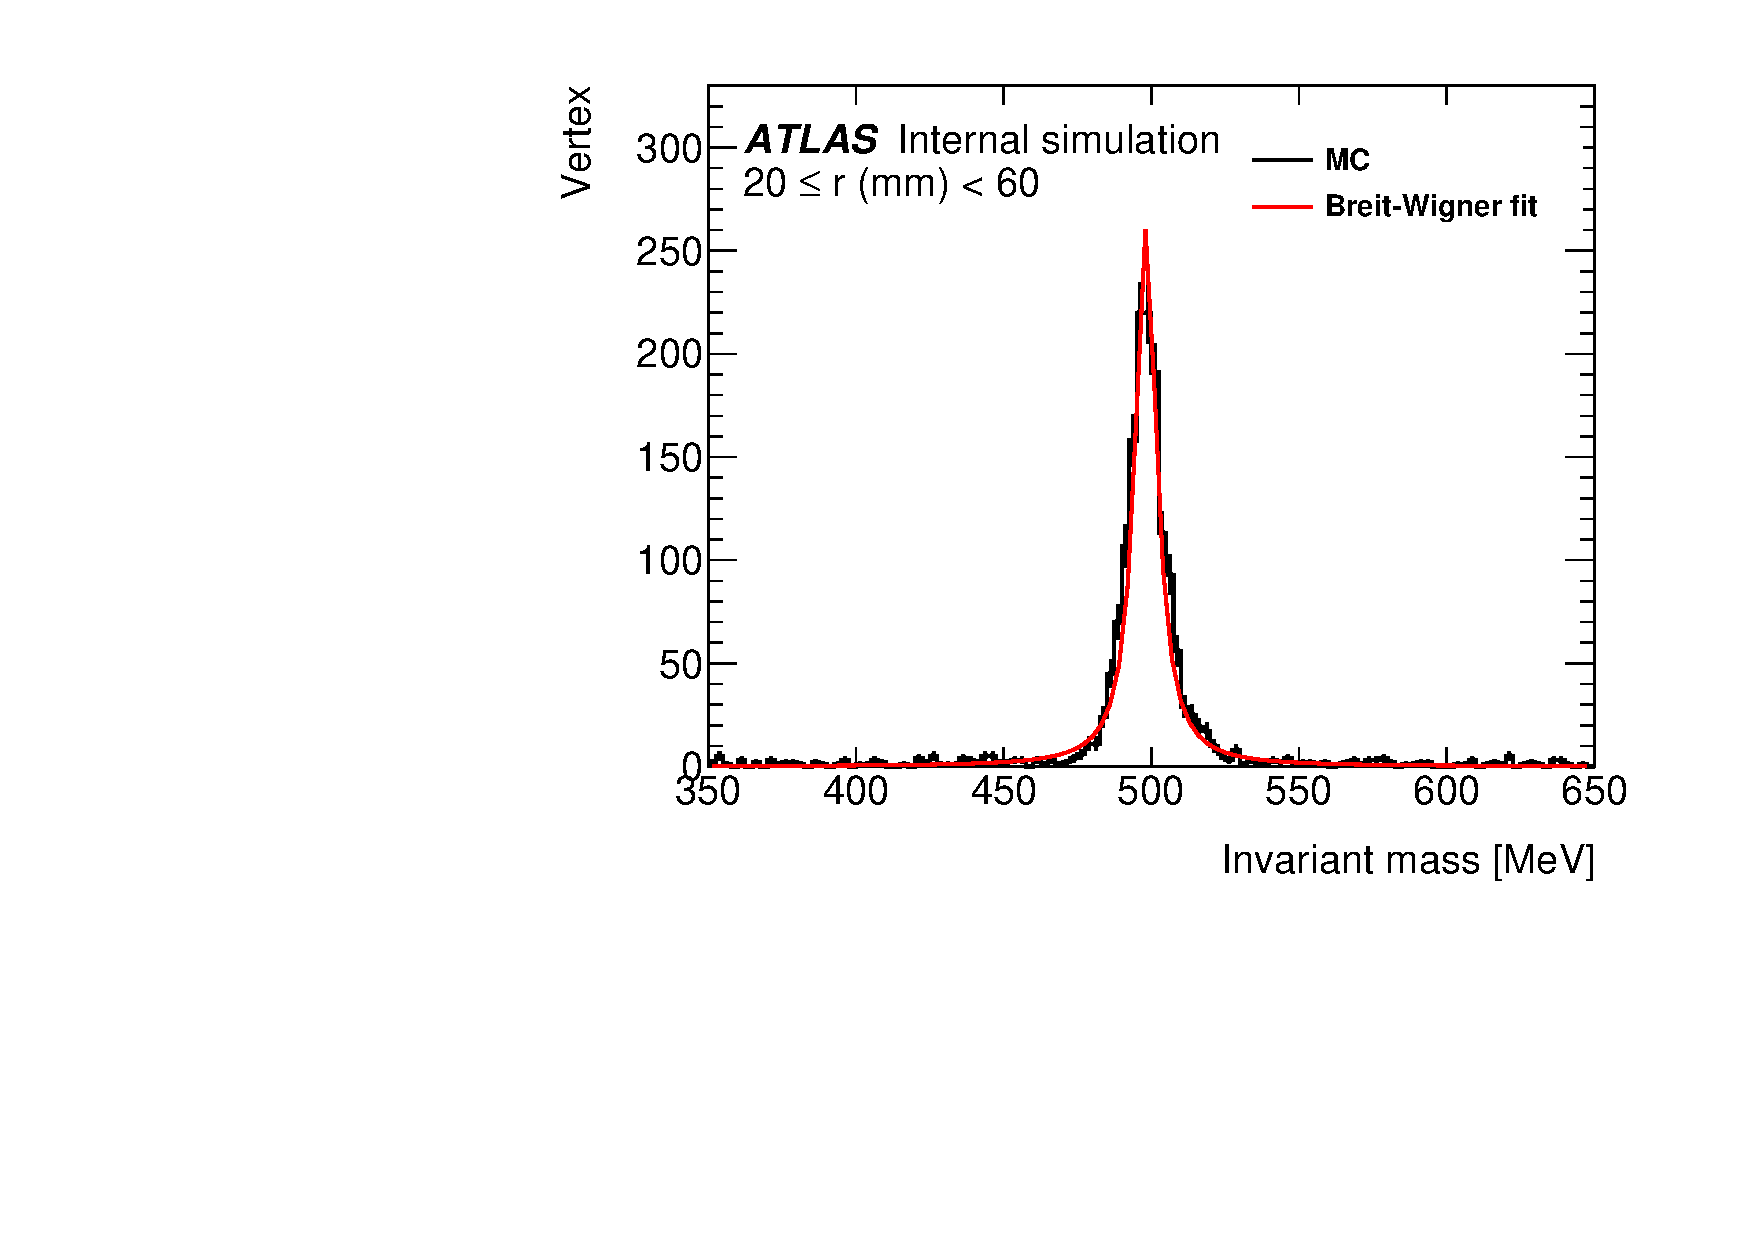
\includegraphics[width=0.45\textwidth]{figures/m_syst_Ks_Combined_MC_2}} \\
    \subfloat[]{\label{subfig:Ks_fit_Data_1}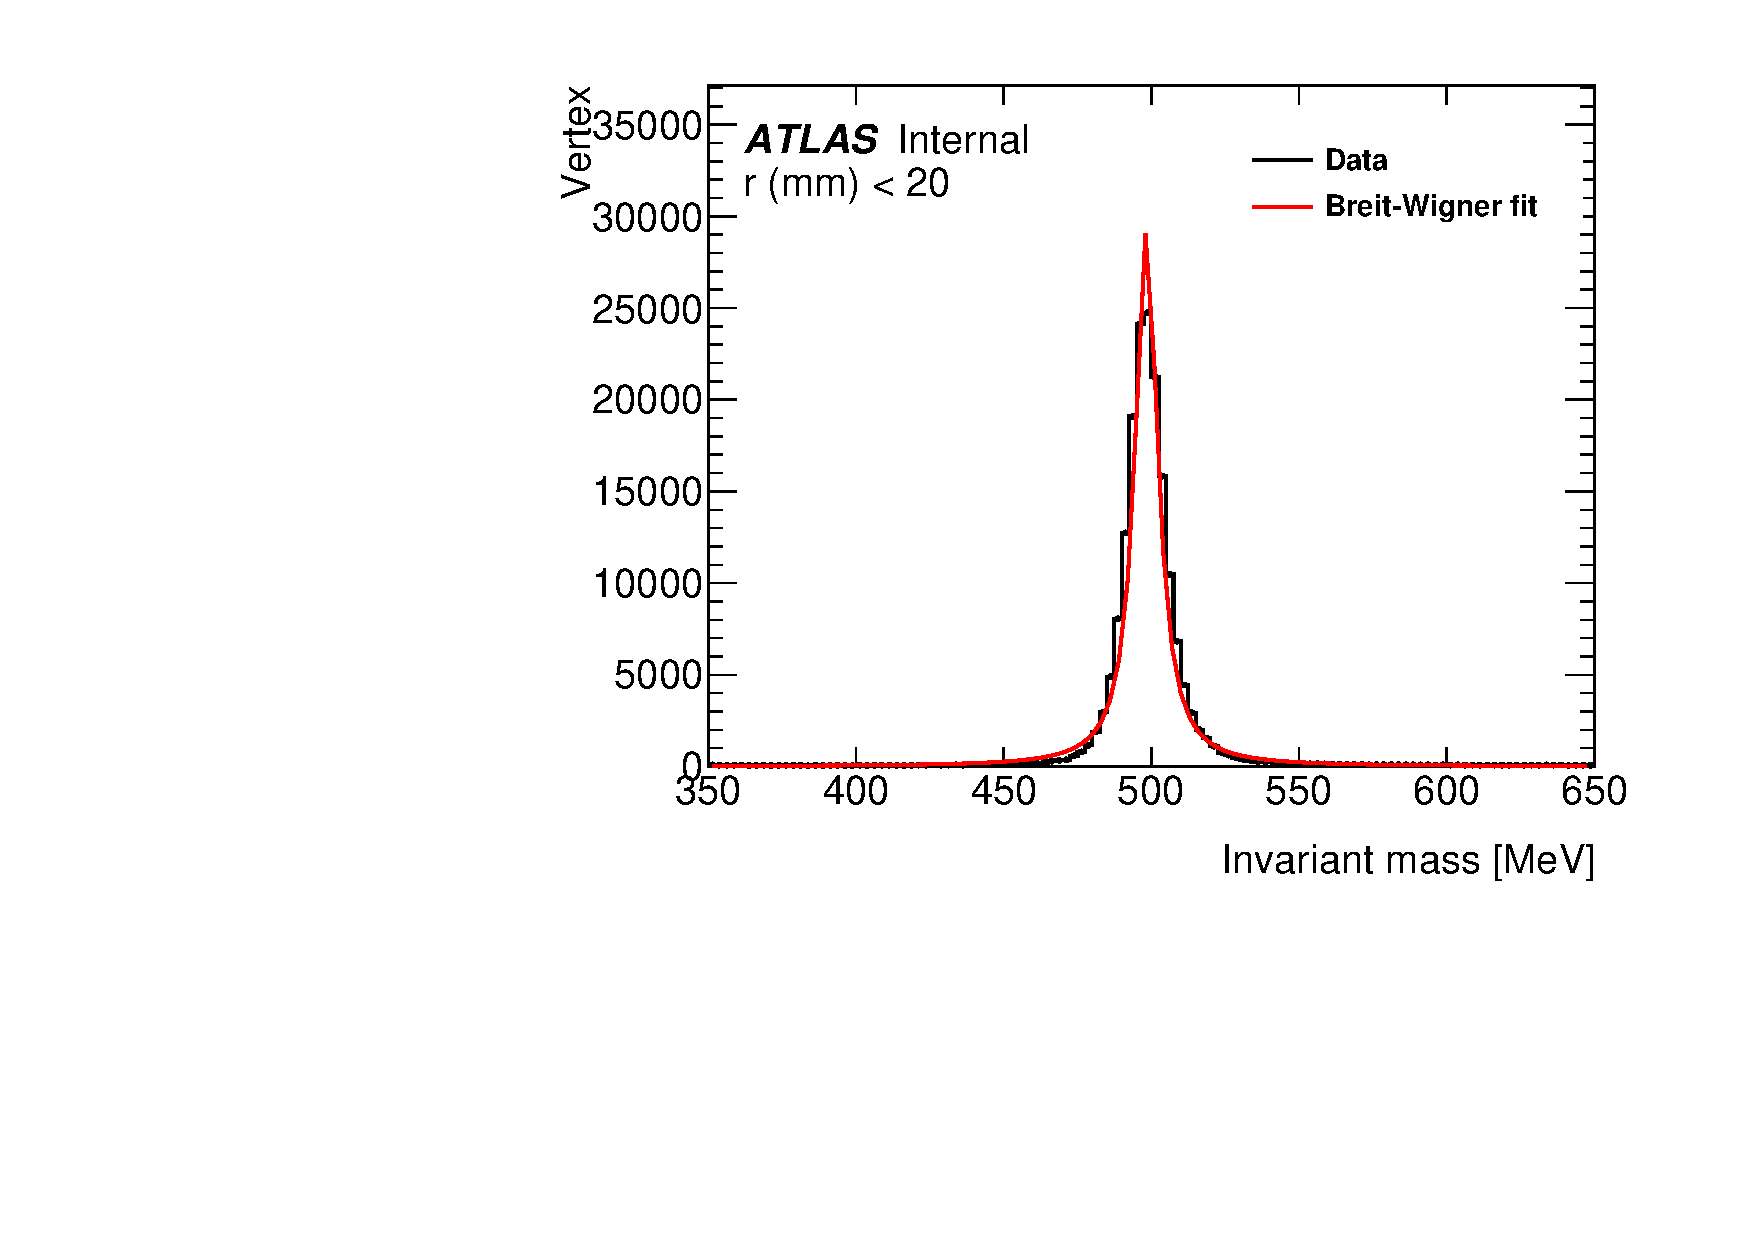
\includegraphics[width=0.45\textwidth]{figures/m_syst_Ks_Data_1}}
    \subfloat[]{\label{subfig:Ks_fit_Data_2}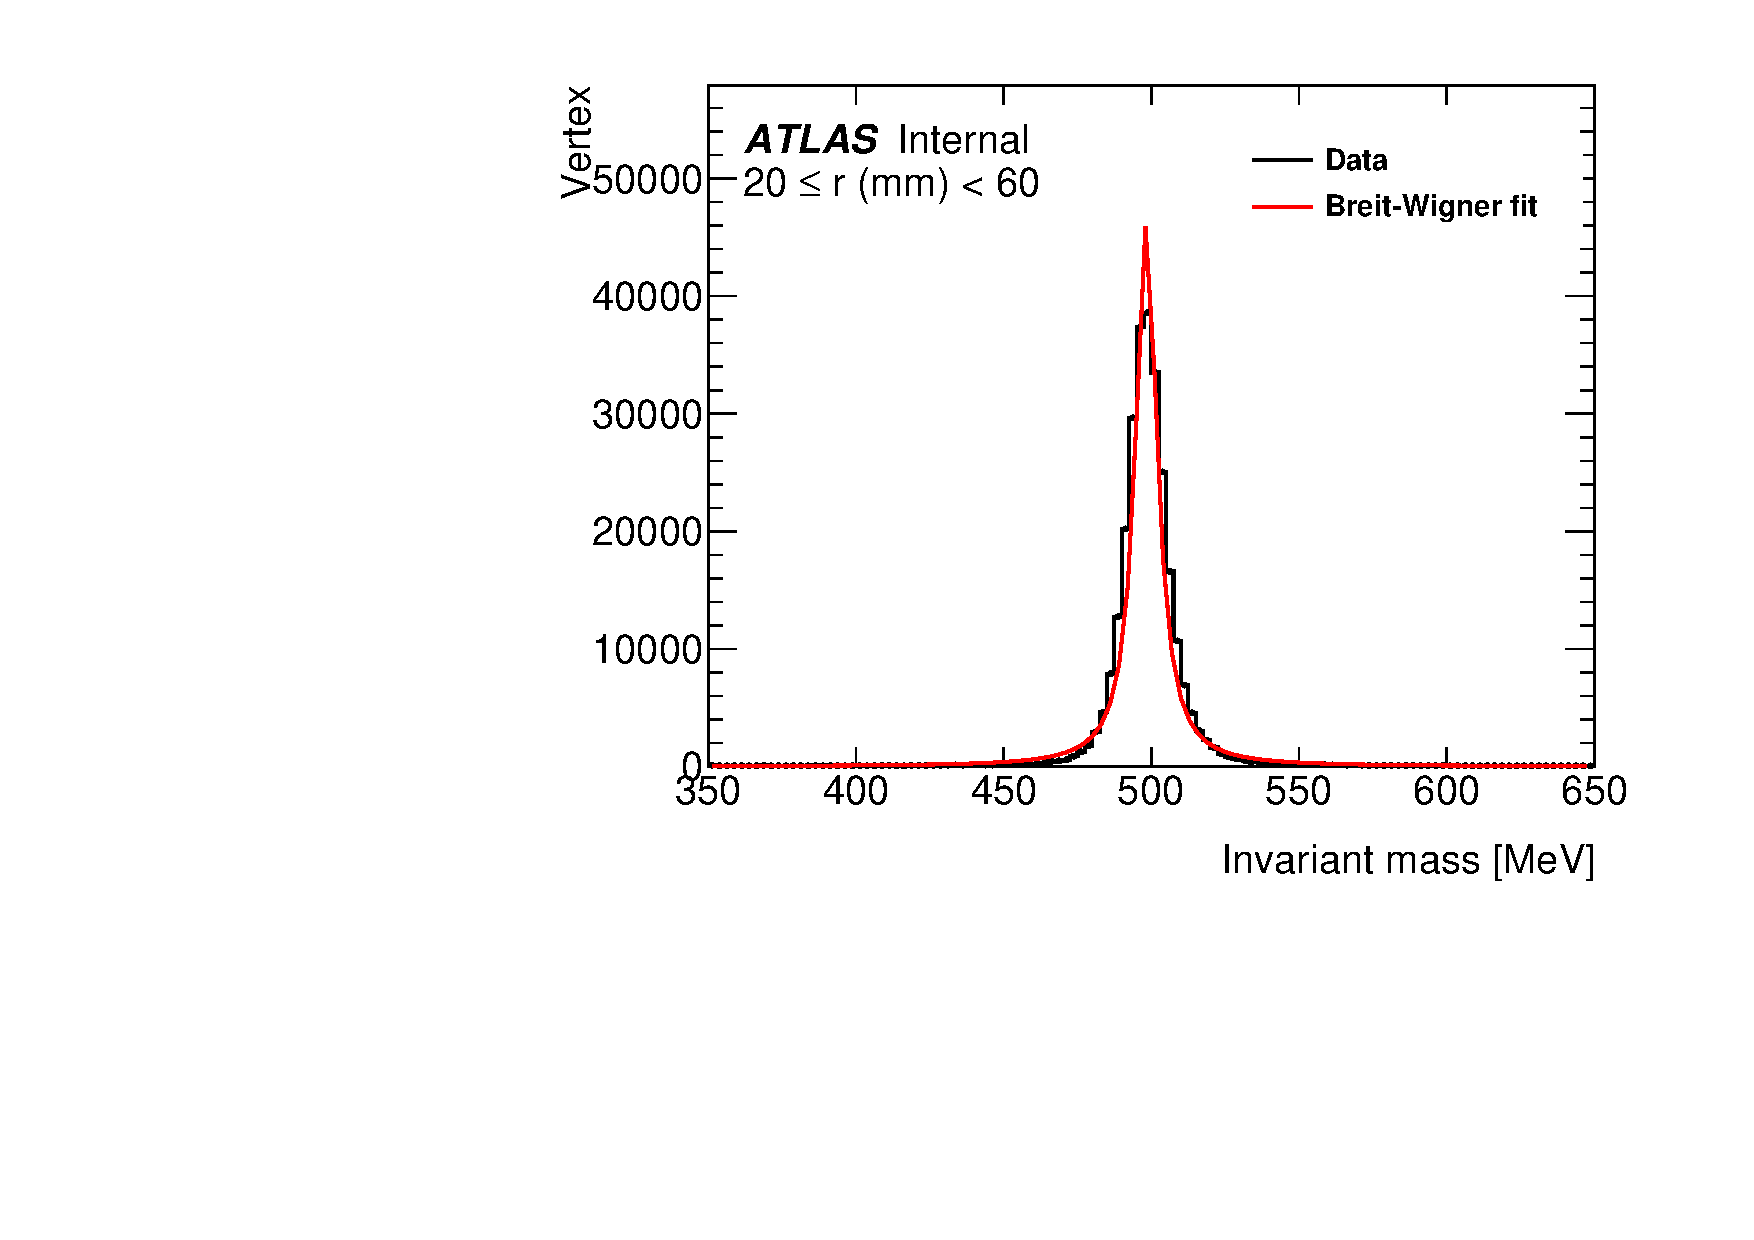
\includegraphics[width=0.45\textwidth]{figures/m_syst_Ks_Data_2}}
    \caption{Representative distributions of the $K_{S}$ invariant mass for (a) $r$ < 20 mm, and (b) 20 $<r<$ 60 mm in the background MC sample. The corresponding plots from the data sample are shown in (c) and (d). The mass distributions are fitted with a Breit-Wigner.}
    \label{fig:Ks_fit}
\end{figure}

%The systematic uncertainty in the lowest bin is taken from the run 2 study \cite{Aad:2011hd}. 
%The ratio of $K_{S}$ vertex yields in each bin of $r$ to $K_{S}$ vertex yields in the lowest $r$ bin is compared between the data and the background MC samples in Figure~\ref{fig:Ks_double_ratio}.
The $K_{S}$ yield, normalized to the yield with $r <$ 20 mm, is compared to the MC in Figure~\ref{fig:Ks_double_ratio}. The lower pane shows the double ratio,

\begin{equation}
\frac{N^{\mathrm{data}}_{R}}{N^{\mathrm{data}}_{R_{0}}} \bigg/ \frac{N^{\mathrm{MC}}_{R}}{N^{\mathrm{MC}}_{R_{0}}}
\label{eq:ks_double_ratio}
\end{equation}

which shows deviation from unity with increase of $r$. The difference in yield is then convoluted with the $r$ distribution of $Z'$ to estimate the systematic uncertainty in tracking and vertexing.

\begin{figure}[!htb]
	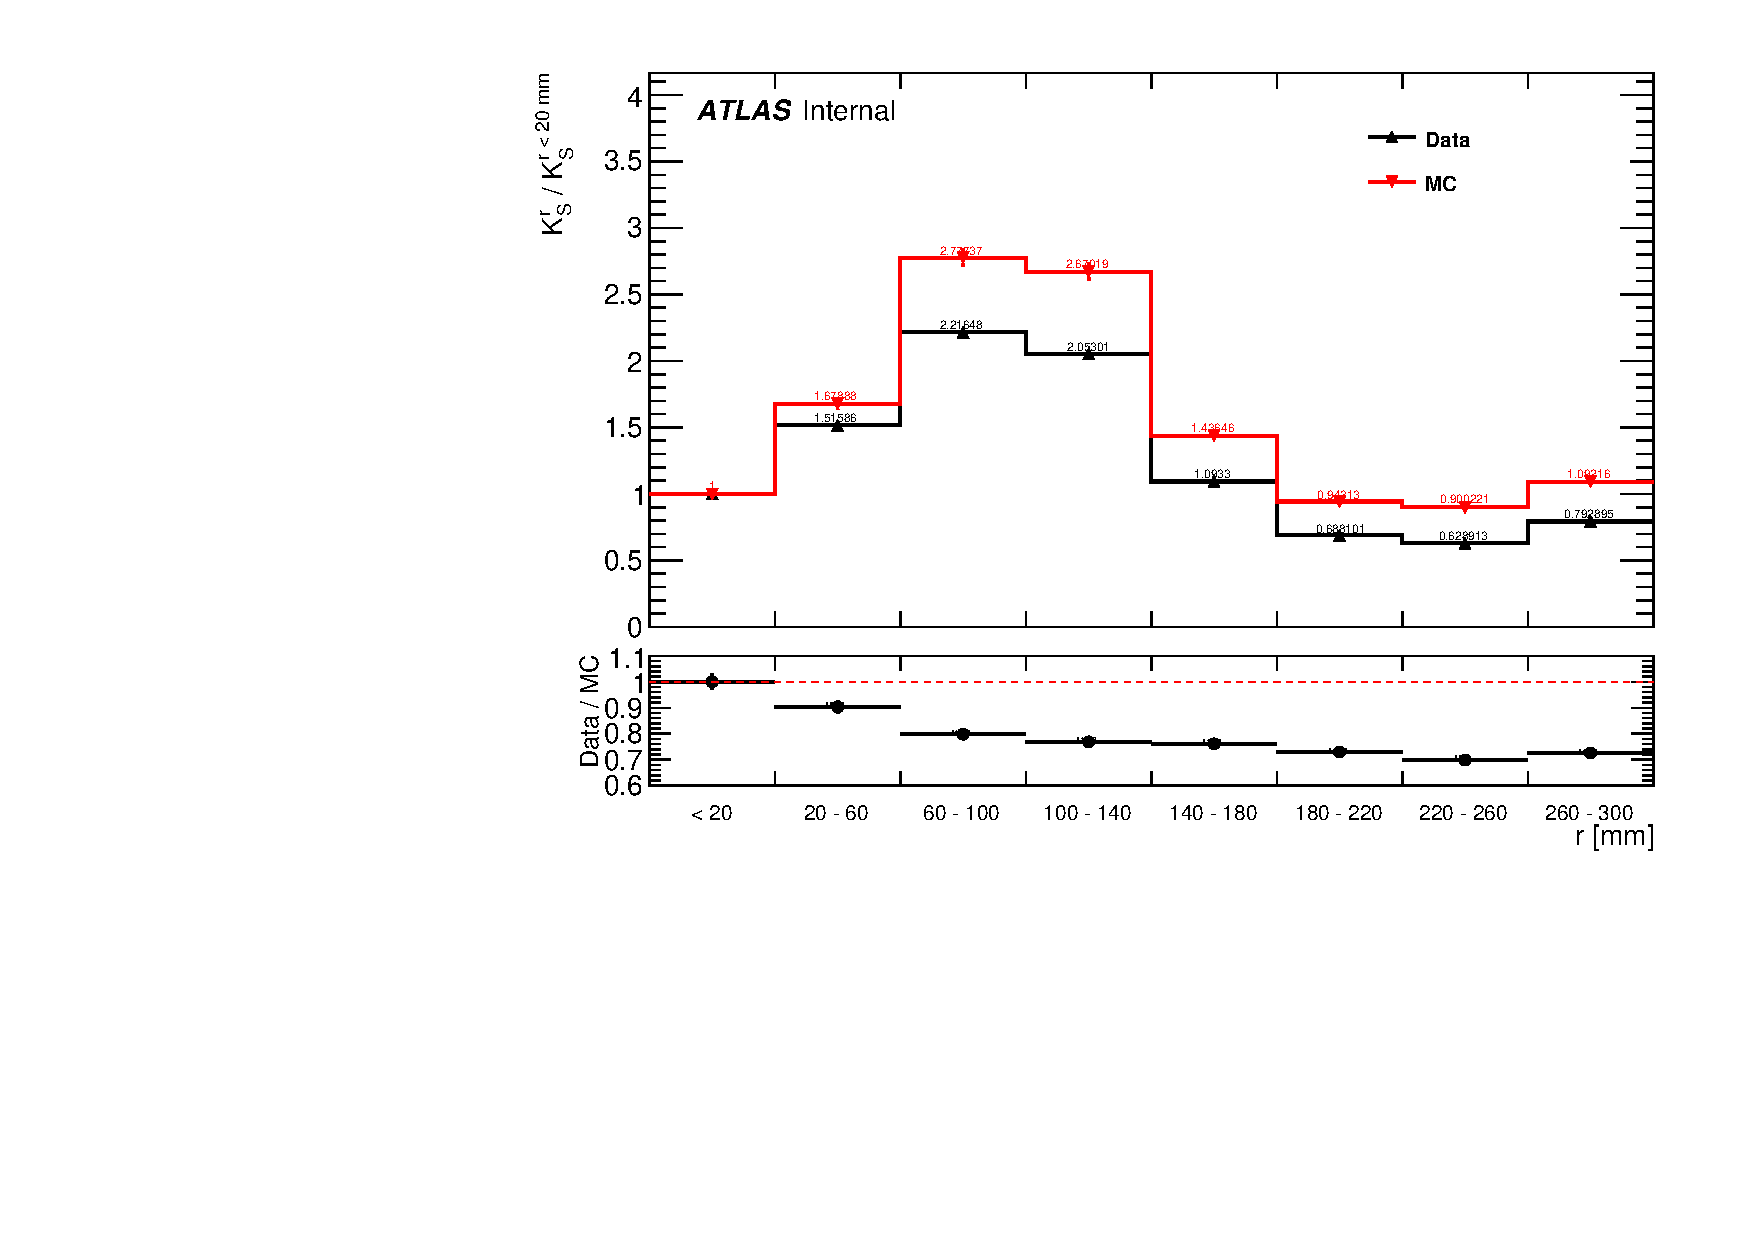
\includegraphics[width=0.50\textwidth]{figures/m_syst_Ks_ratio.pdf}
	\centering
	\caption{The radial distribution of $K_{S}$ yield, normalized to the lowest $r$ bin in the data and MC samples. The lower pane shows the double ratio as defined in the text.}
	\label{fig:Ks_double_ratio}
\end{figure}



\subsection{Systematic uncertainties on lepton identification}
\label{sec:syst_leptonID}

\subsection{Systematic uncertainties on trigger efficiency}
\label{sec:syst_trigger}


%-------------------------------------------------------------------------------
\section{Results}
\label{sec:result}
%-------------------------------------------------------------------------------



% All figures and tables should appear before the summary and conclusion.
% The package placeins provides the macro \FloatBarrier to achieve this.
\FloatBarrier
%-------------------------------------------------------------------------------
\section{Conclusion}
\label{sec:conclusion}
%-------------------------------------------------------------------------------


%-------------------------------------------------------------------------------
% If you use biblatex and either biber or bibtex to process the bibliography
% just say \printbibliography here
\newpage
\printbibliography
% If you want to use the traditional BibTeX you need to use the syntax below.
%\bibliographystyle{bib/bst/atlasBibStyleWithTitle}
%\bibliography{DispDilep-INT-2017,bib/ATLAS,bib/CMS,bib/ConfNotes,bib/PubNotes}
%-------------------------------------------------------------------------------

%-------------------------------------------------------------------------------
% Print the list of contributors to the analysis
% The argument gives the fraction of the text width used for the names
%-------------------------------------------------------------------------------
\clearpage
%The supporting notes for the analysis should also contain a list of contributors.
%This information should usually be included in \texttt{mydocument-metadata.tex}.
%The list should be printed either here or before the Table of Contents.
\PrintAtlasContribute{0.30}


%-------------------------------------------------------------------------------
\clearpage
\appendix
\part*{Appendices}
\addcontentsline{toc}{part}{Appendices}
%-------------------------------------------------------------------------------

\appendix
\section{Truth-level $p_{T}$ and $\eta$ distributions of Signal MC samples}
\label{app:signal_truth}
\input{sections/app_signal_truth.tex}

\newpage

\section{$K_{S}$ yields in data and MC samples used for tracking and vertexing systematic uncertainties}
\label{app:syst_Ks_fit}
%\begin{figure}[tb]
\begin{figure}[!htb]
    \centering
    \subfloat[MC, $60$ mm $<r<$ 100 mm]{\label{subfig:Ks_fit_MC_3}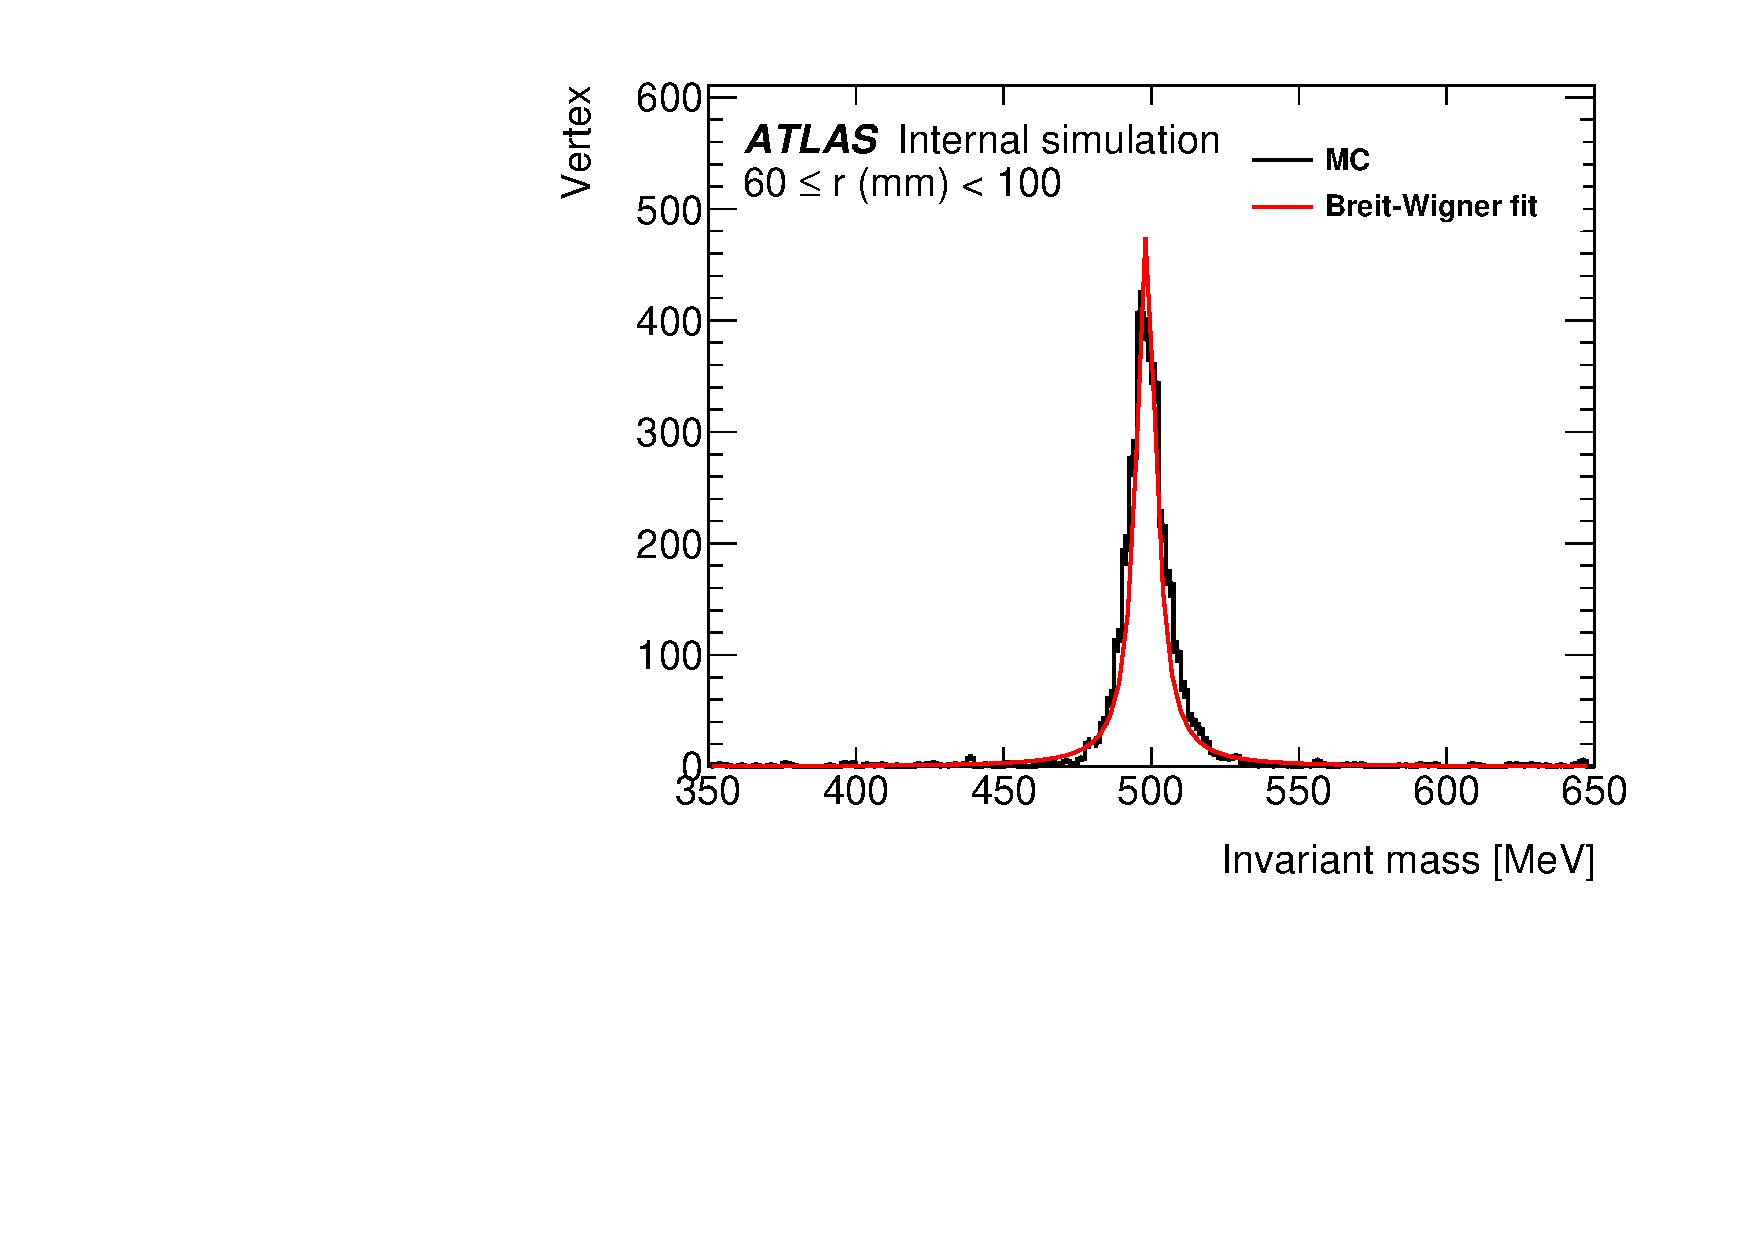
\includegraphics[width=0.33\textwidth]{figures/m_syst_Ks_Combined_MC_3}} 
    \subfloat[MC, $100$ mm $<r<$ 140 mm]{\label{subfig:Ks_fit_MC_4}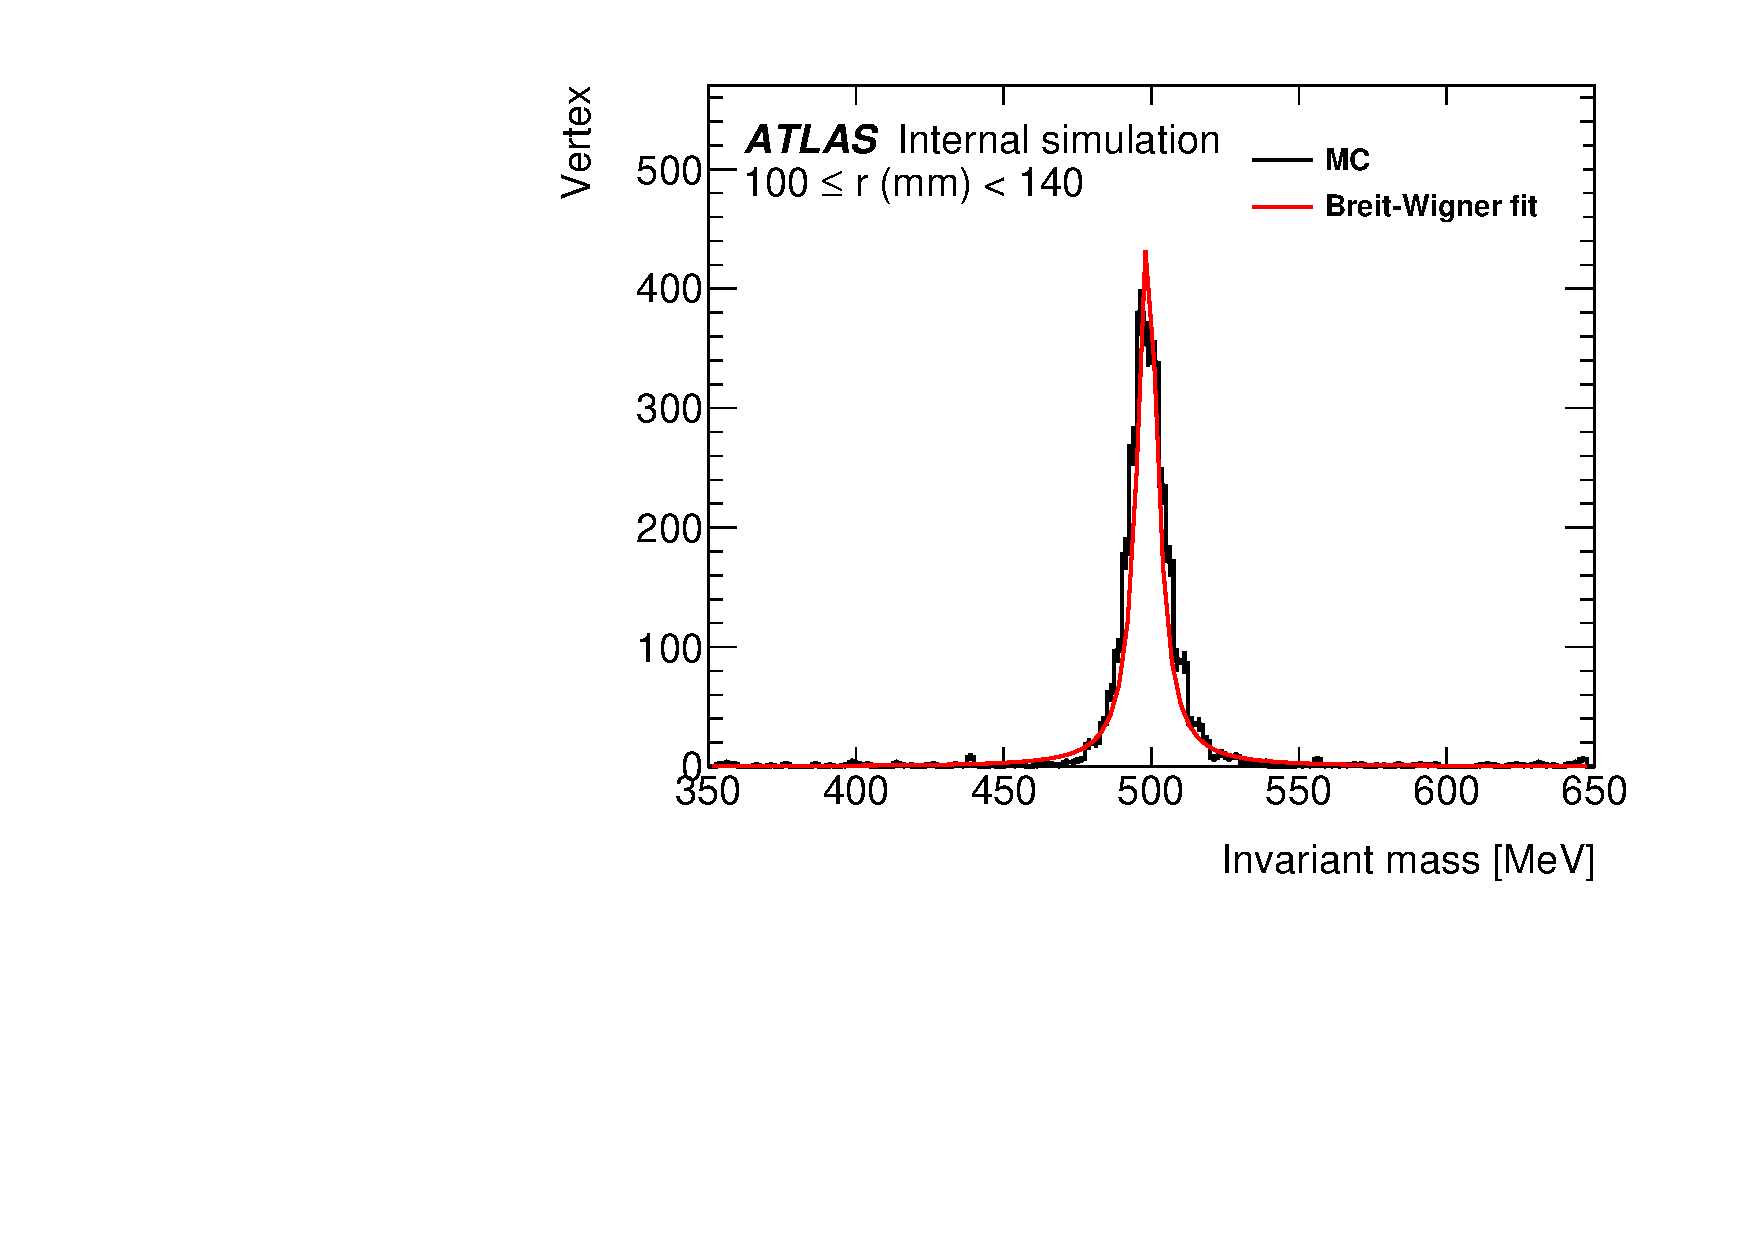
\includegraphics[width=0.33\textwidth]{figures/m_syst_Ks_Combined_MC_4}}
    \subfloat[MC, $140$ mm $<r<$ 180 mm]{\label{subfig:Ks_fit_MC_5}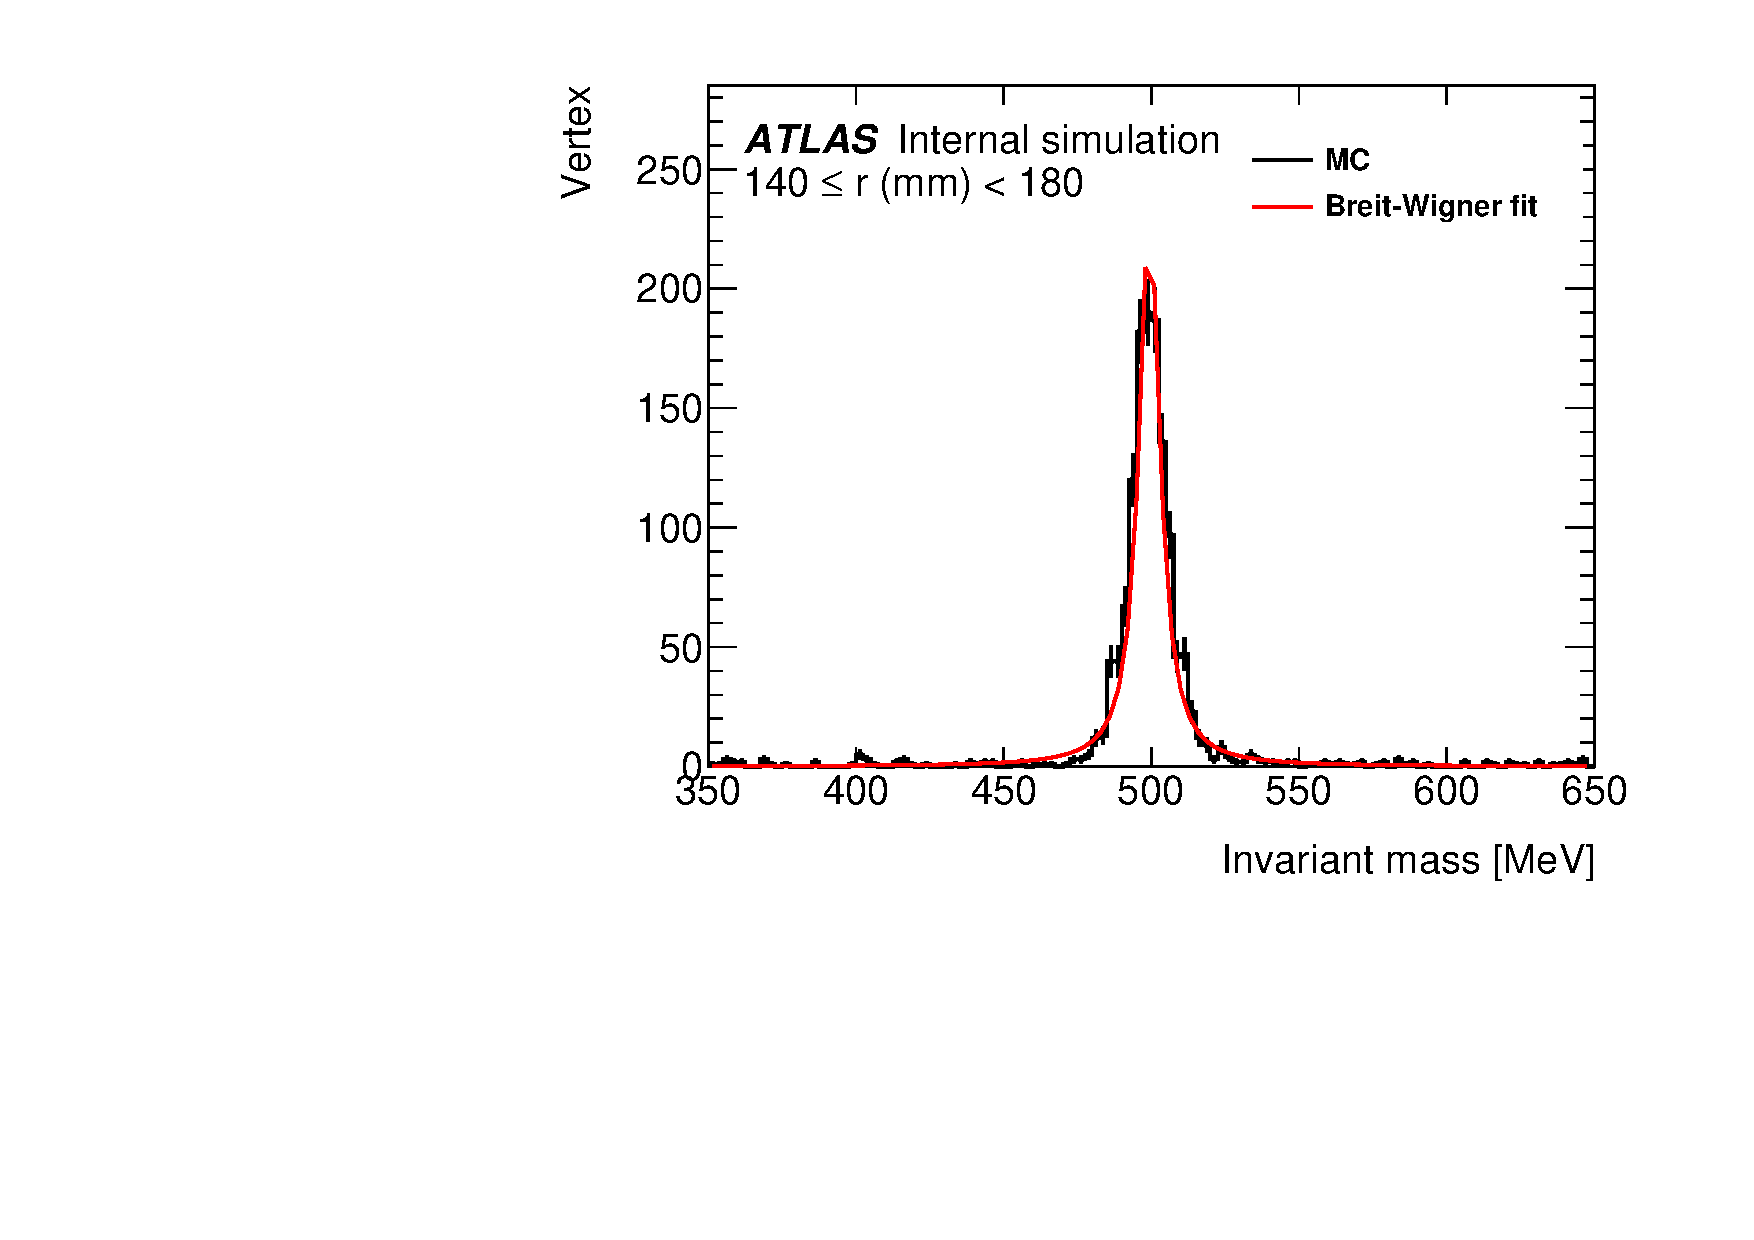
\includegraphics[width=0.33\textwidth]{figures/m_syst_Ks_Combined_MC_5}} \\
    \subfloat[MC, $180$ mm $<r<$ 220 mm]{\label{subfig:Ks_fit_MC_6}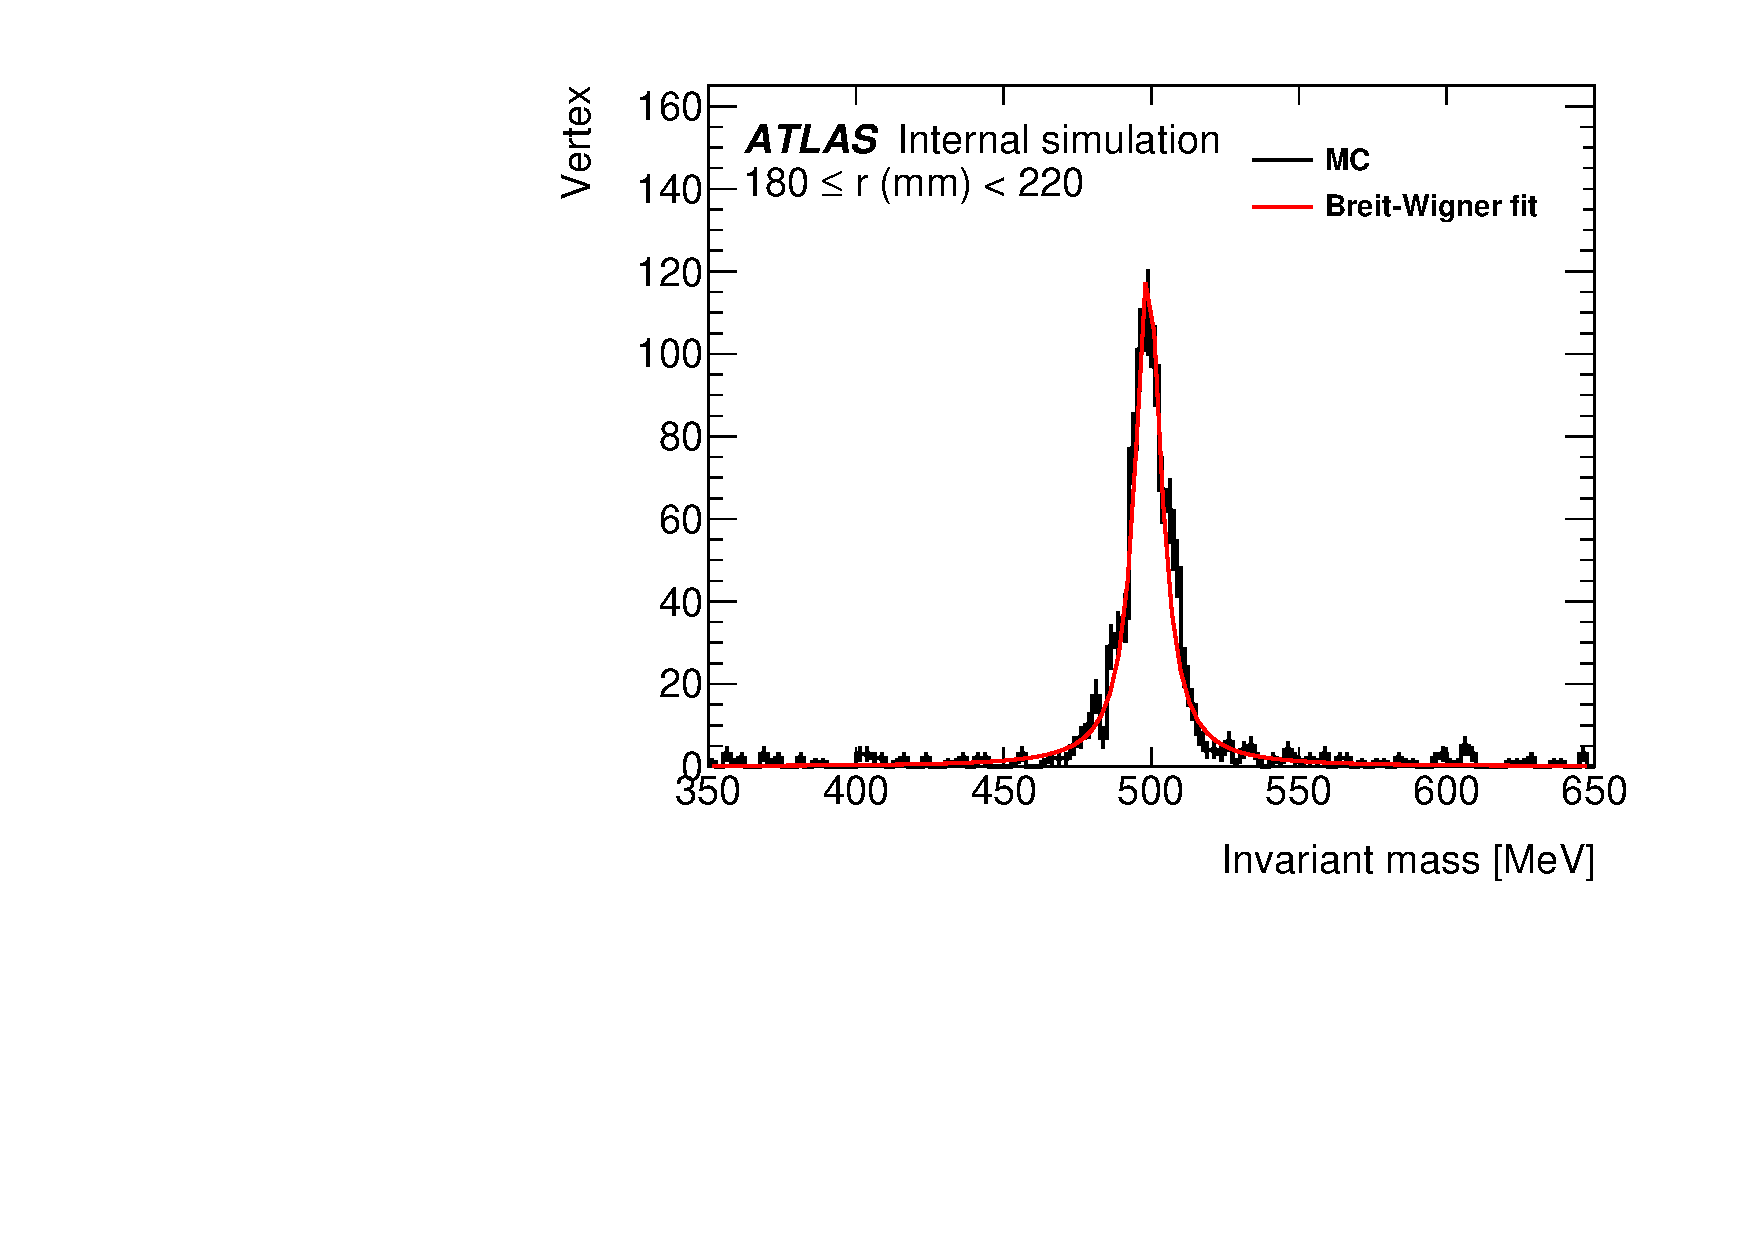
\includegraphics[width=0.33\textwidth]{figures/m_syst_Ks_Combined_MC_6}} 
    \subfloat[MC, $220$ mm $<r<$ 260 mm]{\label{subfig:Ks_fit_MC_7}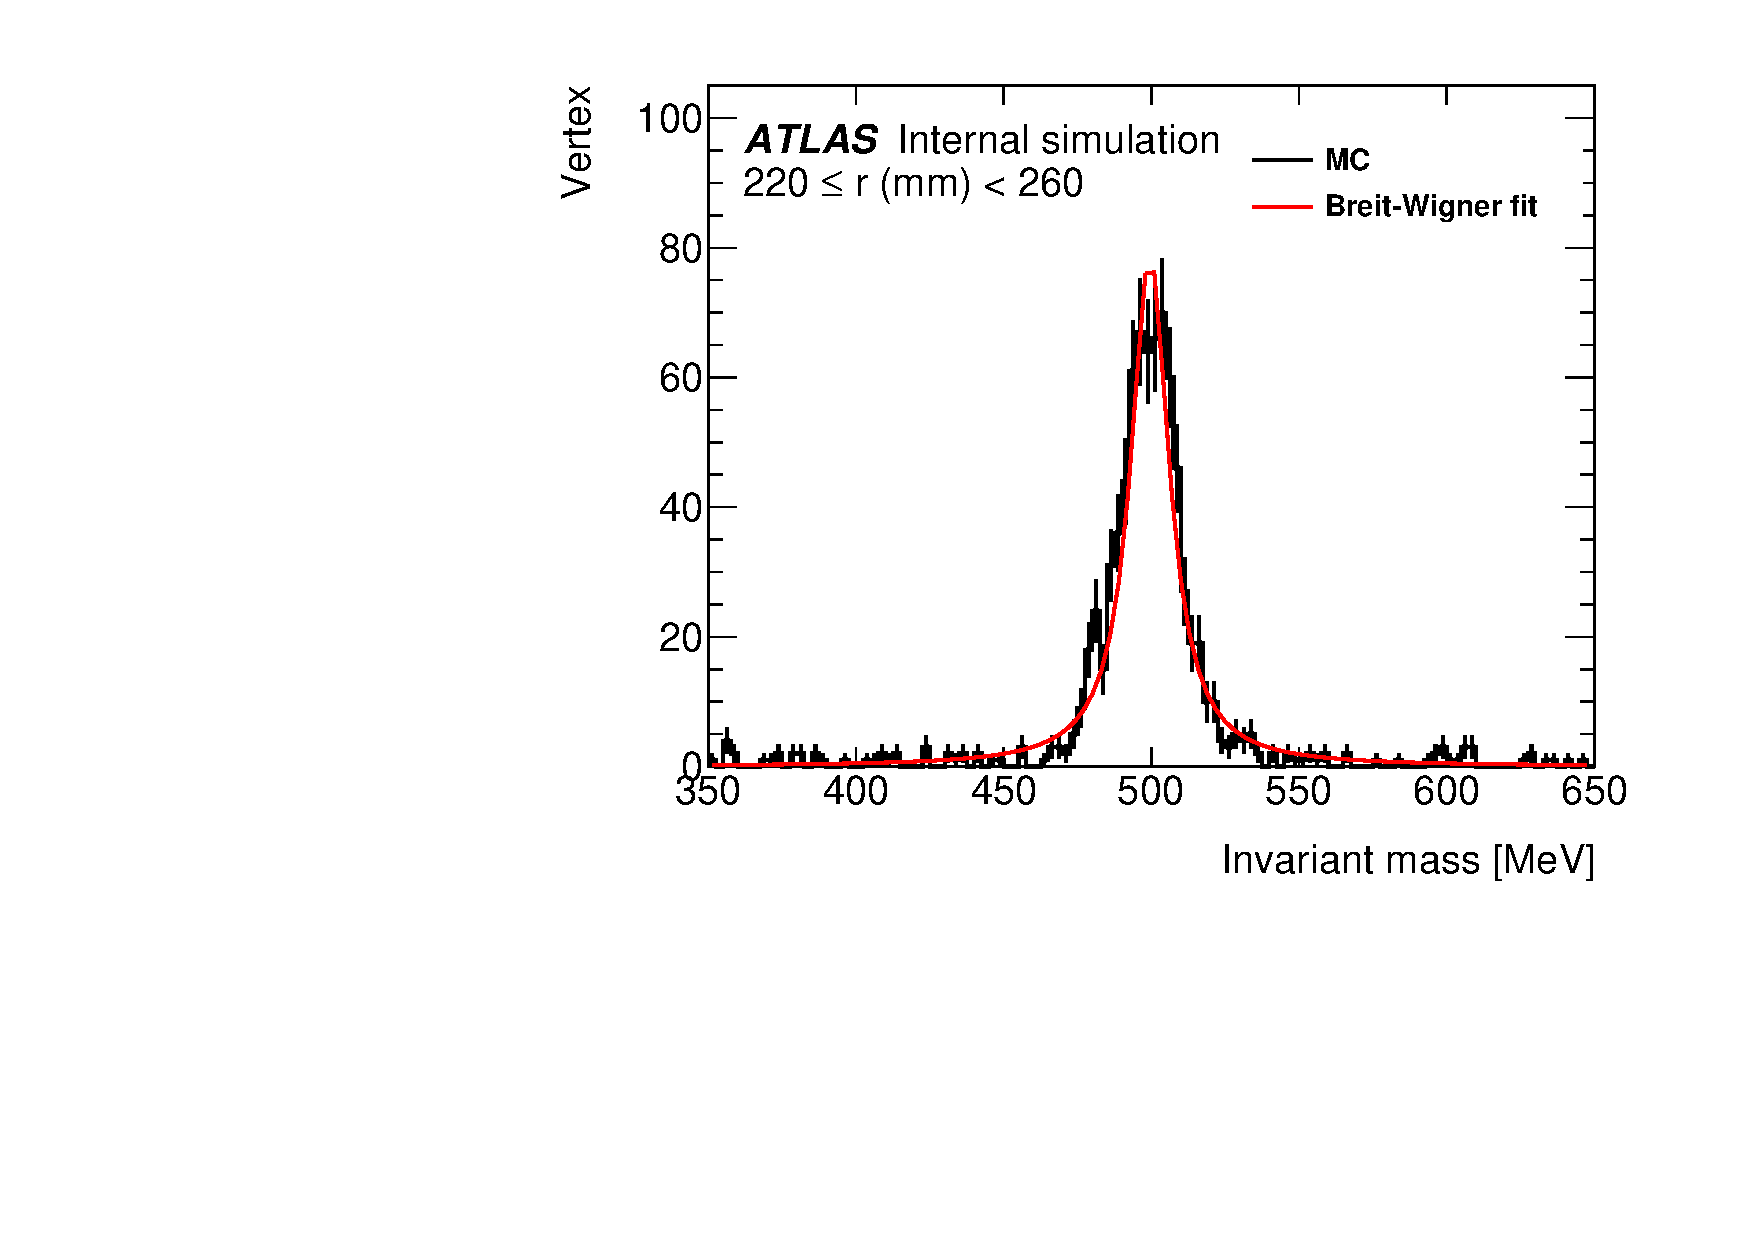
\includegraphics[width=0.33\textwidth]{figures/m_syst_Ks_Combined_MC_7}}
    \subfloat[MC, $260$ mm $<r<$ 300 mm]{\label{subfig:Ks_fit_MC_8}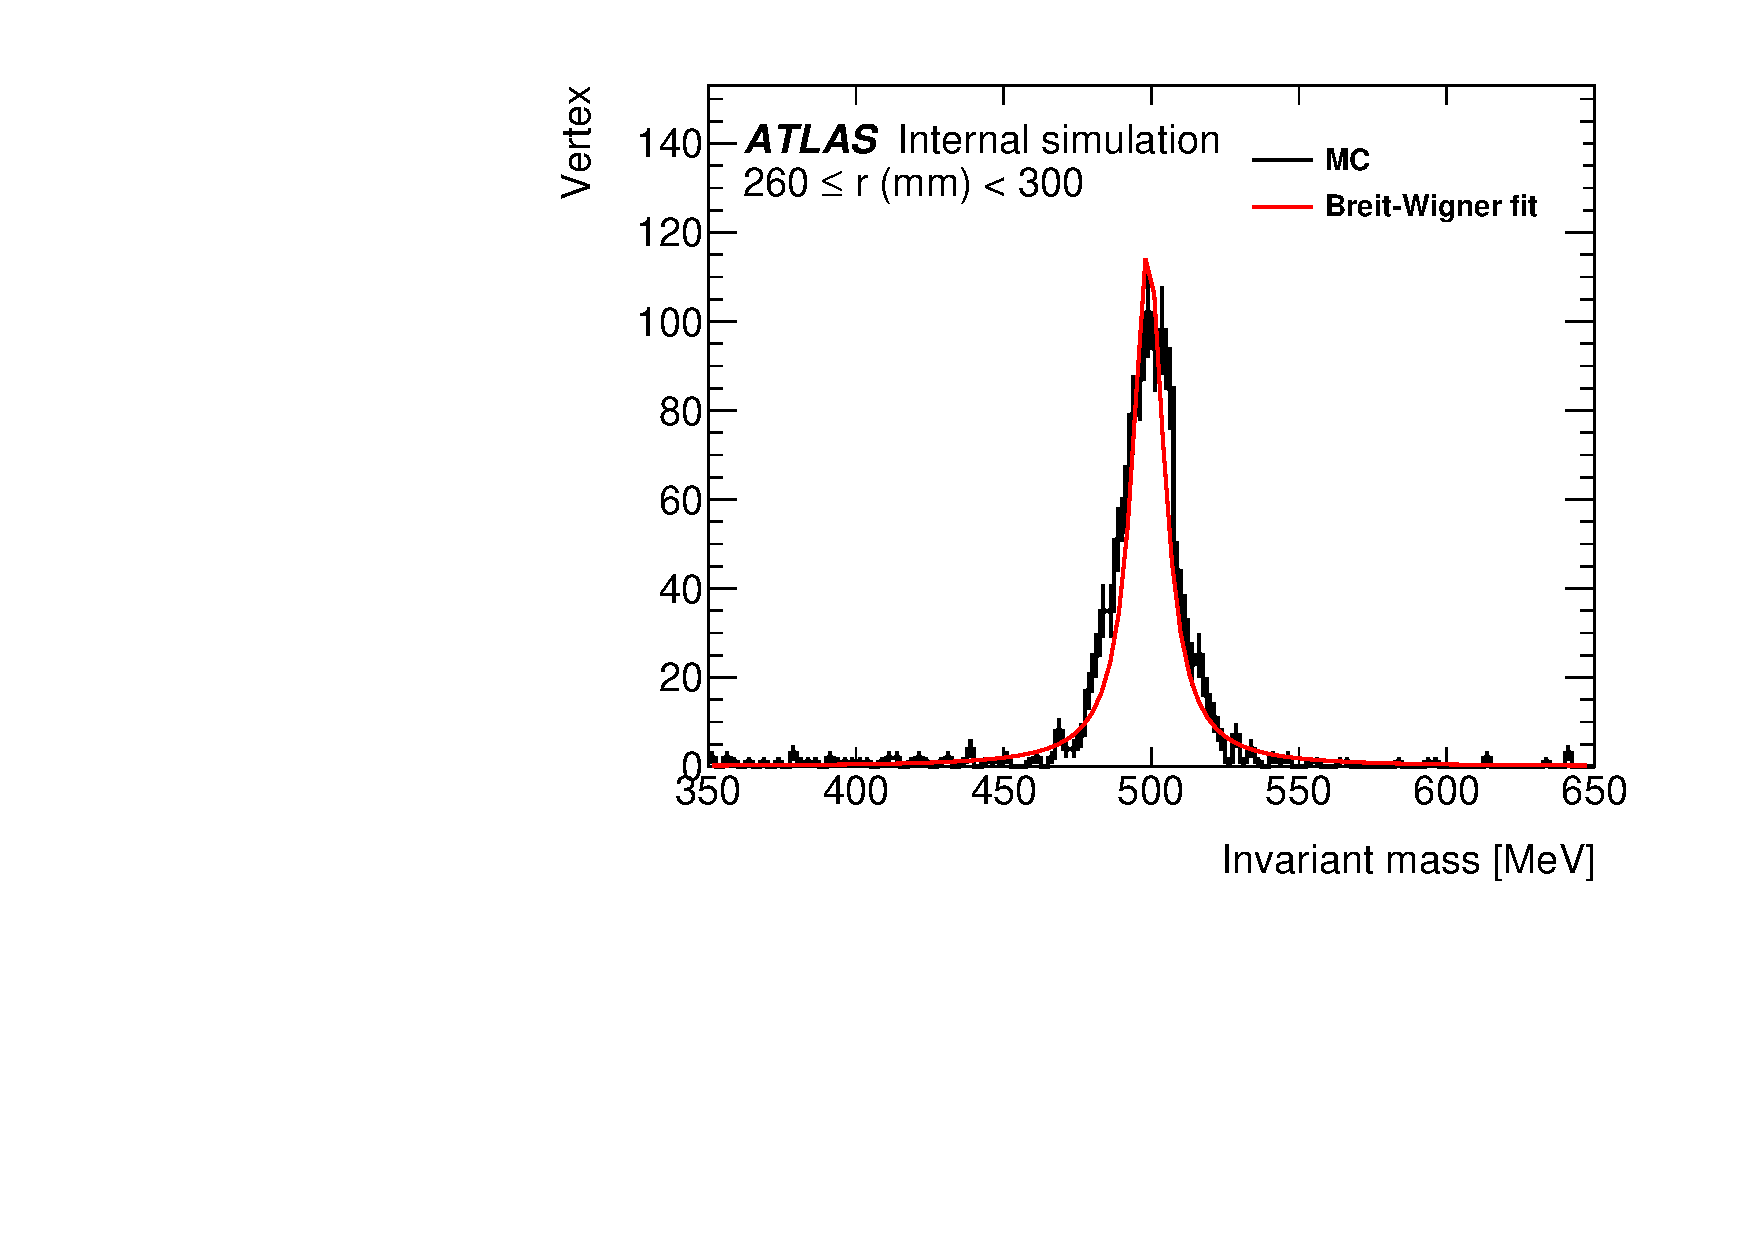
\includegraphics[width=0.33\textwidth]{figures/m_syst_Ks_Combined_MC_8}} \\
    \subfloat[Data, $r<20$ mm]{\label{subfig:Ks_fit_Data_1}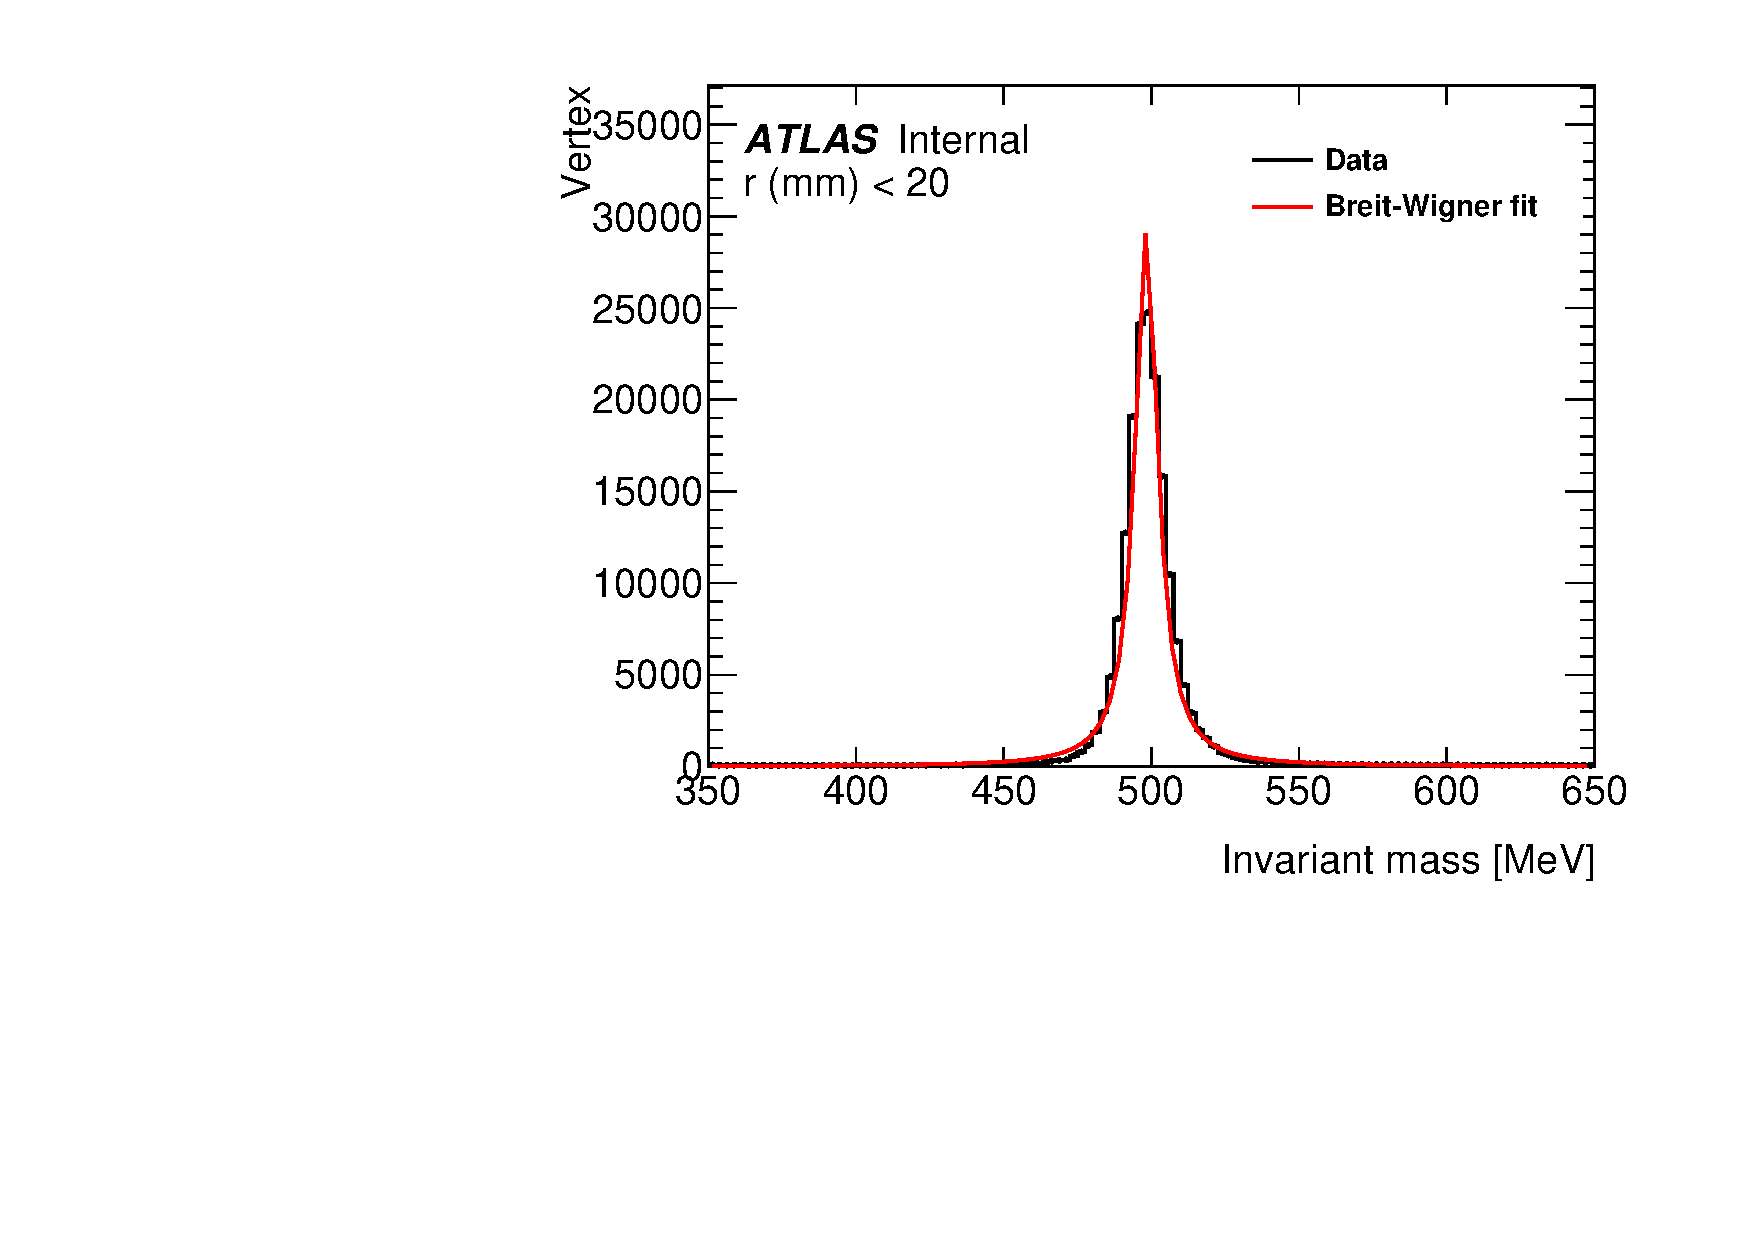
\includegraphics[width=0.33\textwidth]{figures/m_syst_Ks_Data_1}}
    \subfloat[Data, $100$ mm $<r<$ 140 mm]{\label{subfig:Ks_fit_Data_4}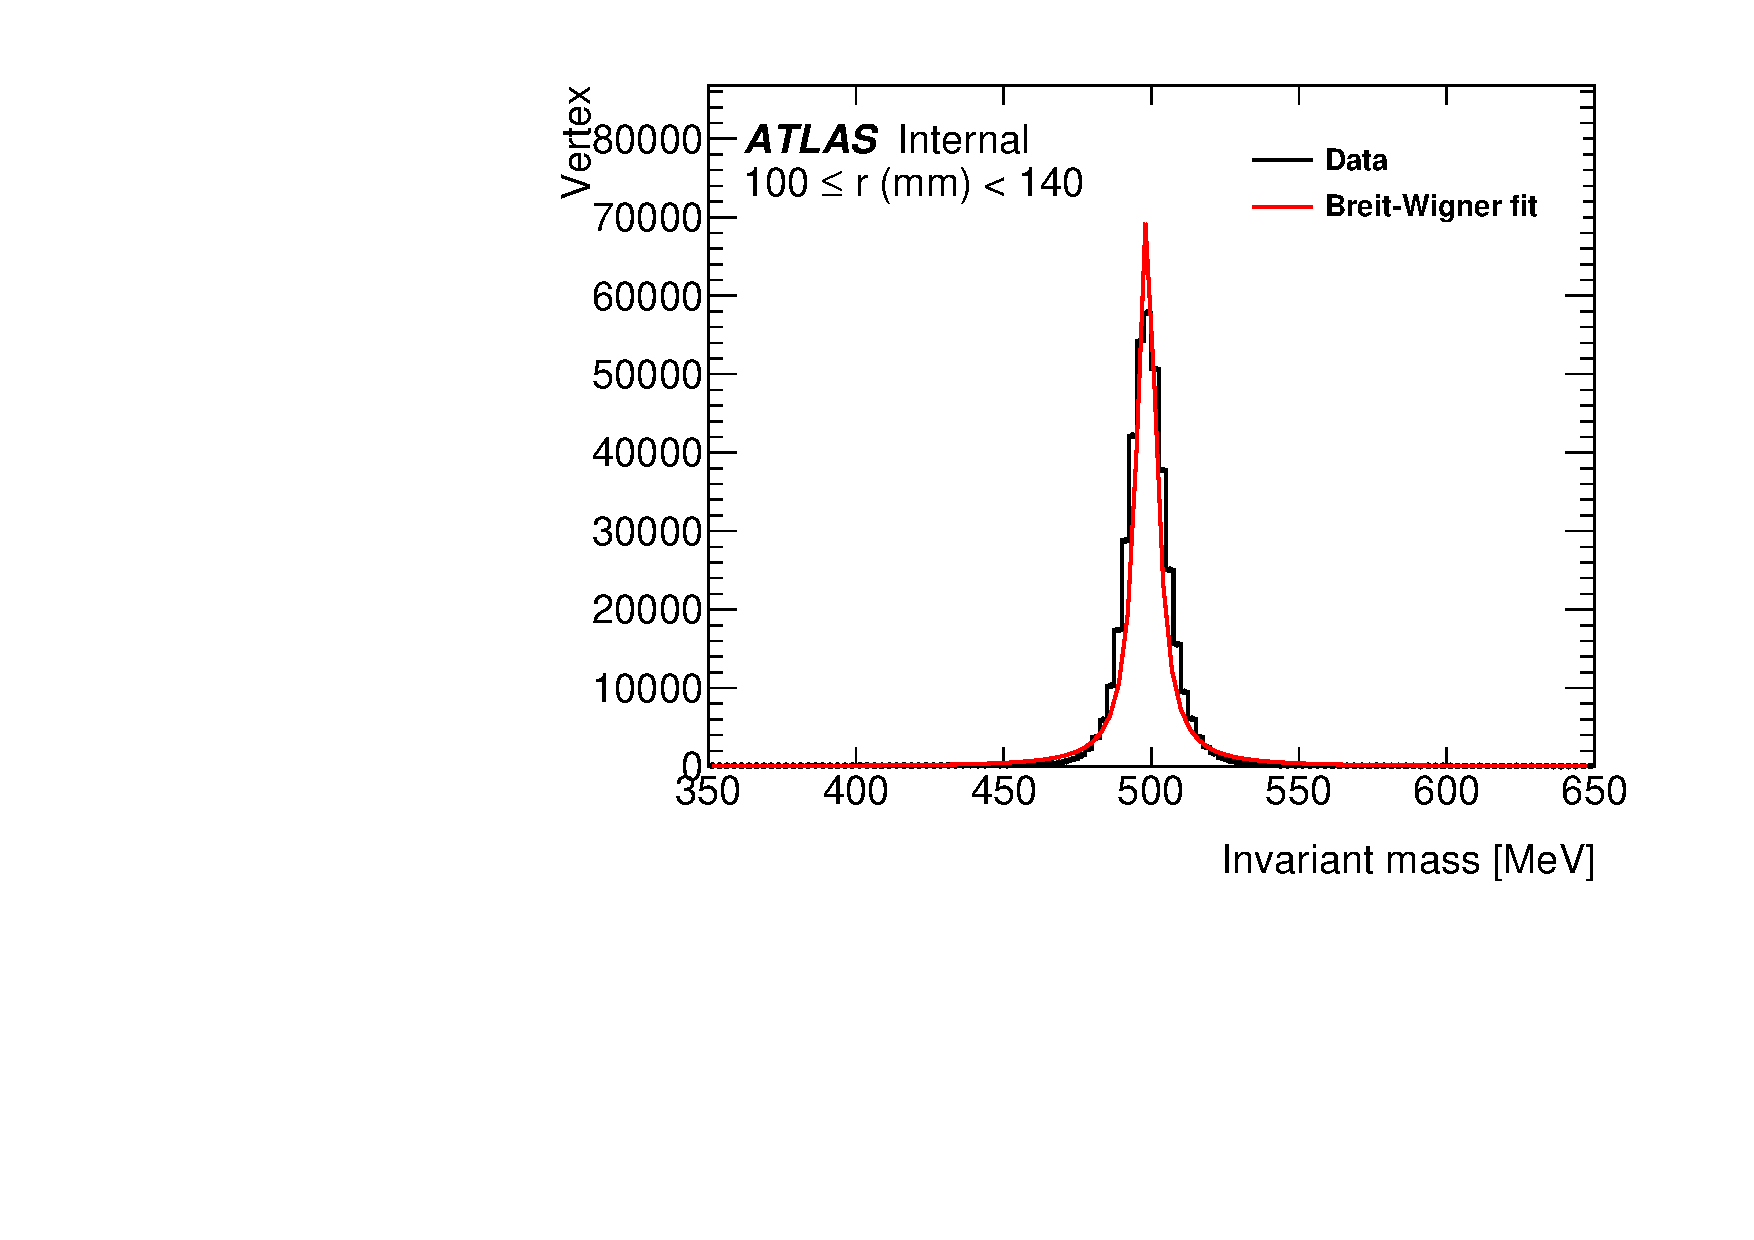
\includegraphics[width=0.33\textwidth]{figures/m_syst_Ks_Data_4}}
    \subfloat[Data, $140$ mm $<r<$ 180 mm]{\label{subfig:Ks_fit_Data_5}\includegraphics[width=0.33\textwidth]{figures/m_syst_Ks_Data_5}} \\
    \subfloat[Data, $180$ mm $<r<$ 220 mm]{\label{subfig:Ks_fit_Data_6}\includegraphics[width=0.33\textwidth]{figures/m_syst_Ks_Data_6}} 
    \subfloat[Data, $220$ mm $<r<$ 260 mm]{\label{subfig:Ks_fit_Data_7}\includegraphics[width=0.33\textwidth]{figures/m_syst_Ks_Data_7}}
    \subfloat[Data, $260$ mm $<r<$ 300 mm]{\label{subfig:Ks_fit_Data_8}\includegraphics[width=0.33\textwidth]{figures/m_syst_Ks_Data_8}} \\
    \caption{$K_{S}$ invariant mass for various $r$. The curve shows a fit to Breit-Wigner.}
    \label{fig:Ks_fit_all}
\end{figure}





\newpage

\section{$K_{S}$ and $Z'$ comparison}
\label{app:syst_Ks_Zp}
The ideal $K_{S}$ sample to estimate the systematic uncertainty in track and vertex reconstruction should have the same kinematic distributions as the $Z'$ MC sample. Obviously, the two samples have different distributions. Figure~\ref{fig:Ks_zp_comparison} shows comparisons of the vertex/kenematic distributions. The reconstructed $K_{S}$ and $Z'$ vertices are required to match to a $K_{S}$ and $Z'$ vertex produced at truth level with spatial displacement no larger than $0.7$ mm. All distributions are normalized to unity. It is fortuitous that their distribution cover the $r$ region of interest, and the two samples have similar $z$ distribution.


\begin{figure}[!htb]
    \centering
    \subfloat[]{\label{subfig:Ks_zp_r}\includegraphics[width=0.40\textwidth]{figures/m_syst_zp_Ks_r.pdf}}
    \subfloat[]{\label{subfig:Ks_zp_z}\includegraphics[width=0.40\textwidth]{figures/m_syst_zp_Ks_z.pdf}} \\
    \subfloat[]{\label{subfig:Ks_zp_eta}\includegraphics[width=0.40\textwidth]{figures/m_syst_zp_Ks_eta.pdf}} 
    \subfloat[]{\label{subfig:Ks_zp_pt}\includegraphics[width=0.40\textwidth]{figures/m_syst_zp_Ks_pt.pdf}} \\
    %\subfloat[]{\label{subfig:Ks_zp_z}\includegraphics[width=0.40\textwidth]{figures/m_syst_zp_Ks_DeltaR.pdf}}
    \caption{Distribution of transverse (a), longitudinal vertex position (b), $\eta$ (c), $p_{T}$ (d), and the opening angle between decay particles of $K_{S}$ and $Z'$ vertices (e) found in the background and the signal MC sample described in Section~\ref{sec:vertexing_systematics_Ks_zp_comparison}. Distributions are normalized to unity. Systematic uncertainties are shown.}
    \label{fig:Ks_zp_comparison}
\end{figure}



\newpage

\section{Track flipping extrapolation method}
\label{app:TF_extrapolation}
\subsection{Extrapolation from control region}
\begin{align}
\label{eq:TF_extrapolation_from_control}
N_{\mu x}^{est} &\approx 2 \cdot P(\mu) \cdot N_{xx}^{obs},\nonumber\\
N_{e x}^{est}   &\approx 2 \cdot P(e) \cdot N_{xx}^{obs}, \nonumber \\
N_{\mu\mu}^{est}&\approx P(\mu)^{2} \cdot N_{xx}^{obs}, \nonumber \\
N_{ee}^{est}    &\approx P(e)^{2} \cdot N_{xx}^{obs}, \nonumber \\
N_{e \mu}^{est} &\approx 2\cdot P(e)\cdot P(\mu) \cdot N_{xx}^{obs}.
\end{align}
where $N^{obs}$ and $N^{est}$ represent track-flipping vertex yield and estimated vertex yield by the extrapolation, respectively.

\subsection{Extrapolation from validation region}
\begin{align}
\label{eq:TF_extrapolation_from_validation}
N_{\mu\mu}^{est}&\approx \frac{1}{2} \cdot P(\mu) \cdot N_{\mu x}^{obs}, \nonumber \\
N_{ee}^{est}    &\approx \frac{1}{2} \cdot P(e) \cdot N_{e x}^{obs}, \nonumber \\
N_{e \mu}^{est} &\approx \frac{1}{2} \cdot (P(e) \cdot N_{\mu x}^{obs} + P(\mu) \cdot N_{ex}^{obs})
\end{align}

\subsection{Scale factors}
\begin{align}
\label{eq:TF_scale_factors}
S_{xx \rightarrow \mu\mu} &=  S_{xx \rightarrow \mu x}^{2}  \nonumber\\
S_{xx \rightarrow ee} &= S_{xx \rightarrow ex}^{2}  \nonumber\\
S_{xx \rightarrow e\mu} &= \Big(\frac{1}{2} (S_{xx \rightarrow \mu x} + S_{xx \rightarrow ex})\Big)^{2} \nonumber\\
S_{\mu x \rightarrow \mu\mu} &=  S_{xx \rightarrow \mu x}  \nonumber\\
S_{e x \rightarrow ee} &= S_{xx \rightarrow ex}  \nonumber\\
S_{e x, \mu x \rightarrow e\mu} &= \frac{1}{2} (S_{xx \rightarrow \mu x} + S_{xx \rightarrow ex})
\end{align}












%-------------------------------------------------------------------------------

%In an ATLAS note, use the appendices to include all the technical details of your work
%that are relevant for the ATLAS Collaboration only (e.g.\ dataset details, software release used).
%This information should be printed after the Bibliography.

\end{document}
